%%%%%%%%%%%%%%%%%%%%%%%%%%%%%%%%%%%%%%%%%
% Masters/Doctoral Thesis 
% LaTeX Template
% Version 2.5 (27/8/17)
%
% This template was downloaded from:
% http://www.LaTeXTemplates.com
%
% Version 2.x major modifications by:
% Vel (vel@latextemplates.com)
%
% This template is based on a template by:
% Steve Gunn (http://users.ecs.soton.ac.uk/srg/softwaretools/document/templates/)
% Sunil Patel (http://www.sunilpatel.co.uk/thesis-template/)
%
% Template license:
% CC BY-NC-SA 3.0 (http://creativecommons.org/licenses/by-nc-sa/3.0v/)
%
%%%%%%%%%%%%%%%%%%%%%%%%%%%%%%%%%%%%%%%%%


%----------------------------------------------------------------------------------------
%	PACKAGES AND OTHER DOCUMENT CONFIGURATIONS
%----------------------------------------------------------------------------------------

\documentclass[
%in original
11pt, % The default document font size, options: 10pt, 11pt, 12pt
%oneside, % Two side (alternating margins) for binding by default, uncomment to switch to one side
english, % ngerman for German
singlespacing, % Single line spacing, alternatives: onehalfspacing or doublespacing
%
%draft, % Uncomment to enable draft mode (no pictures, no links, overfull hboxes indicated)
%
%nolistspacing, % If the document is onehalfspacing or doublespacing, uncomment this to set spacing in lists to single
%
liststotoc, % Uncomment to add the list of figures/tables/etc to the table of contents
%toctotoc, % Uncomment to add the main table of contents to the table of contents
%parskip, % Uncomment to add space between paragraphs
%nohyperref, % Uncomment to not load the hyperref package
headsepline, % Uncomment to get a line under the header
%chapterinoneline, % Uncomment to place the chapter title next to the number on one line
%consistentlayout, % Uncomment to change the layout of the declaration, abstract and acknowledgements pages to match the default layout
]{MastersDoctoralThesis} % The class file specifying the document structure

% Required for inputting international characters
\usepackage[utf8]{inputenc}
% Output font encoding for international characters
\usepackage[T1]{fontenc}

% facilitate commenting
\usepackage{comment}

% Use the Palatino font by default
\usepackage{mathpazo}

% Use the bibtex backend with the authoryear citation style (which resembles APA)
%\usepackage[backend=bibtex,style=authoryear,natbib=true]{biblatex}

\usepackage[citestyle=authoryear,
			bibstyle=authoryear,
			natbib=true,
			backend=biber,
            maxbibnames=10,
			maxcitenames=2,
            giveninits=true,
            uniquename=init,
            terseinits = true,
            dashed=false
			]{biblatex}

% The filename of the bibliography
\addbibresource{bibliography.bib}

% Required to generate language-dependent quotes in the bibliography
\usepackage[autostyle=true]{csquotes}

% none of the packages worked as expected
\usepackage{textcomp} % to be able to use \textdegree

% package to handle units
\usepackage{siunitx}
% make a / to indicate "per"
\sisetup{per-mode=symbol}


% for prettier tables
\usepackage{booktabs} 

% use a glossary (file is still there if wanted)
%\usepackage[acronym,toc,nonumberlist]{glossaries} % use acronyms
%\makeglossaries

% to display code
\usepackage{listings}

% remove indentation
\setlength{\parindent}{0in}


%----------------------------------------------------------------------------------------
%	MARGIN SETTINGS
%----------------------------------------------------------------------------------------


% original page settings
% \geometry{
% 	paper=a4paper, % Change to letterpaper for US letter
% 	inner=2.5cm, % Inner margin
% 	outer=3.8cm, % Outer margin
% 	bindingoffset=.5cm, % Binding offset
% 	top=1.5cm, % Top margin
% 	bottom=1.5cm, % Bottom margin
% 	%showframe, % Uncomment to show how the type block is set on the page
% }

\geometry{paper= a4paper,
				left=5cm,%
                right=2cm,%
                top=2.25cm,%
                bottom=2.25cm,%
                headheight=12pt}%
   


%----------------------------------------------------------------------------------------
%	THESIS INFORMATION
%----------------------------------------------------------------------------------------

 % Your thesis title, this is used in the title and abstract, print it elsewhere with \ttitle
\thesistitle{Computer Vision Based Asparagus Classification}
%An analysis of gaze data quality of two simultaneously recorded eye trackers using a new extensive eye movement test battery}
\supervisor{Dr.\ Ulf Krumnack} % Your supervisor's name, this is used in the title page, print it elsewhere with \supname
\examiner{M.Sc.\ Axel Schaffland} % Your examiner's name, this is not currently used anywhere in the template, print it elsewhere with \examname
\degree{Master of Science} % Your degree name, this is used in the title page and abstract, print it elsewhere with \degreename
\author{Maren~Born, Michael~Gerstenberger, Katharina~Groß, Richard~Ruppel, Sophia~Schulze-Weddige, Malin~Spaniol, Josefine~Zerbe} % Your name, this is used in the title page and abstract, print it elsewhere with \authorname
\addresses{} % Your address, this is not currently used anywhere in the template, print it elsewhere with \addressname

\subject{Cognitive Science} % Your subject area, this is not currently used anywhere in the template, print it elsewhere with \subjectname
\keywords{Computer Vision, ANN, Supervised Learning, Semi-supervised Learning, Unsupervised Learning} % Keywords for your thesis, this is not currently used anywhere in the template, print it elsewhere with \keywordnames
\university{\href{https://www.uni-osnabrueck.de/en/home.html}{Osnabrück University}} % Your university's name and URL, this is used in the title page and abstract, print it elsewhere with \univname
\department{\href{https://www.ikw.uni-osnabrueck.de/en/home.html}{Institute of Cognitive Science}} % Your department's name and URL, this is used in the title page and abstract, print it elsewhere with \deptname
\group{\href{https://www.ikw.uni-osnabrueck.de/en/research_groups/computer_vision.html}{Research Group Computer Vision}} % Your research group's name and URL, this is used in the title page, print it elsewhere with \groupname
\faculty{\href{https://www.uni-osnabrueck.de/universitaet/fachbereiche/fachbereich_humanwissenschaften.html}{School of Human Sciences}} % Your faculty's name and URL, this is used in the title page and abstract, print it elsewhere with \facname


%%%%% BEGIN SECTION REDEFINITIONS
% Redefine different sections and section* to be of a higher level and
% introduce chapters, such that in the thesis the levels from the PeerJ journal
% can properly be reused.
\makeatletter

\let\oldChapter\chapter
\let\oldSection\section
\let\oldSubSection\subsection
\let\oldSubSubSection\subsubsection
\let\oldParagraph\paragraph

\def\section{\@ifstar\@section\@@section}
\def\@section#1{\oldChapter{#1}}
\def\@@section#1{\oldChapter{#1}}

\def\subsection{\@ifstar\@subsection\@@subsection}
\def\@subsection#1{\oldSection{#1}}
\def\@@subsection#1{\oldSection{#1}}

\def\subsubsection{\@ifstar\@subsubsection\@@subsubsection}
\def\@subsubsection#1{\oldSubSection{#1}}
\def\@@subsubsection#1{\oldSubSection{#1}}

\def\paragraph{\@ifstar\@paragraph\@@paragraph}
\def\@paragraph#1{\oldSubSubSection{#1}}
\def\@@paragraph#1{\oldSubSubSection{#1}}

\makeatother
%%%%% END SECTION REDEFINITIONS




\AtBeginDocument{
\hypersetup{pdftitle=\ttitle} % Set the PDF's title to your title
\hypersetup{pdfauthor=\authorname} % Set the PDF's author to your name
\hypersetup{pdfkeywords=\keywordnames} % Set the PDF's keywords to your keywords
}

\begin{document}

% Use roman page numbering style (i, ii, iii, iv...) for the pre-content pages
\frontmatter
\thispagestyle{empty}
%\pagenumbering{gobble}

\pagestyle{plain} % Default to the plain heading style until the thesis style is called for the body content


%----------------------------------------------------------------------------------------
%	TITLE PAGE
%----------------------------------------------------------------------------------------

\begin{titlepage}
	\begin{center}
		
		\vspace*{.06\textheight}
		{\scshape\LARGE \univname\par}\vspace{1.5cm} % University name
		\textsc{\Large Study Project}\\[0.5cm] % Thesis type
		
		\HRule \\[0.4cm] % Horizontal line
		{\huge \bfseries \ttitle\par}\vspace{0.4cm} % Thesis title
		\HRule \\[1.5cm] % Horizontal line
		 
		\begin{minipage}[t]{0.35\textwidth}
			\begin{flushleft} \large
				\emph{Authors:}\\
				\href{}{\authorname} % Author name - remove the \href bracket to remove the link
			\end{flushleft}
		\end{minipage}
		\begin{minipage}[t]{0.4\textwidth}
			\begin{flushright} \large
				\emph{Supervisors:} \\
				\href{https://www.ikw.uni-osnabrueck.de/en/research_groups/computer_vision/people/krumnack_ulf.html}{\supname} \\% Supervisor name - remove the \href bracket to remove the link 
                \href{https://www.ikw.uni-osnabrueck.de/en/research_groups/computer_vision/people/schaffland_axel.html}{\examname}
			\end{flushright}
		\end{minipage}\\[3cm]
		 
		\vfill
		
		\large \textit{The study report is submitted in partial fulfillment of the requirements\\ for the degree of \degreename}\\[0.3cm] % University requirement text
		\textit{in the}\\[0.4cm]
		\groupname\\\deptname\\[2cm] % Research group name and department name
		 
		\vfill
		
		{\large \today}\\[4cm] % Date
		%\includegraphics{Logo} % University/department logo - uncomment to place it
		 
		\vfill
	\end{center}
\end{titlepage}


%----------------------------------------------------------------------------------------
%	ABSTRACT PAGE
%----------------------------------------------------------------------------------------

\begin{abstract}
	% \addchaptertocentry{\abstractname} % Add the abstract to the table of contents
    % add content of Abstract tex file here
	Eye tracking experiments rely heavily on good data quality of eye trackers. 
Unfortunately, often only spatial accuracy and precision values are available from the manufacturers.
These two values alone are not sufficient to reasonably benchmark an eye tracker:
The values will deteriorate drastically during an experimental session due to head movements, changing illumination or calibration decay in general. In addition, different experimental paradigms allow to analyze different types of eye movements which cannot be evaluated by spatial accuracy or precision, for instance smooth pursuit movements, blinks or microsaccades.
To obtain a more comprehensive description of properties, we developed an extensive eye tracking test battery.
In 10 different tasks, we evaluated eye tracking related measures such as: the decay of accuracy, pupil dilation, smooth pursuit movement, microsaccade detection, blink detection, and the influence of head motion.
For some measures true theoretical values exist, for others, a relative comparison to a gold standard eye tracker is needed.
Therefore, we collected our gaze data simultaneously from a gold standard remote EyeLink~1000 (\SI{500}{\hertz}) eye tracker and the mobile Pupil Labs glasses (\SI{120}{\hertz} -- \SI{240}{\hertz}).
	
\end{abstract}


%----------------------------------------------------------------------------------------
%	ACKNOWLEDGEMENTS
%----------------------------------------------------------------------------------------

%\begin{acknowledgements}
%\end{acknowledgements}


%----------------------------------------------------------------------------------------
%	LIST OF CONTENTS/FIGURES/TABLES PAGES
%----------------------------------------------------------------------------------------

\tableofcontents % Prints the main table of contents

%----------------------------------------------------------------------------------------
%	THESIS CONTENT - CHAPTERS
%----------------------------------------------------------------------------------------

% Begin numeric (1,2,3...) page numbering
\mainmatter 
%\pagenumbering{arabic}

% Return the page headers back to the "thesis" style
\pagestyle{thesis}

% Include the chapters of the thesis as separate files from the Chapters folder

%----------------------------------------------------------------------------------------
%	INTRODUCTION
%----------------------------------------------------------------------------------------
\section{Introduction}

TODO: Introduction to the project and motivation behind it.

\subsection{The project}

TODO: Rough summary of the idea of the project.
How did the idea come up?
What is the project about?

\subsection{Background on computer vision based classification tasks}

TODO: Short introduction into the fields of machine learning, computer vision, and to artificial neural networks. Prospects and challenges of both on a general basis with respect to our issue. This part is kept brief.

\subsection{Background on sorting asparagus}

\begin{figure}[h]
	\centering
	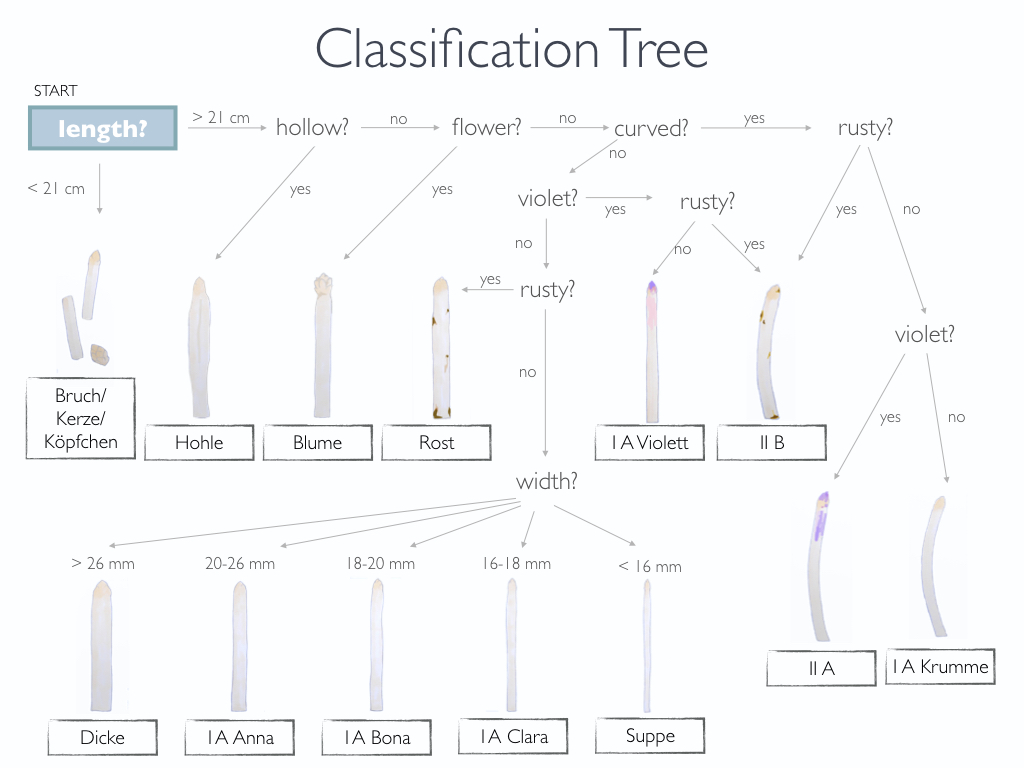
\includegraphics[scale=0.35]{Figures/chapter01/fig_tree_with_title}
	\decoRule
	\caption[Decision tree for labels]{The decision tree for attributing a label to the asparagus as to the sorting rules of the asparagus farm "Gut Holsterfeld". Starting from the upper left corner of the image binary decisions are made until a label is reached (except for Width).}
	\label{fig:LabelTree}
\end{figure}

TODO: What is the main focus during the sorting process, i.e. why do you need to sort asparagus and in which classes do you sort it? \\
What problems and challenges will be met - including the difference of challenge for humans vs. machines. \\
Including the description of the labels as sorted by Hof Gut Holsterfeld (Figure~\ref{fig:LabelTree}).


\subsection{Expected outcome vs. actual outcome of the project}

Based on the literature review, we aimed to improve the current sorting performance of the XX machine at the local asparagus farm “Spargelhof Gut Holsterfeld”. In this report, we investigated techniques from computer vision, both classical and deep learning based approaches. We expected to reach a result which is able to classify asparagus images into 13 different classes better than the current standard. For the initial performance of the sorting machine, no reliable accuracy of correctly sorted asparagus pieces is available, but between three and six workers are employed to re-sort wrongly classified asparagus pieces. The farmer himself assumes an accuracy of not more than 70\%. \\
 
An advantage of our project is that it was directly supported by the local asparagus farm, providing training data and allowing us to evaluate our proposed solutions in a real environment during the asparagus harvesting season 2020. \\
\\
However, there was a misunderstanding between us and the supporting asparagus farm about the kind of data we need. The existing images were too few, and also unlabelled. Therefore, we spent the first two and a half months with data acquisition instead of starting with preprocessing as we originally planned. Throughout the harvesting season 2019, we continuously went to the asparagus farm and collected unlabelled asparagus images during the normal harvesting procedure. For a small amount of asparagus pieces (xx in total), we collected labelled data by taking images of pre-sorted asparagus pieces. Pre-sorted in this context means that the asparagus pieces were sorted by the sorting machine and if needed re-sorted manually by professional workers. \\
The number of labelled images is insufficient to learn classes using deep learning approaches~\citep{russakovsky2013detecting} ~\citep{russakovsky2010attribute} (\url{https://petewarden.com/2017/12/14/how-many-images-do-you-need-to-train-a-neural-network/}). Therefore, we spent six months preprocessing and labelling the data manually. Preprocessing involved: organizing the large number of images, renaming the files, so that the three images of one asparagus piece can be accessed together, and performing automatic feature extractions (ref to preprocessing).To label the images by hand, we wrote a custom application (reference hand-label-assistant). The final labelled data set contains over 10.000 (genaue Zahl an stangen) labelled asparagus pieces. Next, we worked on numerous classical and deep learning approaches (ref to chap 4). We reached several very interesting results which will be discussed in Chapter 4. Although we developed an end-to-end prototype, we did not deploy it onto the sorting machine for the harvesting season 2020. Even though some of our results are highly promising, it is therefore difficult to compare it to the current performance of the machine. \\
 \\
Hier noch ein Absatz mit den Inhalten aus der Conclusion – sobald diese steht. 




%----------------------------------------------------------------------------------------
%	DATA ACQUISITION AND PREPARATIONS
%----------------------------------------------------------------------------------------

\section{Organization and data acquisition}
\label{ch:DataAcquisition}

In the second chapter of the report, the first stage of the study project is discussed, namely organizing, researching, and collecting the data.

The first section of the chapter~\ref{sec:Roadmap}~\nameref{sec:Roadmap} gives an overview of the time management of the study group. It is followed by the subchapter~\ref{sec:Organization}~\nameref{sec:Organization} in which communication and teamwork are assessed. In~\ref{sec:DataCollection} \nameref{sec:DataCollection}, the acquisition of the data from the sorting machine Autoselect ATS~II is described in more detail. The last section~\ref{sec:Literature}~\nameref{sec:Literature} presents the retrieved literature concerning the issue of agricultural product classification with machine learning based approaches.

\subsection{Roadmap of the project}
\label{sec:Roadmap}

At the beginning of the project, a roadmap was created to structure the year into different working stages as well as to have an overview of the tasks and problems that needed to be addressed.

\begin{figure}[h]
	\centering
	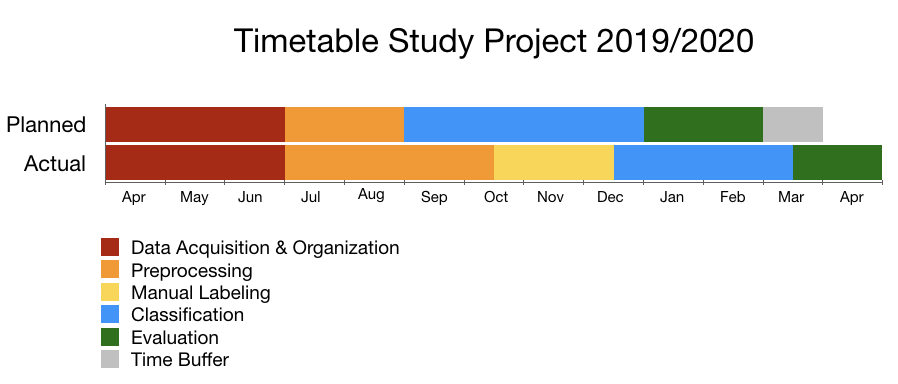
\includegraphics[scale=0.43]{Figures/chapter02/new_timetable.png}
	\decoRule
	\caption[Timetable of the Project]{\textbf{Timetable of the Project}~~~The upper timeline shows the estimated time of the study project from April 2019 to April/Mai 2020. The lower timeline displays how the time was spent. Both timelines differ in that the year was more optimistically planned than realized. A major factor was the lack of experience of the participants concerning the conduction of a larger project with many co-workers as well as concerning the general implementation of the preprocessing stage for machine learning classification. Another factor influencing the shifted timeline was the appearance of a fifth major stage, the \emph{Manual Labeling}.}
	\label{fig:Timetable}
\end{figure}

\begin{figure}[h]
	\centering
	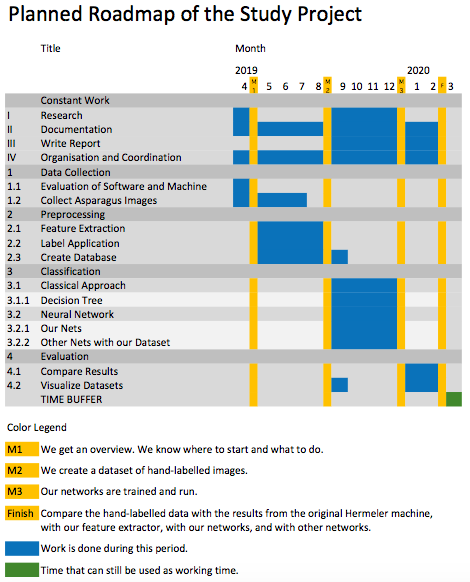
\includegraphics[scale=0.7]{Figures/chapter02/roadmap_planned.png}
	\decoRule
	\caption[Planned Roadmap]{\textbf{Planned Roadmap}~~~The figure shows the planned roadmap of the study project. It reveals how the time needed for each task was estimated in the beginning of the project.}
	\label{fig:RoadmapPlanned}
\end{figure}

\begin{figure}[h]
	\centering
	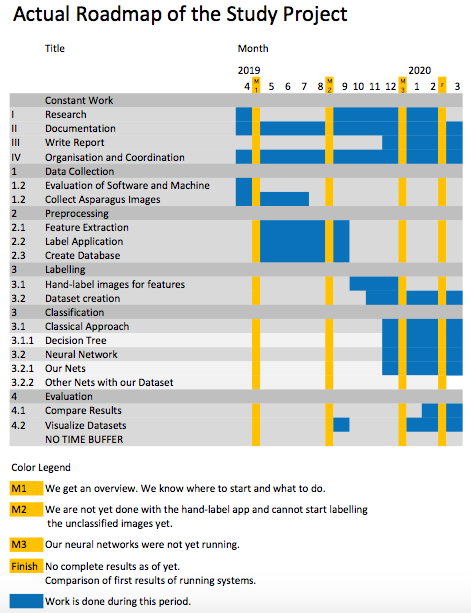
\includegraphics[scale=0.7]{Figures/chapter02/roadmap_actual.png}
	\decoRule
	\caption[Actual Roadmap]{\textbf{Actual Roadmap}~~~A roadmap that shows how the time was spent.}
	\label{fig:RoadmapActual}
\end{figure}

The timetable in~\autoref{fig:Timetable} gives a broad outline of the major stages of the project. In the upper timeline of the figure, it was estimated how much time for a specific phase is needed, whereas in the lower timeline the real time spent for the stage is given. Both timelines are structured to display the project year, starting in April 2019 and ending in April/Mai 2020. The months are represented by the x-axis while the colors mark the different working stages.

The project comprises four to five major stages: \textit{Data Collection \& Organization}, \textit{Preprocessing}, \textit{Manual Labeling}, \textit{Classification}, and \textit{Evaluation}. A detailed representation of the single tasks attributed to each stage can be found in the roadmaps in~\autoref{fig:RoadmapPlanned} and~\autoref{fig:RoadmapActual}. The project started with the data collection and the organization of the study project. During the first stage, the images were recorded with the sorting machine, while the major planning and research for the project took place. In the second phase, most of the preprocessing happened, that is, preparing and labeling the image data. The classification stage includes the time spent on the machine learning approaches which were implemented and trained on the asparagus data. In the last stage, the approaches were evaluated and their results were compared. The different stages overlapped to a certain degree. For the purpose of this figure, the start and end time is displayed as a hard boundary.

When comparing both timelines, some distinctions can be recognized. The upper timeline shows that preprocessing was estimated to be done by September. However, the phase continued until October, as can be observed in the lower timeline. Furthermore, the time for labeling a sufficient amount of images was underestimated, resulting in adjustments of the time attributed to this task. More specifically, it led to the \textit{Manual Labeling} of the image data receiving its own phase in the timetable, independent of the preprocessing phase.

The differences are depicted with different color codings. While the main focus of this project was supposed to be the application of different machine learning techniques to classify the data (color-coded in blue and green), the preprocessing phase and the data set creation/manual labeling posed to be most time-consuming (color-coded in orange and yellow).

In~\autoref{fig:RoadmapPlanned} and~\autoref{fig:RoadmapActual}, the stage specific tasks can be seen in more detail. Again, both figures display the estimated time and the actual time, respectively. The headlines serve as a division into the major stages except for the first heading, \emph{Constant Work}, which shows the tasks that demanded continuous attention and effort throughout the year. The duration of tasks is represented in blue, while the yellow lines mark milestones that are explained in the legends.

\subsection{Organisation of the study group}
\label{sec:Organization}

In this chapter, the management of the work distribution and the communication are taken into focus. For this the tools that were used for communication and organization will be examined as well as the structure of the group work.


\subsubsection{Communication}
\label{subsec:Communication}

The main communication consisted of weekly meetings in which the working process was discussed and new tasks were distributed. In addition to those meetings, different platforms were used, which worked with varying degrees of success. Used platforms were Asana, GitHub and Telegram to facilitate the communication aside from group meetings. The different means of communication will be described and evaluated in the following section.

\bigskip
Regular meetings made up the core organization of our project. During the meetings a discussion leader and a protocol writer were picked.\footnote{The protocols were saved for review in the GitHub project at \\ \url{https://github.com/CogSciUOS/asparagus}} The meetings were characterized by long discussions about how to approach the upcoming project step and how to tackle the next challenge. The project’s supervisors were usually present at the meetings, to bring in their expertise and to give the opportunity to ask concrete questions. During the first half of the project, tasks were distributed at the end of each meeting. In the subsequent meeting the working progress was discussed. This procedure was changed in the second half of the project. A schedule was used that described the different tasks and deadlines in detail. Additionally, we regularly gathered for co-working. The organizational meetings were continued, during which everyone gave precise and structured reports on their area of responsibility. This helped us to spend less time discussing and have more time for task-relevant work.

The majority of important information was exchanged via Telegram~\footnote{Telegram is a cloud-based instant messaging service for the use on smartphones, tablets and computers.}.  Starting from the first meeting, we had a constant conversation in a group chat on Telegram, in which we informed each other about the status of the project as well as support each other by answering questions. The group chat also created space for mutual motivation when needed.

Additionally, Asana was used in the beginning of the project. The communication platform is usually used to distribute tasks and to communicate about them. Many integrations of other applications, such as Slack, can help to achieve this. However, the tasks were easier to distribute in direct consultation at physical meetings and results could be easier demonstrated or discussed. If we had relied on communication with Slack or other agreed services or applications, it might have made more sense, but Asana alone has proven to be inefficient in our use case.

During the project, it was further learned how to work with GitHub~\footnote{GitHub is a web-based popular platform using the version control system Git that helps developers to store and manage their code, and track and control changes to their project.}. Git allowed us to work from anywhere, which facilitated the workflow.

Furthermore, we were able to automatically create documentations via Sphinx. This means that by adhering to the style conventions, the protocols, work schedules, manuals, and code comments were automatically included in our documentation.\footnote{see our documentation at~\url{https://asparagus.readthedocs.io/en/latest/}}


\subsubsection{Teamwork}
\label{subsec:Teamwork}

This section starts by introducing the team members and their previous experiences. It is followed by a description of the practical aspects of teamwork, the working structure, and the distribution of project-relevant tasks.

\bigskip
The project was an initiative of one of the students. A large part of the project members knew each other in private but had not yet worked together. Further students joined the project after its public announcement to complete the team. Thus, the group consisted of members with varying degrees of knowledge about each other. The team was initially made up by Josefine Zerbe, Katharina Groß, Malin Spaniol, Maren Born, Michael Gerstenberger, Richard Ruppel, Sophia Schulze-Weddige, Luana Vaduva, Thomas Klein, and Subir Das. None of the members had yet worked together as such on a project of this scope. During the course of the project, three members left the team for various reasons. Thomas left in July due to a change in his study program. Further, Luana and Subir left in October to pursue different study projects.

The members brought a wide variety of backgrounds into the team through different bachelor programs or different majors in the broader field of Cognitive Science. In the beginning of the project, the team members had little to no experience in the application of computer vision or neural networks. The motivation of most students was to pursue new and interesting tasks in these fields. Four students had a theoretical background in computer vision, six students had gained some experience with neural networks through the course ``\acrshortpl{ann} with TensorFlow’’, taught at the University of Osnabr{\"u}ck. Some had also taken machine learning classes during their study program. Git was previously only used by three students, but none of them were experts on its usage. Further, the team had neither experience with the Grid system of the \acrshort{ikw}, nor with running jobs on different machines. None of the members had prior knowledge about project management or task organization on a broader level.

\bigskip
In the beginning, the team lacked some structure and a clear distribution of individual roles. One reason for this could have been the harmonious atmosphere between team members. Further tasks such as the trips to the asparagus farm strengthened the team spirit and the social interactions. Thus, the task distribution was  very dynamically structured by making every decision democratically. Most tasks were performed in smaller teams of two to three people.  During meetings, possible next tasks were formulated but  without assigning them to specific members or working groups. This resulted in a lot of unassigned tasks and a discontinuous workflow. 

In August, the organization was restructured. On the one hand, a new structure for task distribution seemed more appropriate, instead of a democratic distribution. On the other hand, the strengths of the individual team members should be used more efficiently. Some team members had less programming experience than others. They had difficulties realizing certain tasks in an equal time period and with the same precision as others. Although they had good ideas in terms of concept, these were not implemented quickly enough to include them into the project. Nevertheless, it gave the opportunity to acquire new programming skills. To integrate more of the strengths that the single team members brought and to tackle the issue of time management, it was decided to write a work schedule that distributed the work more appropriately, gave an overview of the tasks that still had to be done and showed how much time was left to do them.

The supervision of the work was divided into manager roles, which means that the work was split into different main fields. Each member was responsible for managing their assigned area, distributing tasks and keeping an overview of the relevant work inside their working field. The manager could be consulted for questions, when in need of discussion, or for feedback. The meetings became more effective due to the new structure, and there was less discussion concerning task distribution. 

Further, common working hours on campus were introduced. The common working hours ensured that questions and decisions that arose could be discussed in person. This was especially helpful when different tasks overlapped and required communication and agreement.

\bigskip
In conclusion, the team structure and the distribution of work changed over the course of the project. The strengths of single members were used more efficiently and the supervision of working areas led to a more structured time management and task distribution. 


\subsection{Data collection}
\label{sec:DataCollection}

In this section the asparagus sorting machine at Gut Holsterfeld is described. Then the process of collecting labeled and unlabeled data is reported.

The machine Autoselect ATS~II (2003) is designed for sorting white and green asparagus (see~\autoref{fig:SortingMachine}) \citep{autoselectanleitung}. The asparagus is arranged on a conveyor belt that runs it through the recording section of the machine. Here, a camera takes three pictures per asparagus spear (see \autoref{fig:SortingMachineSketch} and \autoref{fig:ExampleImagesAnna}). Small wheels on the conveyor belt rotate the asparagus in the meantime so that it can be photographed from several positions. In the best case, on each image a different side of the asparagus is recorded. The conveyor belt transports the spear further and it is sorted into a tray depending on the chosen class label by the machine. The sorting is based on the parameters for width, length, shape, curvature, rust, and color. A total of 30 criteria for classifying an asparagus spear are used to describe these parameters. The calculation of the single features is based on a classical analytical approach. For example, the parameter for color detection is composed of eight sub-parameters. Each spear is reviewed at different areas (the head of the asparagus, the area below the head, and the stem) and judged for its hue in percentage. The values are compared and, according to a threshold, the spear is sorted into a color category (e.g.\, white or violet). For all parameters, there is a minimal threshold and a maximal threshold. As another example, the parameter for width detection calculates at three points at the asparagus (top, middle, and bottom part). From these three values, an average value is calculated that decides in which category the asparagus is sorted. If an asparagus exceeds the maximal threshold for parameter detection, it is not recognized and cannot be sorted accordingly. The same holds for values below the minimal threshold. Thus, all parameters have to have an upper and a lower threshold, including parameters that decide the presence of features like shape, curvature, and color. When evaluating what parameter boundaries to choose, it is recommended to check that most asparagus spears tend to be in between the average value and the maximal threshold, with a larger tendency to accumulate around the average value. Reportedly, the parameters and their respective ranges can be freely chosen by the user and can in this way be fitted to the needs of the respective asparagus farm~\citep{autoselectanleitung}.

\begin{figure}[!t]
	\centering
	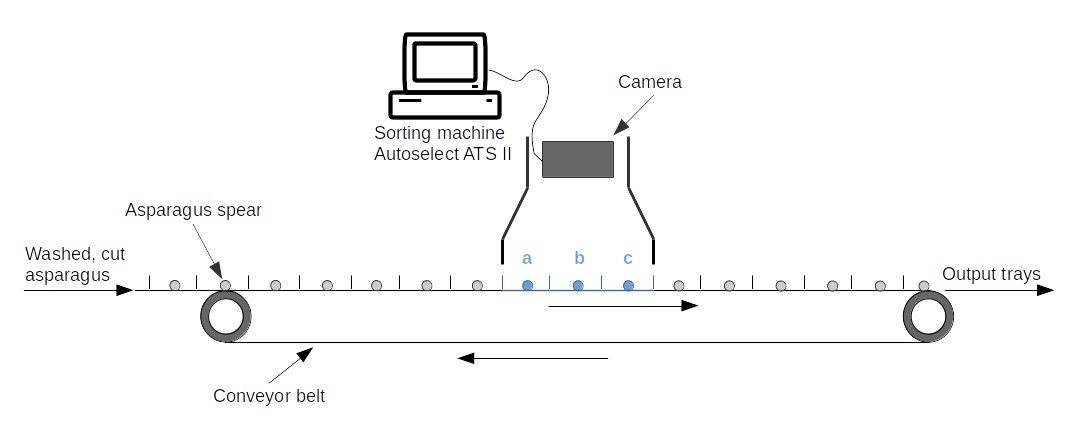
\includegraphics[width=0.9\textwidth]{Figures/chapter02/asparagusconveyerbelt_new.png}
	\decoRule
	\caption[Sketch of the Image Capturing Process with the Autoselect ATS II]{\textbf{Sketch of the Image Capturing Process with the Autoselect ATS II}~~~The asparagus spears are transported on a conveyor belt. After being washed and cut, the spears pass the camera field. Images are taken of three compartments, so that each asparagus spear is photographed three times in each position (a, b, c). The camera system is connected to a computer on which the sorting software runs. Depending on the resulting classification, the spear is sorted into the corresponding output tray.}
	\label{fig:SortingMachineSketch}
	\vspace{15pt}
	\centering
	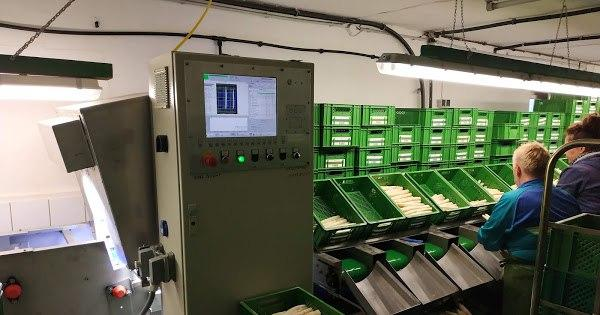
\includegraphics[scale=0.6]{Figures/chapter02/sortingmachine_front.png}
	\decoRule
	\caption[The Autoselect ATS II at Gut Holsterfeld]{\textbf{Autoselect ATS~II at Gut Holsterfeld}~~~In the figure the asparagus sorting machine Autoselect ATS~II at Gut Holsterfeld can be seen. The conveyor belt transports the asparagus from the left side of the image to the right side. It thereby passes the camera system. The display of the machine gives information on the parameters and the images. The machine is mainly controlled from here.}
	\label{fig:SortingMachine}
\end{figure}

\begin{figure}[!htb]
	\centering
	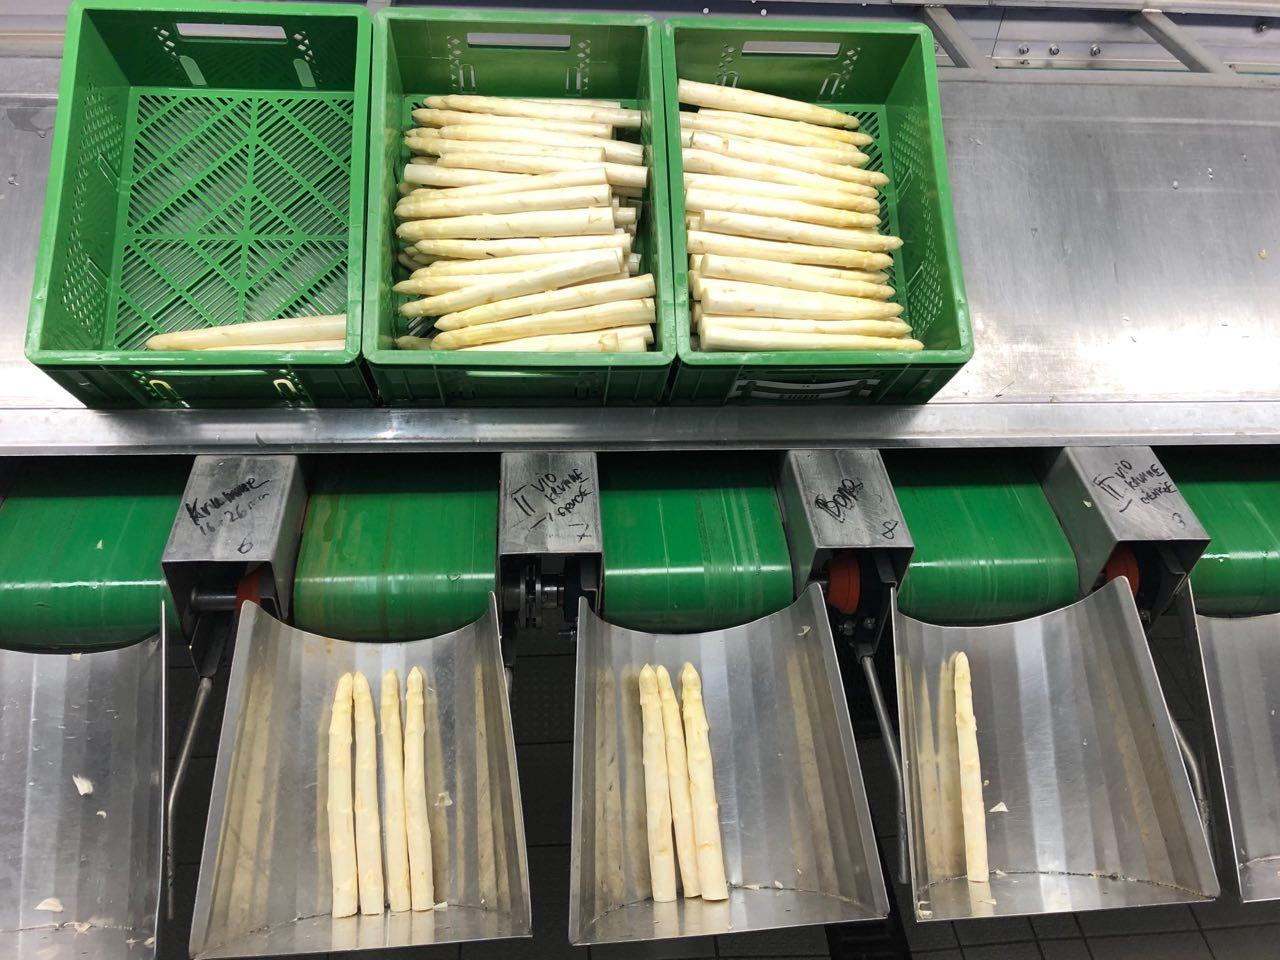
\includegraphics[scale=0.3]{Figures/chapter02/sorting_machine_slots.png}
	\decoRule
	\caption[Output Trays of the Sorting Machine]{\textbf{Output Trays of the Sorting Machine}~~~Depending on the class label, the asparagus is sorted into one of the machine's 16 trays.}
	\label{fig:SortingMachineSlots}
\end{figure}

Before the first use of the machine, all parameters are selected after a calibrating charge of asparagus has run through the machine. Then, the user can adjust the thresholds accordingly.

According to the manual, the number of quality classes is selectable. The user can define the order of quality classes by choosing the arrangement of parameters. The manufacturer suggests to first sort for length and width, then use the parameters that sort for color, and the parameters for shape detection last.

The accuracy of the sorting machine is described to be as good as 90\% best case by the manufacturer, while the farmer at Gut Holsterfeld reported it to be around 70\% at best, with re-sorting being necessary by professional sorters. Especially categories like Blume or Hohle were considered to be inconsistent by both, manufacturer and farmer. Further information could not be given on the software of the machine. A meeting with a representative of the engineering company HMF~\footnote{see \url{www.hmf-hermeler.de}}  that manufactured the sorting machine was arranged. Unfortunately, the source code itself was not available to HMF as it was produced by another company. 

\bigskip
In the following it is described how the image data was collected. It is possible to save images with the Autoselect ATS II, however, the storage space on the machine is very limited. Further, the selection of images to be saved is restricted to only 1000 images.
One workaround to the problem is the installation of the Teamviewer software~\footnote{see \url{https://www.teamviewer.com/en/}} on the machine and the connection of an external hard drive. After the installation, the process of image collection could be started remotely. This work was very ineffective and time-consuming. The data could not be directly transmitted to another computer because the internet speed at the farm is too slow. An automatic transfer of the images to the external hard drive was not possible until the installation of an automatic file moving service, for which the requirements are described below.

The file moving program needs to transfer the images to a new saving destination and has to run in the background without disturbing the workflow of the sorting machine. After research on background processes and programs, the decision was made to use a service, that is, a system process running independently of any program. The service manages moving the newly generated image files, as described in detail in the appendix in \autoref{subsec:FileService}.

The project members split in groups of two and exchanged the hard drive two times a week. The collected images were then transferred to storage capacities of the university.

The label that the machine attributes to each asparagus is not reliable. Therefore, sending the asparagus through the machine a second time would be the only way to gather labeled images. Unfortunately, a second sorting is not good for the quality of the asparagus. Further, at least one project member has to be involved in the re-sorting and, thus, has to be present at the farm. The sessions of exchanging the external hard drive and collecting labeled image data were combined.

\begin{figure}[!h]
	\centering
	\vspace{20pt}
	\begin{subfigure}{0.3\textwidth}
		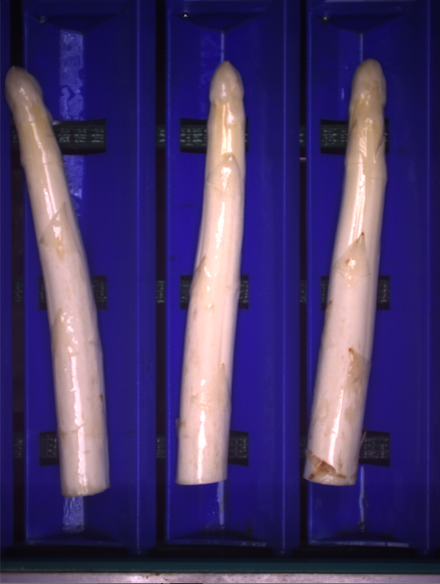
\includegraphics[width=0.95\linewidth]{Figures/chapter02/anna_a.png}
		\caption{left}
	\end{subfigure}
	\begin{subfigure}{0.3\textwidth}
		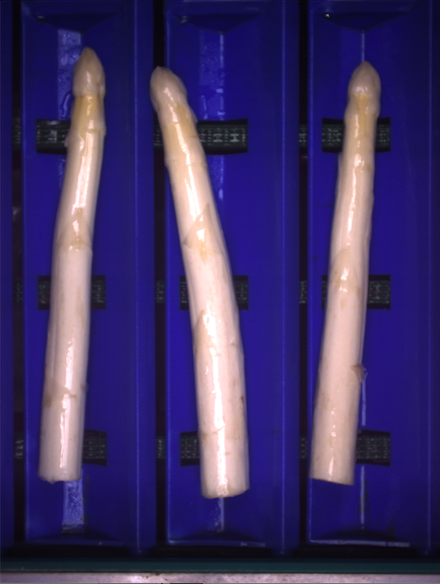
\includegraphics[width=0.95\linewidth]{Figures/chapter02/anna_b.png}
		\caption{middle}
	\end{subfigure}
	\begin{subfigure}{0.3\textwidth}
		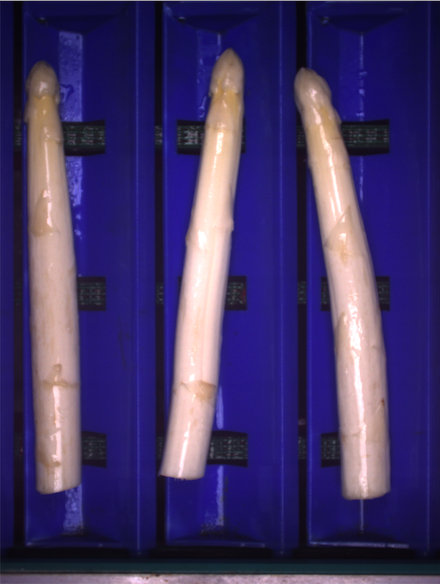
\includegraphics[width=0.95\linewidth]{Figures/chapter02/anna_c.png}
		\caption{right}
	\end{subfigure}
    \caption[Example Asparagus Images]{\textbf{Example Asparagus Images}~~~Example pictures of the quality class I~A~Anna. The asparagus is arranged on a conveyor belt that runs it through the recording section of the machine, where a camera takes three pictures. In picture (A) the target asparagus is to the left, in (B) it is in the middle, and in (C) it is to the right. Small wheels on the conveyor belt rotate the asparagus in the meantime so that it can be photographed from several positions. In the best case, on each image a different side of the asparagus is recorded. The conveyor belt transports the asparagus further and it is sorted into a tray depending on the chosen quality class by the machine. 
}
    \label{fig:ExampleImagesAnna}
\end{figure}

\bigskip
An example image of the received data can be seen in~\autoref{fig:ExampleImagesAnna}. There are three pictures per asparagus. The image resolution is $1040\times1376$ pixel per image, with an RGB color space.

\begin{table}[!htb]
	\centering
	\resizebox{.95\linewidth}{!}{%
	\begin{tabular}{|lr|lr|lr|}
		\hline
		\textbf{Class Label~~~~~} & \textbf{Nr. of Images} & \textbf{Class Label~~~~~} & \textbf{Nr. of Images} & \textbf{Class Label~~~~~} & \textbf{Nr. of Images} \\
		\hline
		I~A Anna		& 1005	& II~A	& 1051 	& Blume	& 1717	\\
		I~A Bona		& 908 	& II~B 	& 1468 	& Suppe	& 1157	\\
		I~A Clara	& 513 	& Rost 	& 1169	& Bruch	& 309	\\
		I~A Krumme	& 936 	& Dicke & 749 	& {}		& {}		\\
		I~A Violett	& 1514 	& Hohle	& 775 	& {}		& {}		\\
		\hline
	\end{tabular}%
	}
	\caption[Collected Images with Class Label]{\textbf{Collected Images with Class Label} \\ In this table, the number of collected images with a class label is reported. This was achieved by running pre-sorted spears a second time through the sorting machine}
	\label{tab:LabeledClassNumber}
\end{table}

In total, 612113 images were collected, with each class label being represented with at least 309 images, corresponding to 103 asparagus.

At the asparagus farm Gut Holsterfeld, 591495 labeled and unlabeled images were collected with the Autoselect ATS~II. The number of unlabeled data is 578226 images, thus, around 192742 different asparagus spears. Of the labeled data, the number of images that were collected per quality class can be found in \autoref{tab:LabeledClassNumber}. The image number does not represent the number of different asparagus spears, as each asparagus spear is represented by three distinct images.

\begin{figure}[!ht]
	\centering
	\vspace{20pt}
	\begin{subfigure}{0.3\textwidth}
		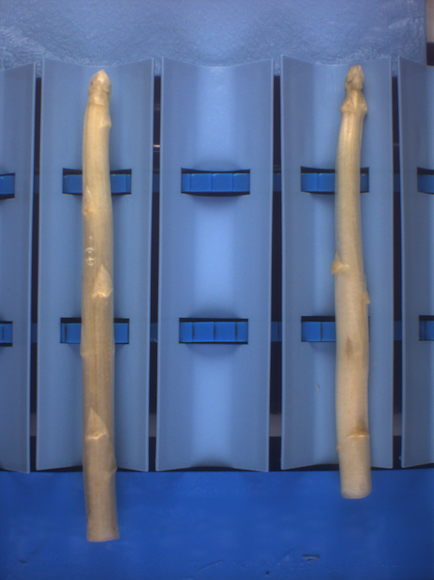
\includegraphics[width=0.9\linewidth]{Figures/chapter02/querdel_a.png}
		\caption{left}
	\end{subfigure}
	\begin{subfigure}{0.3\textwidth}
		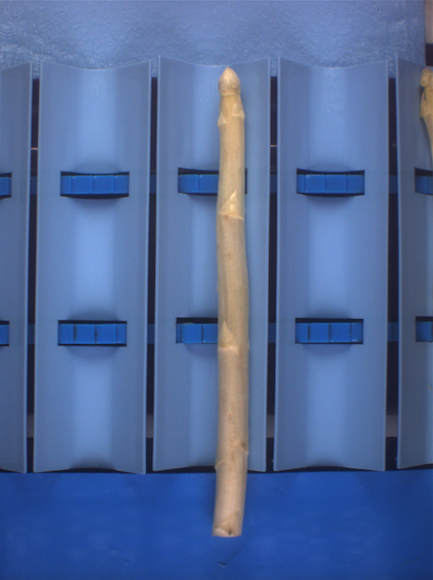
\includegraphics[width=0.9\linewidth]{Figures/chapter02/querdel_b.png}
		\caption{middle}
	\end{subfigure}
	\begin{subfigure}{0.3\textwidth}
		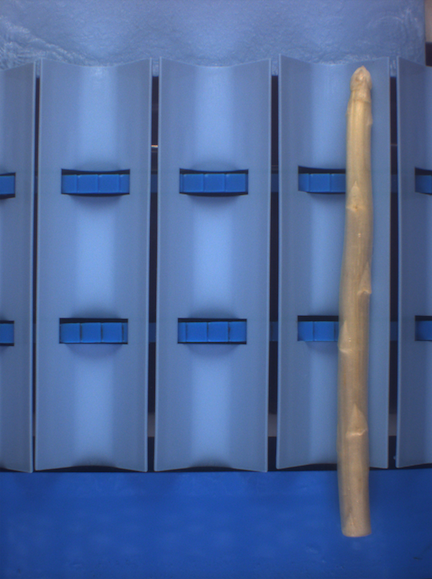
\includegraphics[width=0.9\linewidth]{Figures/chapter02/querdel_c.png}
		\caption{right}
	\end{subfigure}
	
	\begin{subfigure}{0.3\textwidth}
		\vspace{10pt}
		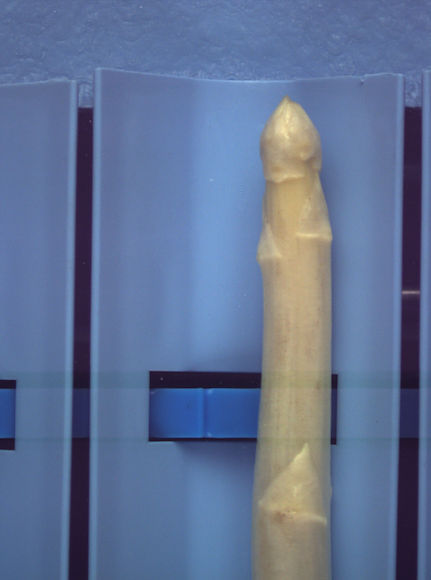
\includegraphics[width=0.9\linewidth]{Figures/chapter02/querdel_d.png}
		\caption{upper part}
	\end{subfigure}
    \caption[Example Asparagus Images Querdel's Hof]{\textbf{Example Images Querdel's Hof}~~~Example pictures of the asparagus of the farm Querdel's Hof. In picture (A), the asparagus spear is to the left, in (B), it is in the middle, and in (C) it is to the right. A fourth picture (D) is taken with a second camera with focus on the upper part of the asparagus.}
    \label{fig:ExampleImagesQuerdel}
\end{figure}

Additionally, a few images could be recorded at another asparagus farm, Querdel’s Hof~\footnote{see~\url{https://www.querdel.de/}}, in Emsb{\"u}ren. The farm sorts the asparagus with an updated version of the Autoselect ATS~II at Gut Holsterfeld, that is, it uses the same software but other hardware. In particular the resolution of the camera was improved and a second camera was installed that focuses on the head region of the asparagus. At Querdel’s Hof, 20616 images were collected in total, 76 from the class label ``normal’’, 152 from the class label ``violet/flower’’, and 20388 unlabeled images. Each asparagus spear is represented by four images: three images show the asparagus from different perspectives and a fourth image depicts solely the head region. Example images for one asparagus can be seen in~\autoref{fig:ExampleImagesQuerdel}. No internet connection could be established to the farm, thus, no further images were collected. Moreover, the data format of the images from Querdel’s Hof is different to the data from the farm Gut Holsterfeld, due to the additional head image. Therefore a combination of both data sets was not convenient. 


\subsection{Literature on food classification using computer vision}
\label{sec:Literature}

In the classification of food products, there are numerous possibilities to apply classical machine learning and \acrshort{ann} approaches for classification tasks on image data~\citep{bhargava2018fruits,brosnan2002inspection}.


For the scope of this investigation, we decided to focus our literature search on fruit and vegetable quality evaluation using computer vision and machine learning. Compared to other fields, research and evaluation in agricultural classification shares many characteristics and faces similar difficulties.

The quality inspection based on computer vision is usually constituted into five main steps: image acquisition, preprocessing, image segmentation, feature extraction and classification~\citep{bhargava2018fruits}. Moreover, most data in agriculture is based on photographic images. Also the features of interest are similar for different kinds of fruit or vegetable. Frequently by traditional computer vision techniques inspected features concern color, shape, size, texture, and defect~\citep{bhargava2018fruits}. This makes other papers in the field of agricultural evaluation directly comparable to our case. Moreover, we hope to get an impression of the state of the art of how many images are needed in our case, how high the image resolution needs to be, what kind of computer vision approaches could be helpful as a starting point,  and also to become aware of known challenges.

\bigskip
None of the found papers were suitable as blueprints for the asparagus classification project. However, some of them helped to get an idea of how to proceed with the project. For example, some papers show how the preprocessing phase could be structured~\citep{mery2013automated}, or they evaluate the machine learning methods that were already used on other food classification tasks~\citep{bhargava2018fruits}. Further, some of the literature is concerned with the classification of food products but not with differentiating between as many classes as 13~\citep{diaz2004comparison,kilicc2007classification}. Often, the variance in the food products, that is, the quality as well as the type of food used is either too high~\citep{zhang2012classification} or too low~\citep{kilicc2007classification,al2011dates} in comparison to the variance in our project data.  One paper evaluates the sorting of asparagus, however, it only does so on a small data set with three categories of green asparagus~\citep{donis2016classification}. Further papers on food classification are not detailed enough in their explanations and do not share the information needed for replication~\citep{pedreschi2016grading}. Another paper is mainly about the implementation of a certain toolbox~\citep{mery2013automated}.

Even though no specific paper was used as guidance to our project, some specific papers inspires us to try out certain algorithms, such as PCA ~\citep{Vijayarekha2008, Zhu2007}) or neural networks ~\citep{Jhuria2013, Pujari2014}. Moreover, the literature review made us aware of the limiting fact that images of fruits and vegetables are captured mainly from one direction~\citep{bhargava2018fruits}.The literature suggests that performance might improve, if more perspectives are taken into account. Moreover, the literature shows that different authors use different color spaces such as CIE Lab, RGB or HSI ~\citep{Liming2010, Garrido-Novell2012, Kondo2010}. This further inspired us to apply color quantization on our data.

\bigbreak
As the available data was only sparsely labeled, further research was done to evaluate the use of a semi-supervised learning approach~\citep{olivier2006semi,zhu05survey}. Details about the corresponding literature can be found in~\autoref{sec:SemiSupervisedLearning}. In regards to deep learning-based approaches, classical neural networks -- such as AlexNet \citep{alexnet2012original}, \acrshort{vgg}16/\acrshort{vgg}19 \citep{vgg2014original}, GoogleNet \citep{googlenet2015original}, Capsule Networks \citep{capsulenet2017original},  DenseNet \citep{densenet2017original}, ResNet \citep{resnet2016original} or \acrfull{nin} \citep{lin2013network} -- were assessed for better understanding of the range of possible pre-trained networks and ideas for network structures. Also, classical computer vision approaches were considered, like multiclass \acrfullpl{svm} \citep{prakash2012multi}.

%----------------------------------------------------------------------------------------
%	PREPROCESSING PIPELINE AND DATASET CREATION
%----------------------------------------------------------------------------------------
\section{The dataset}

Before implementing any approach that lets us predict a label to a respective asparagus, the recorded image data has to be preprocessed and arranged in a sensible format making it accessible (or even simpler to work with) for any computer algorithm. We are going to describe in detail how the raw images were processed into a dataset that is ready to use and how we obtained labels for the supervised learning approach. Further, we will report the sorting criteria that we decided on and the evaluation of our label agreement. Also, we are going to outline the classical computer vision approaches that we used to detect certain features from the image data without a machine learning process. \\
\\
As a first step, the images were loaded and saved on the IKW internal Grid, where the data was put in a fitting style and format. Then, the images had to be checked for any general errors that might have occurred during the recording and ordered in an understandable and structured way in the single folders on the Grid. \\
It was followed by different preprocessing steps where the three images of one spear were gathered at one location, and the removal of the background and any other unnecessary information in the images. Unfortunately, most of our collected data was not labelled and a solution to the issue of how to attribute a fitting label to each spear was needed. This proved to be no trivial task for the accumulated amount of data. \\
The first approach was to automatically extract the single features in the image which are responsible for a spear's label. The idea was to use classical machine learning approaches, f.e., a threshold for the RGB pixel values in the images, to obtain the individual features. As it was not possible to completely extract all the details from the pictures (especially features like the detection of a flower posed great difficulties) it was decided to label the images by hand. For that purpose, all implementable feature extraction functions were combined in an application (app). \\
The hand-label application has a graphical user interface where the user can click through the different feature categories, thereby indicating the presence of a feature. Some of the automatic feature extraction scripts were not able to classify an image on their own but could be used as an assistance to the user of the app. \\
The second approach was to manually label all images with the application, in that every member of the group had to look through a batch of asparagus images and note whether a certain feature from a set of previously defined features is present in the image.
The manual label process bore its own difficulties as vague images led to indecisiveness in the feature detection and a variance in the overall labelling agreement of the single members. The sorting agreement was therefore derived and used as a measurement of the overall goodness of the manual sorting process. \\
Finally, after all the different preprocessing and labelling steps were concluded, the dataset was built. To have a unified version of all labelled images and their respective labels, a reading function was created that enabled the later approaches presented in chapter 4 to assess the data. \\
\\
In this chapter, the different preparatory steps for the recorded data are described, including the creation of a dataset which is usable for any machine learning or computer vision approach to analyse the image data. \\
In 3.1 Preprocessing, the data was assessed and simplified for any further processing. \\
The second section, 3.2 Automatic feature extraction, is occupied with scripts researched and implemented for an automatic recognition of single features of the asparagus in the image. \\
The results were combined in an application which is described in more detail in 3.3 Manual labelling app. \\
In 3.4 Manual labelling, the process of hand-labelling the images with the application is described, followed by a section analyzing the results and comparing the overall agreement of the labellers. \\
The last section, 3.5 The asparagus dataset, concludes with the creation of the final dataset, used for the later training of the neuronal networks and other approaches to detect the label of a spear from its three images.



\subsection{Preprocessing}

An important, often underestimated, step of any machine learning project is the preprocessing. After collecting the data, it is mostly not in the right format yet, but needs to be altered for the particular purpose. \\
\\
In our case, the first step of the preprocessing was to combine the three perspectives of each asparagus piece. The sorting machine, that we are working with, takes images that show three compartments at a time and takes an image each time a new asparagus piece is in the center. That means, each asparagus can be found in three pictures, one in each of three positions - left, center and right. The names of the images can be used to combine the three relevant images and determine in which position the asparagus was captured. This way the images can be cut into three pieces and renamed in a way that makes it clear which images belong together. Each asparagus gets a unique identification number and the three perspectives are denoted with "a" for left, "b" for middle and "c" for right. For example, the image 42\textunderscore b.png is the middle image of the asparagus with the identification number 42. \\
The second step was to remove the background to get rid of as much of the unnecessary information as possible. As the conveyor belt that transports the asparagus pieces is blue in color and there is a high contrast to the bright asparagus pieces it could easily be removed. First the asparagus piece is masked using the color hue of the HSV representation of each image. Second, very dark regions are added to the background based on a mask retrieved by thresholding the value component. This is particularly important for the automatic feature extraction as one can see in the following chapter. Additionally, the asparagus was rotated upwards for some of the applications to reduce the variance that is due to differences in the angle, in the hope of making the machine learning task (that has to be accomplished by the classifiers) more simple and hence reducing the required number of samples. This is especially important as labels had to be generated manually. Moreover, reducing variance in dimensions that are irrelevant with respect to the properties of interest is a prerequisite to apply unsupervised methods such as PCA or autoencoders and the semi-supervised approaches that are based upon the earlier as. This is achieved by binarizing into foreground and background pixels, calculating the centerline as the mean pixel location along the vertical axis and fitting linear regression to the centerline pixels. The estimate for the angle are retrieved using arcus tangens 2 and the depictions are rotated accordingly. Thereby, another dataset was created. \\
\\
During preprocessing the raw images are collected, sorted by name and the three perspectives of each piece are identified. Then, the images are cut into three parts and the left, middle or right part is kept, respectively. Afterwards, the background is removed, which means pixels that are not part of the asparagus are set to zero.  This is done by masking all pixels with a blue hue in HSV color space and all pixels that are not bright enough as background and set them to zero. On top of that, all connected regions that remain after removing background pixels by hue and brightness are also removed except for the largest one. By doing that, any distortions like reflections or single noisy pixels are set to zero and only the asparagus piece itself remains. The only faulty areas that can be left over with this approach are areas that are connected to the asparagus. But as this is only rarely the case, its effect is neglectable. The position of the asparagus within each cutted image was further improved by centering the fragments of the image around the center of mass. This way the asparagus is always in the middle. If the new cutting line falls out of the image boundaries, the missing area is filled with zeros, too. \\
\\
It should be noted that, although it is an advantage to have several perspectives on the asparagus, as some features might only be visible from a certain side, it also bears some problems. Namely, the lighting and reflection are slightly different, which can alter the color values, and the images can be a little distorted. Hence, the asparagus might appear wider or smaller depending on the perspective. This makes it harder for classical computer vision algorithms to determine some features accurately. \\
\\
Another version of the dataset was computed by converting the depictions to color palette images. An appropriate palette and the respective mapping of RGB values to palette colors was determined using clustering in color space. First a set of RGB tuples is collected by adding pixel values for the depiction of 10.000 asparagus pieces. Second the resulting list of RGB tuples is converted to an image and third a palette is determined using an algorithm that determines the position of cluster centers while maximizing the  maximal coverage. The resulting cluster centers can be displayed as a list of RGB values and represent the color pallette~\citep{zarandi2011large} (\url{https://github.com/python-pillow/Pillow/blob/55e5b7de6c41b0386660b0bee7784ac04f412f4b/src/libImaging/Quant.c}). Each image of the downscaled version of the dataset was transformed to the palette representation. Visual inspection showed little quality loss such that it can be assumed that the relevant information for image classification is well preserved. \\ 
\\
Several additional datasets were computed based on the background removed version. This holds for downscaled versions as well as for a version that contains the asparagus heads only. To compute the latter the images were padded to avoid sampling outside of the valid image boundaries and the uppermost foreground row was detected. Subsequently the center pixel was determined and a snippet of the image was cropped such that this uppermost central pixel of the asparagus is contained as the center of the uppermost row of the snippet. The resulting snippets of asparagus heads are rotated using the centerline regression approach described above. The approach has proven reliable and the resulting depictions were used to train a dedicated network for head related features (see XXX).


\subsection{Automatic feature extraction}

Beside the main aim of this study project, to use machine learning algorithms to classify asparagus automatically, also classical computer vision methods were implemented for comparison. We used these methods to write algorithms that take the images as an input and return a prediction for the different features as an output. The goal was to predict the features reliable enough to deduce the corresponding class from them. \\
\\
According to the producer of this and other sorting machines, the softwares currently on the market use very similar methods, which gives us reason to believe that the classical methods might not be adequate to yield a better classification than the current status quo. Nonetheless, it is interesting to see, which features are harder to detect and which are easier. \\
The results vary greatly between the different feature extraction methods. While the functions to detect the width and length and whether the asparagus is violet or bended were good enough to be integrated into the hand label app to help us label, other features turned out to be more difficult. \\
\\
In the following, the different automatic feature extraction methods will be described, alongside with the results that were achieved and future steps that could be taken to improve the results further. For each feature detection method, the images with removed background were used.


\subsubsection{Length}

The length detection uses a pixel-based approach, it counts the number of rows from the highest to the lowest pixel that is not a background pixel and therefore not zero. The asparagus was rotated upwards, as described in chapter XX, in order to improve the results, as the rows between the highest and the lowest pixel are counted and not the pixels themselves. This technique is a simplification, which does not represent curved asparagus very well, because it will have a shorter count than it would have if the pixels were counted along the asparagus piece. But in reality, there are not a lot of asparagus pieces close to the decision boundary between broken and a whole piece. Usually, the asparagus is picked a few centimeters longer than necessary and then cut to the desired length. The only asparagus shorter than that length are the ones that break while in the sorting machine. And if they break they generally break closer to the center of the asparagus rather than at the ends of it. Therefore, the difference in length detection does not matter for our classification. \\
\\
All in all, the length detection yields good results that are very helpful for the label app. The next step would be to train a decision boundary that determines which number of pixels should be the threshold to differentiate between broken and not broken. At first, we tried to calculate this threshold by finding a conversion factor from pixel to millimeter, as we know the cut off in millimeters. But this approach appeared to be more difficult than anticipated, because the conversion factor varies in the different image positions. This problem only became apparent after the asparagus season had ended, for which reason we could not reproduce the camera calibrations in retrospective in order to take well-measured images, for example from a chessboard pattern. Accordingly, the threshold needs to be deduced from the data or learned with a machine learning approach.

\subsubsection{Width}

The width detection uses a very similar approach as the length detection as it takes the pixel count from the left-most to the right-most  pixel in a certain row as a width measure. But in contrast to the length, the width was measured at several different rows from which the mean width was taken. For the label app we decided that three measurements are sufficient, because asparagus spears usually do not show drastic changes in width at several positions. Hence, if there are larger changes at all, three evenly distributed positions should capture those changes well. \\
\\
The algorithm operates as follows: Firstly, the images are binarized into foreground and background, which means setting all pixels that are not zero, and therefore not background, to one. After that, the upper-most foreground pixel is detected and the length is calculated with the length detection function as described above. The length of the asparagus is used to divide it into even parts. This is done by determining a start pixel and dividing the remaining rows that contain foreground pixels by the number of positions one wants to measure at. This way several rows are selected in which the number of foreground pixels is counted. One can interpret each row as a cross-section of the asparagus, therefore the number of foreground pixels is a direct measure for the width. Then, the mean of these counts is calculated and used as the final width value. As the head of the asparagus can be of varying form and does not represent the width of the whole asparagus well, it is excluded from the measure. This is done by selecting a start pixel below the head area instead of naively choosing the uppermost pixel. To be precise, the start pixel is chosen 200 pixels below the uppermost pixel in order to bypass the head area with certainty. As described in the length detection, also in the case of the width detection curved asparagus pieces might lead to slightly different outcomes than the true values, but again this difference is regarded as irrelevant in our case.

\subsubsection{Rust}

The rust detection finds all pixels that fall in the range of RGB values that correspond to the color brown. Those pixels are counted and normalized by the maximal number of possible pixels that could be rusty, namely the number of foreground pixels. But as it is impossible that the whole asparagus is rusty and hence that all the foreground pixels fall into the relevant range of RGB values, this normalization yields small numbers as results. To give an example, an output value of 0.13 is already considered moderately rusty. The lower and upper bound for the RGB values are set to [50,42,30] and [220,220,55], respectively. That means, all pixels that have a red value between 50 and 220, a green value between 42 and 220 and blue value between 30 and 55 are considered as rust. \\
\\
Visual inspection shows that the rust detection algorithm works well to detect rusty areas and barely misses any rusty parts. But it is difficult to set a threshold for the number of pixels needed to be classified as rusty, because many pixels with a brown color that are distributed over the whole piece are not supposed to be classified as rust. Only clusters of brown pixels are a reliable indicator for rust. To make this intuition more clear, it could be the case that two asparagus have the same number of brown pixels, but in one case they are all connected building a cluster and in the other case they are evenly distributed over the whole asparagus piece. That would mean that, although both yield the same output value, only one of them should be considered as rusty. However, it should be mentioned that this is merely an artificial example to display one draw-back of the implementation. In reality, it is  very unlikely that an asparagus has a large number of brown pixels that are not in fact rust. \\
\\
Nevertheless, it remains unsolved to set a robust threshold that works well on the whole dataset. One problem that cannot be solved algorithmically, is dirt in the sorting machine. If the machine is not cleaned thoroughly and regularly, dirt can be falsely classified as rust as it often falls in the same color range. Another problem can be a change of lighting when taking the images. Both issues can be controlled for easily, but have to be communicated well to the farmers.

\subsubsection{Violet}

Especially when exposed to light asparagus pieces tend to change in color. An initial shift from the desired white appearance to a slightly rose or violet tone can be observed first. This change in colour, that is considered a flaw according to German quality standards, typically affects the head of asparagus pieces. However in some cases a non-uniform distribution of more or less violet areas can be observed. Moreover, it has been shown in practice that colour impression is highly subjective which manifested in discussions of edge cases during labeling. Effects of meta contrast potentially even affect the colour impression on an individual level. The lack of a formal definition for violet asparagus pieces also poses challenges to approaches of measuring this feature. \\
\\
In a simple approach to measure whether an asparagus piece is violet or not, colour hues are evaluated. More precisely, this strategy is based on evaluating histograms of colour hues that are calculated for foreground pixels of the asparagus images after converting them to the HSV colour space. Pale pixels are removed from the selection by thresholding based on the value component of the HSV representation. Finding the optimal threshold was proven difficult and corresponds to the abovementioned question of what it means for an asparagus spear to be violet. A value of 0.3 was considered a good compromise. All three perspectives were taken into account to compute one histogram per asparagus piece. A score was calculated by summing up the number of pixels that lie within a violet colour range. A second threshold was used as the decision boundary for violet detection. The direct and intuitive feedback in the label app showed the relation between varying thresholds and the prediction. It has shown that lowering thresholds also means the feature extractor becomes more sensitive at the price of a reduced specificity. Best overall matches (accuracies) with the subjective perception were found for very low thresholds. In many cases, however, measurements based on this definition of “violet” did not match the attributed labels. \\
\\
Hence, another sparse descriptor was derived from the input images. However, instead of thresholding pale values and calculating the histograms of colour hues this approach relies directly on the colours that are present in the depiction of an asparagus piece. As the 24 bit representations contain a vast amount of colour information in relation to the number of pixels it is, however, unfeasible to use these as an input. Instead the colour palette images can be used. Histograms of pallete images can serve as the basis to define the feature “violet” in a way that captures more of the initial colour information while being simple and understandable enough to allow for customizations by users of sorting algorithms or machines. As a consensus regarding such a definition is arguably hard to achieve and somewhat arbitrary the descriptor was used to learn implicit definitions of the feature (see XX). \\
\\
It has been shown that explicit ways of directly measuring, in how far an asparagus piece is violet can be implemented but heavily depend on the definition of this feature. As colour perception is highly subjective across and even within subjects machine learning approaches that are trained on human labelled data appear to be promising. Using them can help generalizing a definition for the degree to which an asparagus piece is violet.

\subsubsection{Curvature}

Multiple curvature scores can easily be computed based on regression fits to the centerline of an asparagus piece. For example, the parameters of linear or polynomial regression can be interpreted as a description of the curvature of an asparagus spear. However, the question remains if a scalar descriptor that matches with the subjective definition can be derived. \\
\\
Deriving sparse descriptions is based on a two stage approach. In the first stage, the centerline of an asparagus piece is computed because it is considered to be a good description of the curvature of asparagus pieces. Preprocessed images are used as the input where the background is removed and replaced by black pixels. Each asparagus piece is approximately oriented vertically. The centerline is computed by binarizing the image into foreground and background and computing the mean of pixel locations along the vertical axis (i.e. for each row). The resulting binary representation shows a single pixel line. It serves as the input to the second stage of curvature estimation.
In the second stage, curves are fit to the pixel locations of the centerline. For the simplemost score, linear regression is employed and the sum of squared errors is thresholded and interpreted as a curvature score. This score is small for perfectly straight asparagus pieces and increasingly large for bent ones. As an S-shaped piece is arguably perceived as bent even when the overall deviations from the center line are small a second descriptor was computed as the ratio between the error of a linear fit and polynomial regression of degree three. Thresholding values and employing a voting scheme (e.g. at least one value indicates curvature) for the results for all three perspectives yields a rule to measure curvature. However, it has again proven difficult to set thresholds appropriately to reliably capture the visual impression. Hence, another sparse representation was calculated by fitting linear regression to each of six segments of each depiction of an asparagus piece. An MLP was trained on the resulting 18 angles per piece (see XX). \\
\\
Calculating a score for curvature is fast and efficient. While the respective approach is suitable to define curvature it does not necessarily meet up with the subjective perception of asparagus curvature. Curvature scores can serve as an input to a machine learning approach that uses the result of feature engineering (see XX).

\subsubsection{Flower}

The implementation of the flower detection function turned out to be difficult to realize. Several approaches have been tested, but none of them generated sufficiently good results. Two main notions were tried. On the one hand, the shape of the head was used as an indicator for a flower. The idea was that asparagus pieces with a flowery head exhibit a less closed head shape. In other words, the head looks less round and has no smooth outline, but shows fringes. On the other hand, the structure within the head was examined. Supposedly, asparagus with flowery heads exhibit more edges and lines in the head area. In both cases, it was challenging to find a way to discriminate between asparagus with and without flowery heads. One reason for that, is the poor resolution of the camera, that is installed in the sorting machine. With a pixel to millimeter ratio of around one to four, it is even difficult to detect flowers with the human eye. Likewise, the current software in the machine struggles greatly with the classification of this feature as well. There are newer versions of the machine available on the market that have an additional camera which solely takes images of the head of the asparagus piece. This way the inspection of the head improves considerably and the detection of flowery heads should be facilitated. Unfortunately, no such machine is available to us at the moment.


\subsection{The hand-label app: A GUI for labelling asparagus}

Providing a sufficiently large dataset that contains information about the ground truth of target categories is one of the major non-algorithmic challenges in the application of machine learning for classification tasks. In many cases, however, the respective labels are missing. This is especially problematic if traditional supervised learning methods such as simple feed forward CNNs are employed. Depending on the variance in the input images a very large number of samples are required. While suitable means of preprocessing may help to reduce the variance in the source data the amount of variance in images arguably remains high. Strategies on the algorithmic domain such as the use of pretrained networks as well as manual feature engineering (by means of traditional computer vision or machine learning) may help to retrieve sparse representations without the requirement for training on labeled datasets. Similarly semi-supervised learning aims at extracting a sparse representation of images and tying the contained features to the desired target categories. As such these approaches promise to reduce the requirement for very large labeled datasets. However, without sufficiently large labeled datasets also these approaches fail. In addition it is essential for the evaluation of machine learning algorithms to draw on labeled data. If target labels are unknown it is hence inevitable to manually generate them. \\
\\
Generating labels manually is a common practice, however it requires plenty of effort. Human performance is commonly acknowledged as the baseline or “gold standard” that image classifiers are evaluated by. Hence in many scenarios data is labeled by human coders such that machine learning algorithms can be fitted on the training subset of the resulting hand labeled datasets and evaluated on a test subset. This holds especially for image classification tasks. In the present case some features were considered to be reliably measurable by means of computer vision (e.g. the width or the length). For features such as a flowering asparagus head or the evaluation whether or not a piece is affected by the rust fungus this has proven to be difficult. Considering the amount of data that could potentially be labeled, an interface is required that allows for efficient attribution of labels: For this purpose an app with graphical user interface is developed that allows for efficient attribution of labels. \\
\\
The hand label app comprises two user interfaces. A startup window that allows for a preview of asparagus images and the attributed labels (represented by Ui\textunderscore Asparator) as well as the main labeling interface (Ui\textunderscore LabelDialog). Using the labeling interface is possible only after the user selects the source folder of images and specifies or loads a file that contains the attributed labels. This ensures that the input path and output path is set and a dictionary of indices to images can be parsed from filenames and the minimum indice can be determined. As such the label dialog and the respective controller class always resides in a valid initial state. For labeling the user answers questions that are displayed alongside the images that depict each asparagus piece from three perspectives. To facilitate this process the arrow keys can be used. The result is saved and the next question will automatically show up upon answering. \\
\\
In addition, automatic feature detection can be selected for specific features. The result is displayed and saved to file. The user is not asked to answer questions that target named features and attribute labels automatically. This flexible approach was chosen as it was initially unclear and disputed in how far automatic feature extraction yields results that meet up with the individual perception. It also allowed to improve automatic feature extraction methods and to develop a direct intuition for the relation with the data. On top of that it has proven to be useful for debugging automatic feature extraction methods that failed for some images. \\
\\
The development of the app was accompanied by three major challenges. First handling a large dataset of several hundred gigabytes that is accessible in a network drive. Second changing requirements especially due to group decision processes related to the automatic feature extraction and unforeseen necessities in (parallel) preprocessing that made substantial changes of the initial architecture necessary. Third the related question of the handling of internal states of the app. The latter may be further explained shortly. \\
\\
Internal states of the app were handled such that it is possible for the user to navigate into invalid states (i.e. set the asparagus ID accordingly) where no images are accessible. Note that preprocessing was done such that each asparagus piece has a unique Integer-ID and a specifier for perspectives a, b and c in it’s filename. While generally IDs are in a continuous range from 1 to n some indices are missing. As preprocessing jobs were scheduled to run in parallel and preprocessing failed for few corrupted files it has proven almost inevitable to end up with few missing indices although jobs were started with. In addition, the large amount of data did not allow to save all files in a single directory. This means one could not simply iterate over asparagus pieces, determine the file path and display the related images. Instead parsing filenames from a slow network drive is necessary which requires limiting the number of selected pieces. In addition standard GUI elements such as spin boxes and keyboard controls allow to increment the asparagus ID. Employing them means, however, allowing the app to have an inconsistent state where the current ID is invalid (because there is no respective data). Hence, the cascade of methods that require the respective input was adjusted such that they can handle this case. \\
\\
The app was implemented using the PyQt5 framework while coarsely following the model, view controller principle. No separate database and the respective model class is used. The data model is implicitly parsed from the filenames and administered in attributes of the view. The labels are administered as a Pandas DataFrame and serialized as a csv file. Upon state change (i.e. index increment) images are loaded from the network drive that was mounted on the level of the operating system. QtDesigner was used to design the Views. Four manually coded classes are essential for the architecture of the app. The class HandLabelAssistant where the PyQt5 App is instantiated, the controllers MainApp and LabelingDialog as well as Features which is member class of the latter, of type QThread and represents the API to the automatic feature extraction methods in FeatureExtraction. Ui\textunderscore Asparator, UiLabelDialog and classes for file dialogs represent the views. A class ImageDisplay was required to display images with the correct aspect ratio. The figure below shows the UML class diagram alongside methods and attributes that are considered relevant to understand the architecture of the app. \\
\\
Developing a custom app for the labeling process required substantial time resources. However, it was found that existing solutions did not meet the specific requirements. Our custom hand label app allowed us to attribute labels for more than 10.000 labels in a manageable amount of time. Details of the labeling process are described in the next section.

\begin{figure}[h]
	\centering
	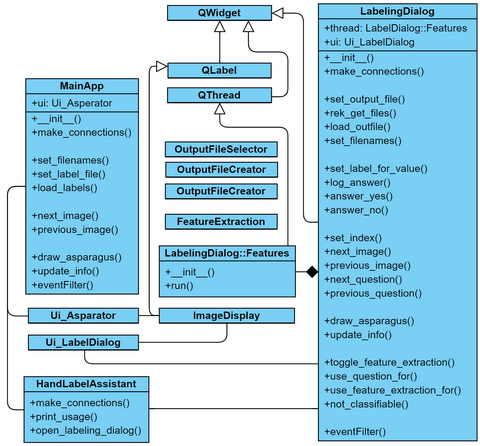
\includegraphics[scale=0.6]{Figures/chapter03/label_app_tree}
	\decoRule
	\caption[??]{??}
	\label{fig:LabelAppTree}
\end{figure}



\subsection{Manual labelling}

In this section of chapter 3, the process of manually labelling the data with the help of the hand-labelling app is laid out. It includes the sorting criteria which allocate each spear to a single asparagus class, the practice of manually labelling the preprocessed data for its features, the outcome of the labelling process, and the approach to measure the agreement of the manual labelling are described in more detail. \\
\\
The images were classified by all members of the group. As none of the group participants are experts of labelling asparagus, a general guideline for the labelling had to be established which is elaborated in detail in the following subsections. The guideline is written in accordance with the owner of the asparagus farm of Gut Holsterfeld, Mr. Silvan Schulze-Weddige. He was consulted in all questions regarding the sorting of the asparagus.
General challenges in the manual sorting in front of a computer screen, including the respective image quality, and especially the variance in the agreement of the project members were expected from the start. As the task relies on the subjective view of single humans, opinions about the affiliation to one asparagus class can diverge in critical or vague cases.  This is demonstrated in that the seasonal workers who usually sort the asparagus by hand do not agree on every case. Further, a classification session with Mr. Schulze-Weddige was held in which the project members learned to distinguish the different features that decide the class of an asparagus spear. During the session, again it emerged that some images containing critical spears - that is, where the features are not apparent - were hard to classify even by the expert. \\
To tackle the issue and to have an overview of the general agreement of the sorting between group members of the project, a measurement unit was researched and applied, namely the Kappa Agreement. It was applied on a smaller subset of pre-sorted asparagus pieces in the beginning of the manual labelling and a second time at the end of the manual sorting process. The Kappa Agreement was used to assess the degree of accordance in sorting between the single members and monitor how the sorting agreement developed during the manual labelling process. \\
\\
The first subsection, 3.4.1 Sorting criteria, expands on the guideline used for categorizing each spear of asparagus according to its features (into a single class).\\
In the second subsection, 3.4.2 Sorting outcome, the process of the manual sorting is shortly described and the achieved results are presented. \\
The ensuing third subsection, 3.4.3 Agreement measures, describes the theoretical background on the search to find a measurement for the group's agreement. \\
3.4.4 Agreement measures, focuses on the Kappa Agreement, which we chose as an evaluation measurement for the accord of our sorting, and the results of its application.


\subsubsection{Sorting criteria}

The class of an asparagus spear is decided by several factors, ranging from its shape to its colour. Put together, these single features give us the label for the spear. \\
As it was decided to label the images for their features, the features were checked by the labellers. The images were displayed with the hand-labelling app and the features are divided as follows: ‘fractured’, ‘hollow’, ‘blooming’, ‘rust on body’, ‘rust on head’, ‘bent’, ‘violet’, ‘very thick’, ‘medium thick’, ‘thick’, ‘thin’, ‘very thin’. Further, images that could not be sorted thoroughly were sorted as ‘not classifiable’ (e.g. when the spear is cut off the image). To some extent, the manual feature categorization was influenced by the price that each category of asparagus earns. High quality pieces (i.e. 1A Anna) should be thoroughly examined and sorted more conservatively. \\
In the following text, the different criteria for manually labelling the data images for their corresponding features are described. \\
 \\
Fractured \\
An asparagus spear includes the feature ‘fractured’ when it is broken, or if it does in any other way not fulfill the required length of 210 mm. \\
First, the feature was labelled manually but the procedure was abandoned shortly after because it can be derived  more precisely from the computer-vision based feature extraction ‘length’, which is automatically calculated within the labelling app. \\
It is then discerned between a fractured piece with a head and a fractured piece without a head. Whenever a spear was fractured but with the head part still attached, it was sorted like a usual, intact asparagus. However, if the head part of the spear was damaged or missing completely, no other features were chosen but the asparagus was labelled as ‘not classifiable’. \\
 \\
Hollow \\
The feature ‘hollow’ indicates that the spear is hollow inside. \\
This might be expressed by a bulgy center and a line running vertically along the spear’s body. Another, more distinct indicator is when the piece looks like two spears fused together, forming a single asparagus. A hollow asparagus can be confused with a very thick asparagus. \\
The feature can be easily checked when you have physical access to the asparagus. If the asparagus is actually hollow, it will have a hole at its bottom which you can see when turning the spear around. Unfortunately, this cannot be done when only looking at images from the side. The feature hollow sometimes even occurs without showing a clear line or obvious bulge at its center. Therefore, there is a risk of wrong classification. \\
 \\
Blooming \\
The asparagus piece is sorted as ‘blooming’ when the head part forms a recognizable flower. \\
In a blooming asparagus, a jagged pattern (slightly resembling a crown) can be seen. Also, the tip of the head part can be an indicator if it resembles a pointed cap and the petals are visible. When a spear is in full bloom, it is clearly observable. However, the distinction between a spear with clear-cut but closed petals and a spear which just started to develop a flower can be quite difficult. \\
The feature was sorted less strict in uncertain cases where the flower is not clearly distinguishable. One argument is that the flower does not develop further after the sorting process (e.g., as it happens with the feature ‘violet’). Another reason for a less conservative approach regarding the feature ‘blooming’ was to lessen any agreement errors in between the manual sorters. It was decided to sort a spear without a rather clear flower as not blooming. \\
 \\
Rust on body \\
If a spear has rust on its body, it is visible as a dark brown colour. \\
It often starts at the tips of the leaves or at the bottom part. In severe cases it spreads over the whole asparagus piece. The colour is not light brown but of a dark shade. The colour is not to be confused with bruises, pressure marks, or a slightly yellow complexion (which can occur in a mature asparagus) which are of no further concern to us.
The feature was sorted more strictly to facilitate the decision process during the manual sorting. Therefore, ‘rust’ was set to be present even when only the tip of a leaf showed a dark spot. Other brownish bruises were not classified as rust. \\
We decided to split the feature ‘rust’ into the sub-features ‘rust on body’ and ‘rust on head’. In the case of rust being only on the body, it might still be removable by peeling. If there is rust on, or very close to the head, however, it is not removable. \\
 \\
Rust on head \\
If there is a dark spot on or close to the head region recognizable as rust, it is captured by this feature. The head part is usually distinct in shape and colour from the body part of the asparagus. \\
In principle, the same guidelines applying to ‘rust on body’ can be transferred here, with an explicit focus on the top part (until around 1 cm below the collar) of the asparagus. Rust at the head can be confused with shadow caused by the petals and the luminance  of the sorting machine. Also, it might be that the head is actually violet and not rusty.
As rust at the top part of the spear cannot be removed without damaging the head, it is more decisive for the later categorization into a price class, if the head has rust. \\
 \\
Bent \\
A piece is categorized as bent, if the shape of the asparagus is curved and not straight.
Further, a spear counts as bent whenever it changes the growing direction - that is, it resembles an S curve. If it is only slightly round but can otherwise be thought of as straight and fitting next to other straight pieces without standing out, it is sorted as not being bent. If the spear looks close to the same on all three pictures, it might indicate that it is heavily bent and therefore cannot be turned on the machine’s conveyor belt. \\
Like the feature ‘blooming’, though, the feature bent has a broader range of shapes where the piece is not obviously deformed but also not completely straight. In an indecisive case, it was sorted less conservative. exception holds for S-shaped pieces, which always count as bent. \\
 \\
Violet \\
The feature ‘violet‘ indicates whether an asparagus piece is of violet colour.
The shift of colour from white to violet occurs most often around the head region - either at the tip of the head or just below the collar of the head region. As the violet complexion arises because the asparagus came into contact with sunlight, it explains why the violet colour is usually present at the top half . However, the piece can also be violet on the whole body. \\
Here, it is crucial to sort thoroughly because the spear will darken further after the sorting. Thus, even a slightly pink spear was sorted as being violet. \\
 \\
Thickness and length \\
The thickness and the length were features we did not consider recognizable by view alone (except for extreme cases). Therefore, both features were measured automatically with scripts written and implemented into the manual sorting app. The division into different categories of thickness can be inferred by the overall thickness of the spear. \\
 \\
Not classifiable \\
Whenever an image was damaged, the spear was unrecognizable, the head part of the spear was severed, two separate spears were present on one picture, the spear was cut off by the image, or other unusual circumstances on the image occured, it fell into the category of not being classifiable. The image was not further checked for its features, i.e. as bent, violet, etc., but only marked as being not classifiable.



\subsubsection{Sorting outcome}

In this section, the process and the results of the manual sorting are presented.
During the overall sorting period no major problems occurred that led to any breaks or even the abortion of the labelling process. \\
\\
Whenever an image was manually sorted in the application, the chosen labels were saved in a csv-file. As csv files are plain text files, all stored values are strings arranged in a table. The first line of the table serves as the heading, attributing each entry in the first column to a feature. As seen in Figure~\ref{fig:CSVfileOverview}, the features are noted in the first column, with the first entry being the image ID. Every feature is separated by a semicolon and can be of value 0.0, 1.0, or empty. Hence, whenever a feature was present in an image, the value was set to 1.0, while, if the feature was not present, it was marked as 0.0. However, if there was no choice in which to decide if a feature is present, no value was given to the feature. Such occurred for the case that an image was labelled as not classifiable, where all other manually selectable labels are left empty. The image path to every of the three images (a, b, and c) for one spear was also saved in the label file in the first, second and third column, respectively. \\
After the labelling process, the single csv-files with the labels were merged into one large combined\textunderscore new.csv file which was later used for the classification of the data with the different computer-vision approaches. It can be found in the study project’s Github repository under XX. \\
\\
\begin{figure}[h]
	\centering
	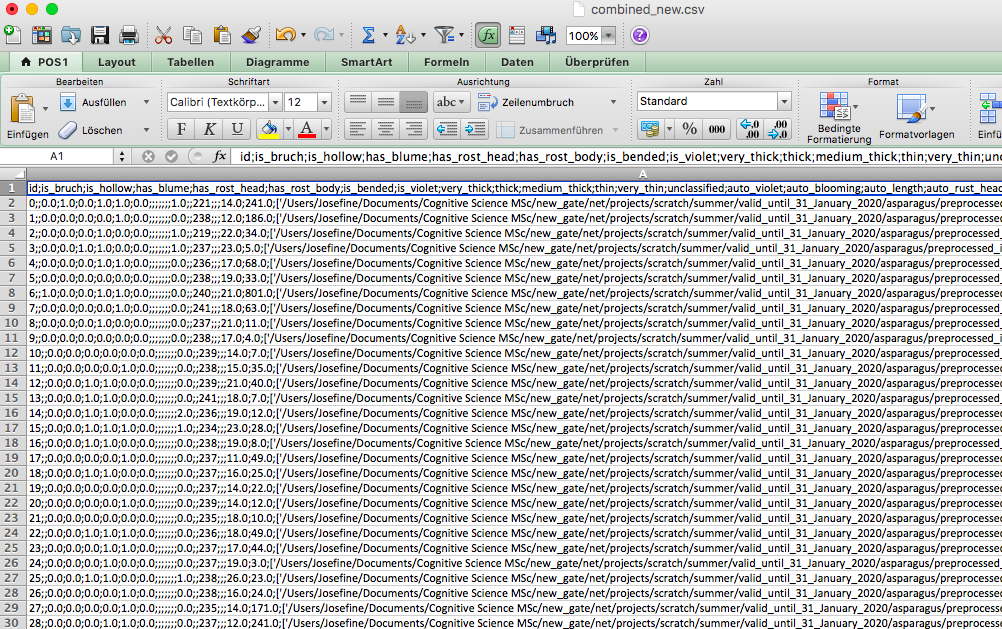
\includegraphics[scale=0.4]{Figures/chapter03/csv_overview}
	\decoRule
	\caption[CSV-File Output]{The feature labels extracted by the manual sorting process were saved in a csv file. This image shows the beginning of combined\textunderscore new.csv in which all label files were later combined.}
	\label{fig:CSVfileOverview}
\end{figure}
\\
The manual sorting lasted over the period of November 2019 to January 2020.
A session usually consisted of 500 images, with an asparagus spear being viewed in three positions from the same perspective. A session of sorting 500 images took around two to four hours. One minor factor sometimes influencing the time spent for sorting were difficulties with the external connection to the IKW store. Another factor was, of course, the large number of pictures, with some spears obviously incorporating certain features, while others needed more careful examination. The average time spent for sorting one piece (i.e. noting all features present) was around 27 - 48 seconds per spear. \\
All in all, 13319 triples of images were labelled for their features.
There is a large variation in the presence of features per image because some features were occurring more often than others. Of the acquired 13319 images, the individual features are represented as follows: 3.5\% fractured asparagus pieces, 3.3\% hollow,  12.9\% blooming, 14.7\% rust on head, 45.5\% rust on body, 40\% bent, 7.9\% violet, and 2.1\% not classifiable images. Further categories that were not manually assessed but calculated from the automatic thickness detection included 4\% very thick (i.e., above 26 mm), 29.1\% thick (20 - 26 mm), 18,7\% medium (18 - 20 mm), 17.9\% thin (16 - 18 mm), 30.3\% very thin (below 16 mm). All images that were not classifiable are excluded from the calculation of the thickness in the stated numbers.
As can be seen, many features are only sparsely present in the data. This poses an imbalance that might be relevant for later classification tasks and the usage of the dataset. \\
Further, every member of the group participated in the sorting but not everybody sorted the same number of images. Due to this circumstance, the sorting preferences of certain members are more present in the data than of others.
The manual sorting was stopped when the amount of classified data was judged to be enough by the group. \\
\\
As different people were sorting the asparagus and because the decision boundary for sorting a spear is flexible to the human eye, a measurement was needed that explores how well the members agreed in the labelling process. Thus, at the beginning and at the end of the manual labelling, images from pre-labelled classes were taken and scrutinized for their features. This was done to train the labellers but also to have a test set for the agreement measure. Every category was therefore sorted by two labellers separately and their agreement was compared. More details about the method that was chosen to assess the group’s sorting accuracy can be found in the following sections.


\subsubsection{Agreement Measures}

When different annotators label data, it is indispensable to verify the degree of agreement among raters. In order to judge how consistently the data is labeled, several statistical methods (inter-rater-reliability) can be applied. \\
 \\
For the current purpose, different agreement measures, all implemented by scikit learn, were used. The first was Cohen’s Kappa. It was chosen, as it is seen as a more robust measure than a simple agreement percentage, such as a measure of true positive and true negatives, which was traditionally used for those cases~\citep{cohen1960coefficient}. It is more robust, as the rate of agreement occurring by chance is included in the calculation. This method is applicable to compare the rating of two raters on a classification problem. This measure of agreement always lies between -1.0 and 1.0, inclusively. The higher the Kappa value, the higher the agreement. Values around 0 indicate no agreement and negative values indicate negative agreement, so to say systematic disagreement. Values between 0.41-0.6 are seen as moderate agreement, 0.61-0.8 as substantial agreement, and everything above as almost perfect agreement. Everything below 0.4 is interpreted as not acceptable (\url{https://www.ncbi.nlm.nih.gov/pmc/articles/PMC3900052/}). \\
Another statistical method used to measure agreement is the F1 score. The F1 Score is used for the evaluation of binary classification. The F1 score relies both on the precision, as well as the recall of a test’s accuracy. A F1 score value lies between 0 and 1, the higher the F1 score, the higher the agreement. \\
\\
Lastly, we looked at the accuracy measure. For a normalized accuracy score, the values lie between 0 and 1, and the best performance is 1. This measure returns the fraction of correctly classified samples. It is a less robust measure than Cohen’s Kappa score.

\subsubsection{Reliability}

In order to evaluate the degree of agreement of our data, we made agreement measures at two points in time (for our API documentation see: \url{https://asparagus.readthedocs.io/en/latest/api/measure\textunderscore agreement.html}). The first time, six different annotators labelled images out of each asparagus group (13 groups). We ensured that always two different annotators labelled the same set of images. Results were not as good as hoped for. The Kappa scores varied strongly between groups and features from -0.03 to 0.76, while the accuracy scores ranged from 0.49 to 1. It seemed untypical to us, that the agreement scores were so low, even though the raters give the same label to many of the asparagus pieces. This is a known problem~\citep{powers2012problem} ~\citep{sim2005kappa} ~\citep{feinstein1990high}(\url{https://www.sheffield.ac.uk/polopoly\textunderscore fs/1.404095!/file/RSS\textunderscore Poster\textunderscore Laura\textunderscore Flight\textunderscore Final.pdf}). \\
\\
\begin{figure}[h]
	\centering
	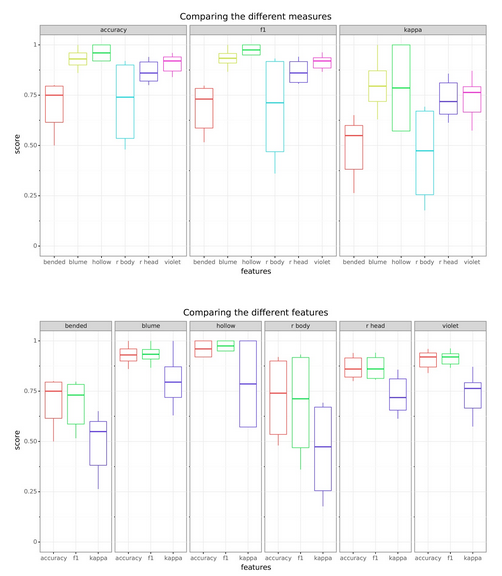
\includegraphics[scale=0.6]{Figures/chapter03/kappacompare}
	\decoRule
	\caption[Comparing the different features]{All scores are aggregated scores over all annotator pairs. The first plot shows the results agreement measure-wise, the second plot feature-wise.}
	\label{fig:KappaCompare}
\end{figure}

One reason for our results could be that we compared the agreement group-wise. This means that we already knew in advance that for certain features, we have almost only 1s or almost only 0s for all images of one group. For Kappa scores, if the distribution of 0s and 1s is not balanced, disagreement of the underrepresented value is punished more heavily. Therefore, we decided to repeat our agreement measure and do it this time feature-wise on non-labeled images, so that the annotators could not anticipate a specific group label. In order to better understand the reliability of our data, we also decided to look at the accuracy score and the F1 score, additionally. Before we did so, we labeled another 50 images all together, clarified classification boundaries again and discussed unclear images. \\
\\
The second time, 50 images were labeled by 4 annotators. The agreements were measured annotator-pair-wise, and then averaged. The results in the Cohen’s Kappa score vary between and within features, and also between annotator pairs. However, the results are much better than the first time. The highest aggregated kappa score over all annotator pairs is reached for the feature flower (0.79), then hollow (0.79), violet (0.76), rusty head (0.72), bent (0.55) and lastly for rusty body (0.47).
For the features flower, rusty head and violet, the IQR is quite small (), whereas the IQR for hollow, bent and rusty body is much larger (). \\
\\
The agreement scores accuracy and F1 yielded very similar results. Results were slightly better than the Kappa scores, in total and  for each feature. The highest accuracy score is reached for the feature hollow (0.96), then flower (0.93), then violet (0.92), then rusty head (0.86), then bent (0.75) and then rusty body (0.74). The order is the same for the F1 scores. The median F1 scores lie between (0.71 and 0.97). \\
\\
All in all, one can therefore say that the agreement scores indicate moderate up to substantial agreement. Agreement is highest for the features flower, violet and rusty head.


\subsection{The asparagus dataset}

TODO: Any information on the data we worked with for our approaches.


\subsubsection{Different datasets}

TODO \\
\\

What exists:
\begin{itemize}
\item Raw data (reading functions)
\item Numpy Array
\item TFRecord
\item Tf.data.Dataset
\item Other dataformats: \url{https://github.com/tensorflow/io}
\item Publication -> Tf.data.dataset / tf.dataset
\end

Best practice:
\begin{itemize}
\item Theoretical
\end{itemize}

 
Used on our data:
\begin{itemize}
\item Difficulties
\begin{itemize}
\item Mulitlabel
\item Semisupervised dataset – not all labelled
\item Misunderstandings
\end{itemize}
\item Results & Discussion
\end{itemize}

Summary
\begin{itemize}
\item Theoretical usage on our data   
\item Implementation in our repo
\item How to use in future work
\end{itemize}

\begin{figure}[h]
	\centering
	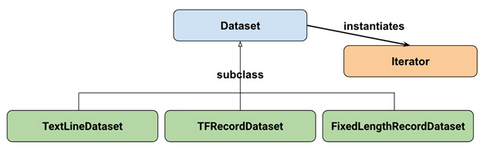
\includegraphics[scale=0.6]{Figures/chapter03/dataset_tf}
	\decoRule
	\caption[Tensorflow Dataset]{The tf.dataset.}
	\label{fig:DatasetTF}
\end{figure}

\begin{figure}[h]
	\centering
	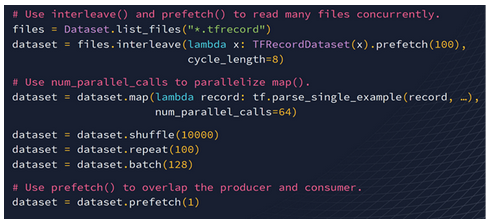
\includegraphics[scale=0.6]{Figures/chapter03/dataset_code}
	\decoRule
	\caption[??]{??}
	\label{fig:DatasetCode}
\end{figure}


Additionally, we created a single numpy dataset for the labelled images that could be easily stored and loaded for training. Firstly, all the identification numbers from the labelfiles were selected and the corresponding images were found and copied to a separate folder. This folder contains all the images for which we have labels. Secondly, the images were grouped by their identification number, which means the three perspectives of each asparagus spear were combined. We decided to downsample the images for creating this dataset to facilitate the training process and reduce memory consumption. Initially, each image was downsampled by a factor of six, that means every 6th pixel was used in the reduced image, but this factor can be easily changed and a new dataset will be created for the individual needs of each approach. After that they were transformed to a numpy array and concatenated to a single file. The images were either concatenated horizontally, so that in the resulting image the three perspectives appear to lay next to each other, or vertically, so that the images are stacked one after another. Finally, all the concatenated arrays were combined to a single four dimensional dataset. The first dimension depicts the number of labelled asparagus spears, the second and third dimension represent the height and the width of the images, respectively.  Further, the fourth dimension represents the depth, which is three for the horizontally concatenated images, namely the RGB values, and nine for the vertically stacked images.


\subsubsection{Challenges}

Problems and challenges during the creation of the datasets.

\begin{itemize}
\item What were the challenges in creating a general dataset?
\item What were challenges in general?
\item How well could we work with the datasets?
\item What was used as training data, validation data, and test data?
\end{itemize}

%----------------------------------------------------------------------------------------
%	CLASSIFICATION OF DATA VIA DIFFERENT METHODS
%
%	Classification of the data using different approaches.
%----------------------------------------------------------------------------------------
\section{Classification}
\label{ch:Classification}

Given the structure of our data set, different machine learning and computer vision methods were chosen to tackle the problem of image classification.

\bigskip
Image classification refers to the method of identifying to which category an image belongs to, according to its visual information. Classification problems can be divided into three different types: binary, multiclass and multi-label. Moreover, there are different methods on how to approach image classification. Those can be divided into three main groups: supervised learning, semi-supervised learning and unsupervised learning~\citep{har2003constraint}.

Binary classification can be used to decide whether a certain feature is present or not. Multiclass classification solves this problem as well, but is also applicable to data with more than two classes. As the class label results from a combination of the presence of certain features and the absence of others, it is also reasonable to go for a multi-label classification approach. In this approach, several features are learned simultaneously without being mutually exclusive.

During our group work, algorithms of the different classification types as well as of the different learning types were applied.
In the long run, an integrated model was aimed at predicting all features of a single asparagus spear, from which the final class label can be inferred. However, as intermediate steps towards that goal, the focus was to optimize models on identifying the presence of the features described in~\autoref{sec:AutomaticFeatureExtraction}.

\bigskip
This chapter gives a general background of the different approaches chosen for our image classification problem, as well as a detailed overview of the concrete implementations of the models and the mechanisms of their hyperparameters.


\subsection{Supervised learning}
\label{sec:SupervisedLearning}

In machine learning, there are different approaches for an application to be trained on a set of data~\citep{geron2019hands,bishop2006pattern}. Depending on the level of supervision that the system receives during the training phase, the learning process is grouped into one of three major categories~\citep{geron2019hands}. One of these categories is supervised learning. For supervised learning approaches, the training data includes not only the input but also its corresponding target labels. The objective is to find a mapping between object \((x)\) and label \((t)\) when a set of both \((x,t)\) is provided as training data to the application~\citep{olivier2006semi}. An advantage of supervised learning is that the problem is well defined and the model can be evaluated in respect to its performance on labeled data~\citep{daume2012course,olivier2006semi}. In other words, the labels are used as a direct basis for the model’s optimization function during training.

Supervised learning spans over a large set of different methods, from decision trees and random forests, to \acrfullpl{svm}  and \acrlongpl{ann}~\citep{caruana2006comparison,geron2019hands}.

A classical task for supervised learning systems is the classification of received data which means  mapping the input data to one of a finite number of categories~\citep{bishop2006pattern}.
The disadvantage of supervised learning is the effort of receiving enough labeled data. It can be challenging to obtain fully labeled data of high quality~\citep{zhu05survey,figueroa2012predicting}.

\bigskip
In the following sections, different supervised learning methods were implemented to solve the classification task using the data that was manually labeled for features as described in~\autoref{ch:Dataset}. In \ref{subsec:FeatureEngineering}~\nameref{subsec:FeatureEngineering}, an approach using an \acrshort{mlp} is described for feature classification. The section of \ref{subsec:SingleLabel}~\nameref{subsec:SingleLabel} is concerned with labeling the input images with a \acrshort{cnn} in a binary setup for their designated features. In section \ref{subsec:MultiLabel}~\nameref{subsec:MultiLabel}, a neural network is trained on the data to label it not only for one feature but all features at the same time. In the fourth section, \ref{subsec:HeadNetwork}~\nameref{subsec:HeadNetwork}, a \acrshort{cnn} is used to train solely on the head image data for the features flower and rusty head.
Finally, in \ref{subsec:FeaturesToLabels}~\nameref{subsec:FeaturesToLabels}, a random forest approach is described to map the features of the image data to their class label.


\subsubsection{Prediction based on feature engineering}
\label{subsec:FeatureEngineering}

Besides approaches that directly use images as an input one may use high level feature engineering. That is, one can retrieve sparse representations that contain relevant information in a condensed form and apply classical machine learning classifiers such as \acrshortpl{mlp} to predict labels~\citep{zheng2018feature}. Note that we use the ambiguous term MLP in the strict sense i.e.\ for networks that comprise fully connected layers only and speak of CNNs if the network contains one or more convolutional layers. As we used MLPs for sparse features and CNNs for images we oppose these typical approaches for the respective domains of data.  \acrshortpl{mlp} classifiers for sparse features are considered comparatively simple as only few network hyperparameters have to be defined and typically comprise a limited number of neurons (see below). Besides retrieving sparse features can make the learning task very simple and allows for a higher degree of control over what is measured.

The simplicity of shallow \acrshortpl{mlp} means that the best suitable structure could be found more easily as compared to deep learning \acrshortpl{cnn} that require a special structure to address the vanishing gradient problem and have many other hyperparameters such as the size and number of kernels~\citep{wang2019vanishing}.  As a consequence, finding suitable hyperparameters for \acrshortpl{mlp} (i.e.\ the number of hidden layers and neurons per layer) is comparatively easy.\footnote{The challenge of finding appropriate network parameters is well known in the deep learning community: \enquote{Designing and training a network using backprop requires making many seemingly arbitrary choices $[...]$. These choices can be critical, yet there is no foolproof recipe for deciding them because they are largely problem and data dependent}’~\citep[p.~9]{lecun2012efficient}. The requirement to specify hyperparameters is a disadvantage of neural networks (including \acrshortpl{mlp}) as compared to parameter free methods~\citep{scikit2019neural}. Due to the combinatorial explosion, the challenge of finding suitable parameter settings is harder for more complex networks as more options must be considered.} This is beneficial because underfitting can potentially be due to an unsuitable network design ~\citep{lecun2012efficient}. 

An extensive search in hyperparameter space is possible for simple \acrshortpl{mlp} for sparse features, because they have few network hyperparameters and because networks for training on sparse representations typically have a limited number of neurons. This becomes clear in our example of learning the binary feature curvature using 18 partial angles as the input. The dimensionality of the input layer of networks that are trained on dense features (here: three images of size $1040\times1376$ with three color channels i.e.\ more than twelve million values) are substantially larger. The reduced dimensionality of sparse features could even be considered as the defining criterion for the term. For our example, a network that uses the raw input requires an input layer with more than twelve million neurons as compared to only 531 neurons in the whole  \acrshortpl{mlp} for partial angles. Taken together this results in fast training of a network that is trained on sparse features - typically a MLP \footnote{MLPs can be used for sparse data because there is no necessity to further limit the size of  the network by use of convolutional layers and it is not always the case that a locality criterion holds.}. This allows for many experiments to find best suitable network hyperparameters. 

The use of \acrshortpl{mlp} in combination with feature engineering certainly also has drawbacks as compared to the direct application of deeper  \acrshortpl{cnn}. Most strikingly one is at risk of discarding relevant information when defining the features and has to find and implement ways to reliably measure them. Because of the benefits we nonetheless tested the performance of shallow \acrshortpl{mlp} using color histograms and partial angles of asparagus spears.\footnote{~See \url{https://github.com/CogSciUOS/asparagus/tree/FinalProject/classification/supervised/mlps\_and\_feature\_engineering} (as of 11/27/2020)}

\bigskip
\textbf{Violet and rust prediction based on color histograms} 

The feature violet is based on the distribution of sufficiently intense color hues in the violet color range. The initial approach of automatically measuring the feature as described in ~\autoref{sec:AutomaticFeatureExtraction} faces at least two drawbacks. First, it requires defining two thresholds. Second, the impression of a violet asparagus spear could possibly be affected by the combination of colors that are potentially outside the violet range or that are too pale to be considered (see~\autoref{subsec:Violet}). The same holds for the features rusty body and rusty head. Hence, in a second approach histograms were computed for foreground pixels after transforming the images to palette images with 256 color hues (see \autoref{sec:Preprocessing}). The resulting representation is a sparse descriptor that allows to predict color features using explicitly defined rules or trainable machine learning models.

\begin{figure}[!htb]
	\centering
	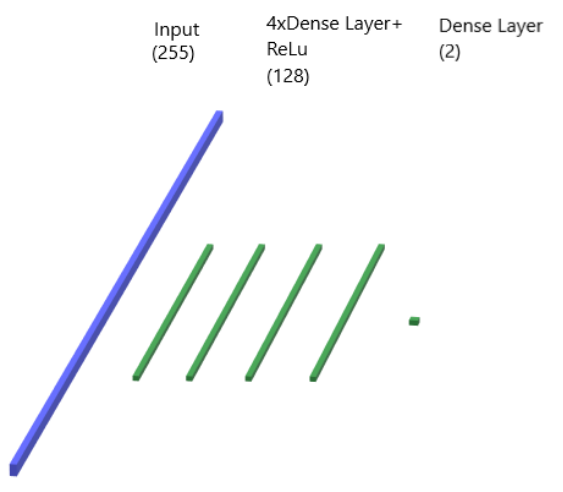
\includegraphics[width=0.70\textwidth]{Figures/chapter04/fe_color.png}
	\decoRule
	\caption[Feature Engineering Net Structure Color]{\textbf{Feature Engineering Net Structure Color}~~~The depiction shows the network structure of the \acrshort{mlp} for color-related features.}
	\label{fig:FeatureEngineeringNetStructureColor}
\end{figure}

\begin{table}[!h]
	\centering
	\resizebox{\columnwidth}{!}{%
	\begin{tabular}{lrrrrrr}
		{} &  False positive &  False negative &  True positive &  True negative &  Sensitivity &  Specificity \\
		\noalign{\smallskip}
		\hline
		\noalign{\smallskip}
		violet     &            0.04 &            0.03 &           0.05 &           0.88 &         0.62 &         0.96 \\
		rusty body &            0.19 &            0.14 &           0.33 &           0.34 &         0.71 &         0.65 \\
		\noalign{\smallskip}
		\hline
	\end{tabular}%
	}
	\caption[Feature Engineering Color-Histogram-Based Prediction]{\textbf{Feature Engineering Color-Histogram-Based Prediction}~~~Performance of color histogram-based predictions with a \acrshort{mlp}.}
	\label{tab:performance_color_feature_based}
\end{table} 

\begin{figure}[!htb]
	\centering
	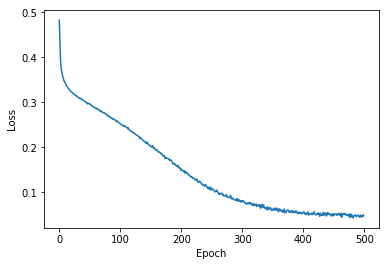
\includegraphics[scale=0.7]{Figures/chapter04/fe_palette_color.png}
	\decoRule
	\caption[Feature Engineering Learning Curve for Palette-Color Histogram based Prediction]{\textbf{Learning Curve for Palette-Color Histogram based Prediction}~~~The depiction shows the loss per training episode for the \acrshort{mlp} trained on histograms of palette images.}
	\label{fig:FeatureEngineeringPaletteColor}
\end{figure}

The sample set contains a histogram for each labeled asparagus. Twenty percent are randomly assigned to the evaluation set. A simple \acrshort{mlp} with four hidden layers and 128 neurons in each of them was trained on the resulting normalized histograms of palette colors (ReLU activation / sigmoid activation in the final layer). Hyperparameters were optimized and the network was trained for a total of 500 epochs as the learning curve indicates convergence at this point.

\bigskip
\textbf{Curvature prediction based on partial angles} 

The sensitivity for curvature detection is high: 82\% of all bent spears were identified as such. In comparison, this holds for 71\% of the spears affected by rust and for 62\% of the violet spears. In contrast, almost all spears that are identified as not to be violet are labeled accordingly (96\% specificity). However, the specificity for rust (65\%) and curvature (67\%) is lower. Although the accuracies are far from perfect the results appear to be promising.

\begin{figure}[!htb]
	\centering
	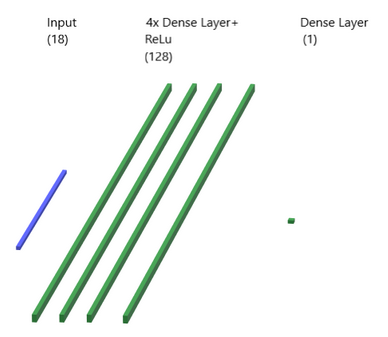
\includegraphics[width=0.70\textwidth]{Figures/chapter04/fe_curvature.png}
	\decoRule
	\caption[Feature Engineering Net Structure Curvature]{\textbf{Feature Engineering Net Structure Curvature}~~~The depiction shows the network structure of the \acrshort{mlp} for the feature bent.}
	\label{fig:FeatureEngineeringNetStructureCurve}
\end{figure}

The receiver operating characteristic reveals that the prediction is of better quality for violet and curvature prediction as compared to rust prediction which is reflected in a smaller area under the curve for the latter. Possibly this reflects that rather small brown spots were considered rust by some raters but not by others. 

\begin{table}[!h]
	\centering
	\resizebox{\columnwidth}{!}{%
	\begin{tabular}{lrrrrrr}
		{} &  False positive &  False negative &  True positive &  True negative &  Sensitivity &  Specificity \\
		\noalign{\smallskip}
		\hline
		\noalign{\smallskip}		
		bent &            0.19 &            0.07 &           0.34 &            0.4 &         0.82 &         0.67 \\
		\noalign{\smallskip}
		\hline
	\end{tabular}%
	}
	\caption[Feature Engineering Curvature Prediction]{\textbf{Curvature Prediction}~~~Performance of curvature prediction based on angles.}
	\label{tab:performance_angle_based}
\end{table}

Considering the low agreement in labeling, high values for the specificity and sensitivity of the classifier are not expected. A likely explanation for rather low values is that the model generalizes deviating and potentially contradicting perceptual color-concepts that we had when attributing labels. Arguably, only little information was discarded by computing the sparse representations that served as an input for training. However, information about irregularities in the outline are not reflected in the partial angles but might contribute to the perception of curvature. The same holds for the spatial distribution of colored pixels which might contain additional information regarding the detection of rust and violet. Nonetheless, the major criteria are captured. As \acrshortpl{mlp} are suitable to establish non-linear mappings and as the task of mapping high level features (such as partial angles) to human estimates appears to be rather simple, one may speculate that there is rather little potential to improve the predictive quality using other techniques. By introducing a bias, the sensitivity of the classifier can be adjusted at the cost of more false positives. Here, introducing a bias means that the threshold that is used to convert the floating point outputs of a neural network to booleans that indicate whether a feature is present or not is set to values other than 0.5. The possibility of making the classifier more or less sensitive appears to be a good option to be implemented as a feature for customization by the user in asparagus sorting machines.

\begin{figure}[!hb]
    \centering
    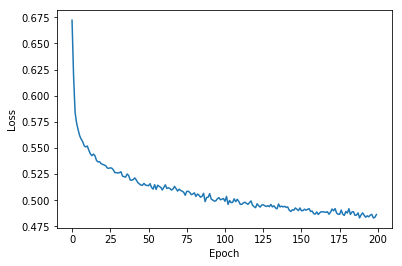
\includegraphics[scale=0.7]{Figures/chapter04/fe_curve.png}
    \decoRule
    \caption[Feature Engineering Learning Curve For Angle Based Prediction]{\textbf{Learning Curve For Angle Based Prediction}~~~The depiction shows the loss per training episode for the \acrshort{mlp} trained on partial angles of the centerline of asparagus spears.}
    \label{fig:FeatureEngineeringCurve}
\end{figure}

\begin{figure}[!htb]
    \centering
    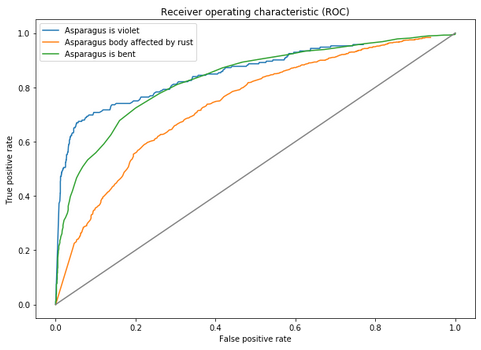
\includegraphics[scale=0.6]{Figures/chapter04/fe_roc.png}
    \caption[Feature Engineering ROC Curve]{\textbf{ROC for MLPs Trained on High Level Features}~~~The depiction shows the \acrfull{roc} for the classifiers that were trained on the features retrieved via feature engineering with \acrshortpl{mlp}. This allows for comparison of the performance. A larger area under the \acrshort{roc} curve indicates better performance while a curve close to the diagonal line indicates poor results.}
    \label{fig:FeatureEngineeringROC}
\end{figure}


\subsubsection{Single-label classification}
\label{subsec:SingleLabel}

In the following chapter, a \acrlong{cnn} is described, which is used for single-label classification on features.\footnote{It can be found at \url{https://github.com/CogSciUOS/asparagus/tree/FinalProject/classification/supervised/single-label-CNN} (as of 11/27/2020).} The approach was tested on the 13319 hand-labeled data images. 13 models were created, each predicting one feature.~\footnote{The 13 features to predict are: fractured, hollow, flower, rusty head, rusty body, bent, violet, very thick, thick, medium thick, thin, very thin, and not classifiable.}

A general model structure was needed as inspiration for the \acrshort{cnn}. For example, the \acrfull{vgg}~networks with varying depth seem to be a good choice for image classification as their \acrshort{vgg}16 won the ImageNet challenge of 2014 and is often implemented for image classification tasks~\citep{hassan2018vgg,vgg2014original}. However, there are two major drawbacks to using them. That is, they are slow to train and in need of a lot of memory storage due to their depth and the amount of fully-connected layers \citep{hassan2018vgg,zhang2015accelerating}. Part of these problems also arise with even deeper networks like ResNet~\citep{resnet2016original,hassan2019resnet}. Thus, AlexNet is chosen as a blueprint for the \acrshort{cnn} because it is small in relation to other networks while still performing comparatively good~\citep{hassan2019alexnet,alexnet2012original,geron2019hands}. As the variance in the data images is relatively small it is assumed that a smaller number of layers is sufficient as compared to deeper networks like \acrshort{vgg}~\citep{geron2019hands}.

\begin{figure}[!htb]
	\centering
	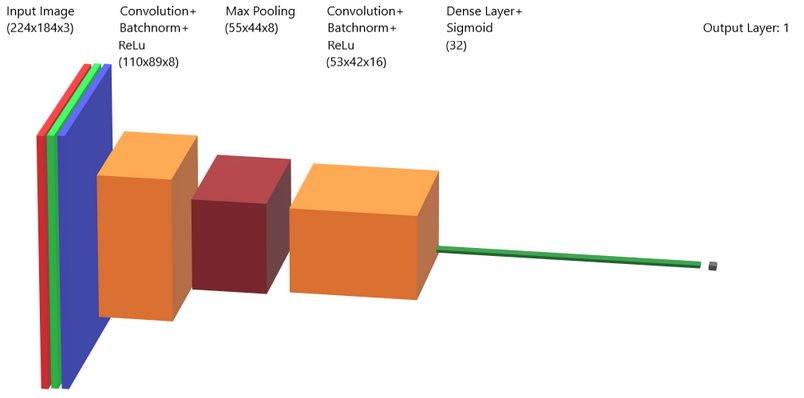
\includegraphics[width=0.95\textwidth]{Figures/chapter04/singleCNN_net_structure.png}
	\caption[Single-Label CNN Net Structure]{\textbf{Single-Label CNN Net Structure}~~~The depiction shows the network structure of the simple feedforward \acrshort{cnn}.}
	\label{fig:SingleLabelNetStructure}
\end{figure}
 
\bigskip
The network comprises four hidden layers: a convolutional layer, followed by a pooling layer, a second convolutional layer, and a dense layer. The input is an array of multiple horizontally stacked images with background and reduced by a factor of six. This input is trained on a set of binary labels containing information on whether the respective feature label applies to the current image. The output of the network gives a prediction on each entered image gated by a sigmoid function on a range between zero and one. The rounded integer values of this output give a prediction of the apparent feature label.
For the training phase of the model, the Adam optimizer is used because of its general acceptance as the state of the art optimizer for backpropagation~\citep{bushaev2018adam,kingma2014adam}. As a loss function, binary cross-entropy is used as it promises good results for binary single-label classification tasks~\citep{geron2019hands,godoy2018understanding,dertat2017applied}.
 
When training \acrlongpl{ann}, it can be difficult to find clear guidelines on how to implement an architecture such that an optimal training performance is given~\citep{heaton2015aifh,geron2019hands,bettilyon2018classify}. Hence, the idea was to start with the simplest form of a \acrshort{cnn} and then gradually increase the complexity of the network. While AlexNet provides a good baseline for an image classification network, its architecture is still assumed to be unnecessarily complex for the given task. First, the architecture was reduced to the minimum number of layers and parameters needed for a \acrshort{cnn}. Over the period of training optimization, various processing steps and hyperparameters were implemented and compared according to their performance. During this process, the data was split between 12000 samples for training data and 1319 samples for validation data in order to have a reasonable overview on the possible test performance and to directly check for overfitting. The data used as test data was randomly chosen from the whole data set.\footnote{Only the models trained on detecting the features hollow, flower, rusty head, rusty body, bent, and violet use the same validation set. Like this, a better comparison can be made between them. For the other features, the validation set was always randomly composed anew before model training.}

\bigskip
In the following, the development of the hyperparameters over time is explained.
 
The batch size was initiated comparatively low with 64 samples per batch but soon adjusted to a value of 512 samples. The larger batch size was implemented in order to guarantee the convergence of the training data, since smaller batch sizes result in jumping gradients, which are not able to converge into any minimum~\citep{bengio2012practical}.
 
Various learning rates were tested during the optimization process. The initial learning rate of 0.003 (which is the standard learning rate for Adam optimizers in TensorFlow~\citep{kingma2014adam,geron2019hands}) was soon found to be too large to guarantee convergence of the algorithm. Thus, the learning rate was decreased and found to be most effective in the range of \(1e^{-5}\) to \(1e^{-8}\). A gradually decreasing learning rate was tested in order to make the training more effective~\citep{bengio2012practical}.~\footnote{In theory, the Adam optimizer already manages learning rate decay~\citep{kingma2014adam}.} It does not yield better results and thus a constant learning rate of \(1e^{-5}\) is implemented.
 
Starting with the smallest layer size possible, in the course of time more layers were added. For example, in order to detect the feature fractured one layer for the edge detection is considered to be sufficient. For other, higher-level features, such as bent, additional convolutional layers were expected to be more helpful~\citep{geron2019hands}. During the training process, it was settled to a model with the architecture described above.
 
A small number of kernels is used compared to AlexNet since for single-label classification fewer kernels are expected to be needed \citep{geron2019hands}. The kernel size is picked to be eight~$5\times5$ kernels for the first convolutional layer and 16~$3\times3$ kernels for the second convolutional layer. The hidden dense layer consists of 32 neurons. These sizes are assumed to be sufficient, since increasing the number of kernels does not lead to any better results but to overfitting on the training data.
 
Both convolutional layers of the model are built with batch normalization. The gradients were inspected visually and the results give no reason for assuming exploding or vanishing gradients~\citep{pascanu2012understanding}.
 
A next step was to weight the loss function because of the largely unbalanced data~\citep{he2009learning,batista2004study}. However, this did not lead to any changes. The model still tended to make an unbalanced prediction by classifying all values as negative samples. Another idea is to reduce the data set to make the number of images with the regarding feature present even to the number of images where it is absent. This would mean to throw away valuable data, which can otherwise provide information about negative cases to support the model in its training~\citep{batista2004study}. It was decided to keep all images and instead balance the data by multiplying the minority of samples to match the number of contrary samples. As there was no feature positively exceeding a presence of 50\% in the data, solely positive labels were oversampled. The balancing was only performed on the training data, while the test data was not changed.
 
To prevent overfitting of the negative data samples, \(L_2\) regularization was applied.
 
To improve training performance, different kinds of data augmentation were tested \citep{brownlee2019augmentation} like horizontal flipping or small changes in the angle (up to 5\textdegree ) but not used in the final version.

\bigskip
Around 2700 to 5400 training steps are performed for the training, translating roughly to 120 epochs (with an exception for the model of feature fractured, which is trained for 60 epochs). Due to the balancing of the data, the number of training data (and therefore the ratio of training steps to epochs) varied when training the \acrshort{cnn} on the different features.

\begin{table}[h]
	\centering
	\resizebox{\columnwidth}{!}{%
	\begin{tabular}{llllll}
		{} & Sensitivity & Specificity & Validation Accuracy & Balanced Accuracy & Training Steps \\
		\noalign{\smallskip}
		\hline
		\noalign{\smallskip}
		fractured & 0.8846 & 0.9976 & 99.32\% & 94.11\% & 2690 \\
		\smallskip
		hollow & 0.7308 (0.7692) & 0.9821 (0.9831) & 97.58\% (97.77\%) & 85.65\% (87.62\%) & 5390 (4270)  \\
		\smallskip
		flower & 0.5603 (0.6983) & 0.8975 (0.8288) & 85.96\% (81.41\%) & 72.89\% (76.36\%) & 4790 (2900) \\
		\smallskip
		rusty head & 0.4311 (0.5210) & 0.8695 (0.8106) & 79.86\% (76.38\%) & 65.03\% (66.58\%) & 4670 (3320) \\
		\smallskip
		rusty body & 0.6420 (0.6400) & 0.7767 (0.8049) & 71.15\% (72.51\%) & 70.94\% (72.25\%) & 2990 (2270) \\
		\smallskip
		bent & 0.6541 (0.6753) & 0.7533 (0.7500) & 71.25\% (71.93\%) & 70.37\% (71.27\%) & 3230 (2470) \\
		\smallskip
		violet & 0.4643 (0.5119) & 0.9652 (0.9452) & 92.45\% (91.00\%) & 71.48\% (72.86\%) & 5150 (3550) \\
		\smallskip
		very thick & 0.9778 & 0.9939 & 99.32\% & 98.59\% & 5390 \\
		\smallskip
		thick & 0.9525 & 0.9688 & 96.41\% & 96.07\% & 3950 \\
		\smallskip
		medium thick & 0.8917 & 0.9249 & 91.87\% & 90.83\% & 4550 \\
		\smallskip
		thin & 0.9399 & 0.9280 & 93.13\% & 93.40\% & 4190 \\
		\smallskip
		very thin & 0.9733 & 0.9579 & 96.13\% & 96.56\% & 4310 \\
		\smallskip
		not classifiable & 0.5217 & 0.9961 & 98.79\% & 75.89\% & 5390 \\
		\noalign{\smallskip}
		\hline
	\end{tabular}%
	}
	\caption[Single-Label CNN Classification Results]{\textbf{Single-Feature Label Classification Results}~~~In this table, the sensitivity, specificity, validation accuracy, balanced accuracy, and the number of training steps are given for each feature model after training on 12000 hand-labeled data images. The numbers in brackets indicate the best result for the model in relation to its balanced accuracy. For most features, training lasted for 120 epochs. However, the number of data samples (and thus training steps) varies between features because of the data balancing.}
	\label{tab:SingleLabelResults}
\end{table}
 
\begin{figure}[!htb]
	\centering
	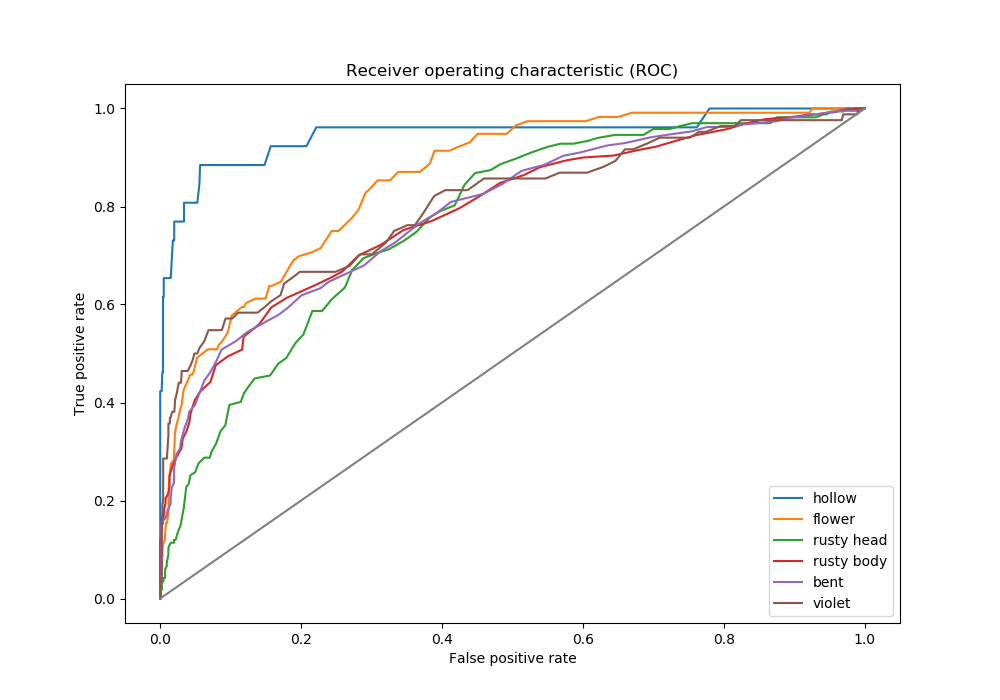
\includegraphics[scale=0.6]{Figures/chapter04/singellabelROC.png}
	\decoRule
	\caption[Single-Label CNN ROC Curve]{\textbf{ROC Curves for Six Feature Models}~~~The figure shows the \acrshort{roc} curves for the six models trained to detect the features hollow, flower, rusty body, rusty head, bent, and violet, respectively. For the features rusty body and bent, the curve is comparatively smooth as their representation is more balanced. The curves are calculated from 1319 data samples.}
	\label{fig:SingleLabelROC}
\end{figure}

The \acrshort{cnn} is trained on 13 features separately, resulting in 13 trained models. For some features, there are no labels in the csv-file but they can be calculated from the parameters length and width of an asparagus. That is, the features very thick, thick, medium, thin, and very thin are all calculated from the thickness measured by the automatic feature extraction algorithm for width, according to the boundaries for each class label (for reference, see \autoref{tab:AsparagusLabels} and \autoref{fig:LabelTree} in \autoref{sec:BackgroundSortingAsparagus}, and also \autoref{subsec:Width}). For the feature fractured, the length was set to a threshold of 210 mm, with all asparagus of smaller length labeled as fractured. Additionally, asparagus labeled as not classifiable was included for training the model that is detecting the feature fractured. The reason is that fractured asparagus without a head part was previously labeled as not classifiable (see the feature descriptions in \autoref{subsec:Length}). The feature not classifiable was also trained on separately. Further, for all other features, not classifiable samples were removed before training to prevent a bias in the occurrence of false positives.

\begin{figure}[!htb]
	\centering
	\begin{subfigure}{0.3\textwidth}
		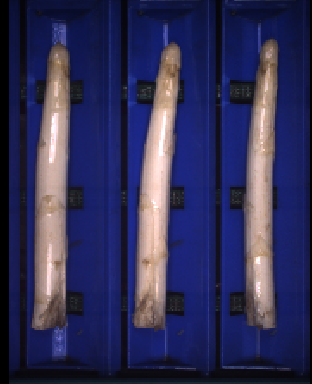
\includegraphics[width=0.9\linewidth]{Figures/chapter04/hollow_falsenegative_01.png}
		\vspace{-5pt}
		\caption{False Negative}
	\end{subfigure}
	\begin{subfigure}{0.3\textwidth}
		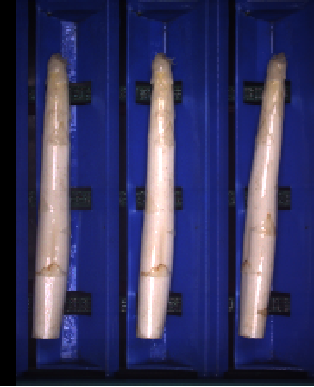
\includegraphics[width=0.9\linewidth]{Figures/chapter04/hollow_falsenegative_02.png}
		\vspace{-5pt}
		\caption{False Negative}
	\end{subfigure}
	\begin{subfigure}{0.3\textwidth}
		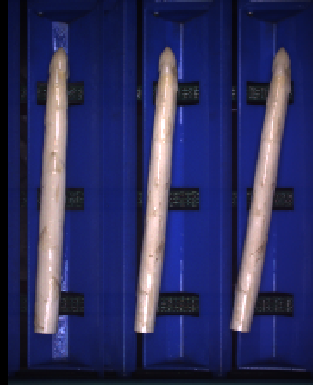
\includegraphics[width=0.9\linewidth]{Figures/chapter04/hollow_falsenegative_03.png}
		\vspace{-5pt}
		\caption{False Negative}
	\end{subfigure}

	\begin{subfigure}{0.3\textwidth}
		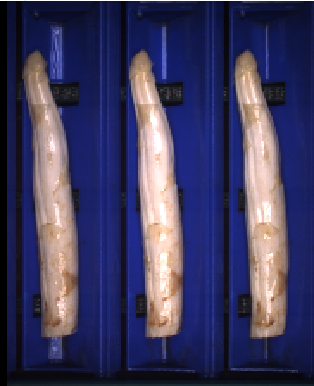
\includegraphics[width=0.9\linewidth]{Figures/chapter04/hollow_falsepositive_01.png}
		\vspace{-5pt}
		\caption{False Positive}
	\end{subfigure}
	\begin{subfigure}{0.3\textwidth}
		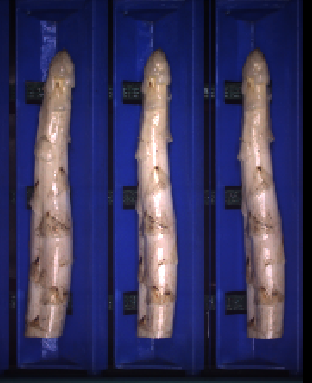
\includegraphics[width=0.9\linewidth]{Figures/chapter04/hollow_falsepositive_02.png}
		\vspace{-5pt}
		\caption{False Positive}
	\end{subfigure}
	\begin{subfigure}{0.3\textwidth}
		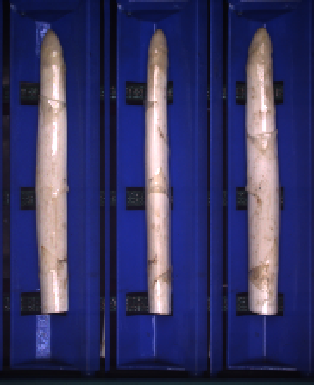
\includegraphics[width=0.9\linewidth]{Figures/chapter04/hollow_falsepositive_03.png}
		\vspace{-5pt}
		\caption{False Positive}
	\end{subfigure}
	\vspace{-5pt}
\caption[Single-Label CNN Example Images Feature Hollow]{\textbf{Feature Hollow}~~~Randomly chosen example images of false negatives and false positives of the feature hollow after 5400 training steps. Image (A) and (C) might have been sorted wrongly as the presence of the feature hollow is not obvious. Of the false positives, image (E) might have also been sorted wrongly, as the vertical line can be seen on the lower part of the asparagus which is a sign for a hollow asparagus (for reference, see the section \nameref{subsec:Hollow}). The thickness of the asparagus might have been an indicator to the model that the feature is present. This can be seen in image (D) which shows a thick asparagus, and image (F) where the asparagus' thickness varies depending on its position.}
    \label{fig:ExampleImagesHollow}
\end{figure}

\begin{figure}[!htb]
	\centering
	\begin{subfigure}{0.3\textwidth}
		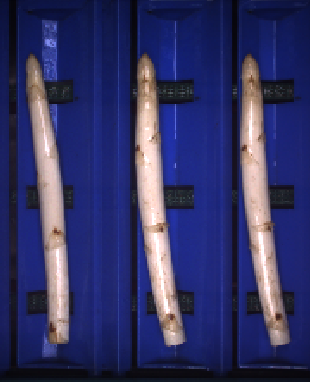
\includegraphics[width=0.9\linewidth]{Figures/chapter04/bent_falsenegative_01.png}
		\vspace{-5pt}
		\caption{False Negative}
	\end{subfigure}
	\begin{subfigure}{0.3\textwidth}
		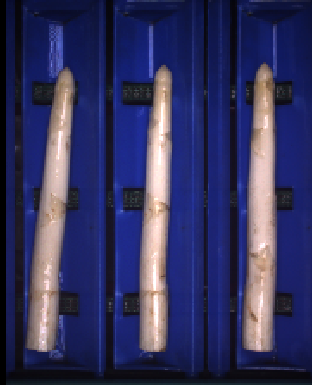
\includegraphics[width=0.9\linewidth]{Figures/chapter04/bent_falsenegative_02.png}
		\vspace{-5pt}
		\caption{False Negative}
	\end{subfigure}
	\begin{subfigure}{0.3\textwidth}
		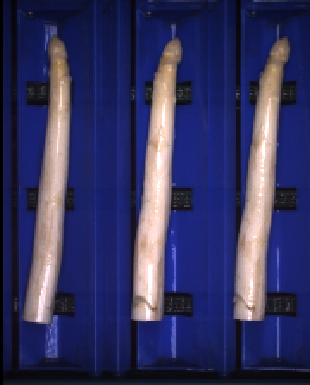
\includegraphics[width=0.9\linewidth]{Figures/chapter04/bent_falsenegative_03.png}
		\vspace{-5pt}
		\caption{False Negative}
	\end{subfigure}

	\begin{subfigure}{0.3\textwidth}
		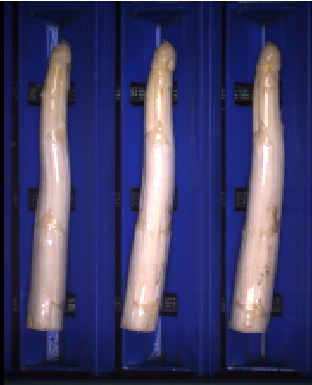
\includegraphics[width=0.9\linewidth]{Figures/chapter04/bent_falsepositive_01.png}
		\vspace{-5pt}
		\caption{False Positive}
	\end{subfigure}
	\begin{subfigure}{0.3\textwidth}
		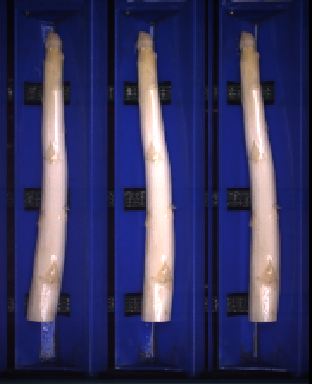
\includegraphics[width=0.9\linewidth]{Figures/chapter04/bent_falsepositive_02.png}
		\vspace{-5pt}
		\caption{False Positive}
	\end{subfigure}
	\begin{subfigure}{0.3\textwidth}
		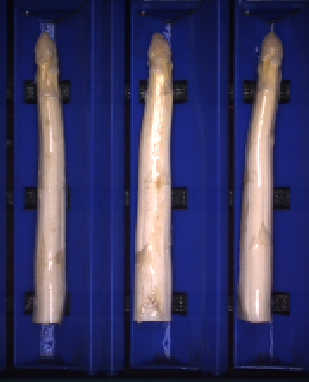
\includegraphics[width=0.9\linewidth]{Figures/chapter04/bent_falsepositive_03.png}
		\vspace{-5pt}
		\caption{False Positive}
	\end{subfigure}
	\vspace{-5pt}
    \caption[Single-Label CNN Example Images Feature Bent]{\textbf{Feature Bent}~~~Randomly chosen example images of false negatives and false positives of the feature bent after 3240 training steps. In all cases the presence of the feature bent is disputed. This becomes evident when comparing false negative and the false positive examples. The difference of both is not clearly evident (see the section~\nameref{subsec:Curvature} for a description of feature bent). It gives the impression that the human labelers did not sort with a strong threshold regarding the feature.}
    \label{fig:ExampleImagesBent}
\end{figure}

\bigskip
In~\autoref{tab:SingleLabelResults} the 13 features are listed on which the \acrshort{cnn} architecture was trained 13 times. It further shows the results for the sensitivity, specificity, validation accuracy, and balanced accuracy of each feature after a certain number of training steps, indicated in the last column of the table.

Sensitivity is a measure to assess the performance of the model in labelling positive samples correctly, while the specificity shows how correctly the model predicts negative samples. The validation accuracy is the accuracy of the validation set which is a representative subset of the entire data set. The balanced accuracy of a feature label is the mean of the sum of its sensitivity and specificity. It represents the accuracy of the feature label if positive and negative samples in the data set were evenly balanced.
Additionally, the performance of six models is calculated in a \acrshort{roc} curve in~\autoref{fig:SingleLabelROC}.\footnote{For an explanation of \acrshort{roc} curve, see \autoref{fig:FeatureEngineeringROC} in the previous section.} Models that determine features which indicate the thickness and length, as well as the feature not classifiable are excluded.
In the following discussion, it is referred to the best result of a model (depicted in brackets in~\autoref{tab:SingleLabelResults}) and not the last result.

The results reveal that for every feature, the sum of sensitivity and specificity exceeds 1.  This corresponds to a balanced accuracy over 50\%, which is better than chance level. For all features, the balanced accuracy is above 65\%. Best results are achieved for features that indicate the thickness of an asparagus. The feature very thick reaches the best results with 98\% sensitivity, 99\% specificity, and a balanced accuracy of 98.5\%. Besides features for thickness, the best prediction is observed for the feature fractured, which relies on the parameter length. It reaches a sensitivity of 88\%, a specificity of 99.8\%, and a balanced accuracy of 94\%.
On average, for the hand-labeled features a balanced accuracy above 72\% is reached. The feature rusty head performs worst with 52\% sensitivity, 81\% specificity, and 67\% balanced accuracy. In general, the specificity of all features is relatively high. Most features reach a specificity above 90\%, except for the features flower (83\%), rusty head (81\%), rusty body (80\%), and bent (73\%). For all features, the sensitivity is above 50\%. After visual inspection of test loss and training accuracy, none of the models showed any form of overfitting in their respective range of training steps.
Further, example images of wrong classification are shown for feature hollow in~\autoref{fig:ExampleImagesHollow} and for feature bent in~\autoref{fig:ExampleImagesBent}. Additional example images of false negative and false positive classification for the other features can be found in the appendix in~\autoref{subsec:AdditionalSingleLabelCNN}. For feature fractured, training and test loss as well as training and test accuracy are plotted as an exemplar in the appendix in~\autoref{fig:ExamplePlotsFractured}.\footnote{The models and their log files for accuracy and loss can be found at~\url{https://github.com/CogSciUOS/asparagus/tree/FinalProject/classification/supervised/single-label-CNN/asparanet} (as of 11/27/2020).}
 
\bigskip
The results indicate that the \acrshort{cnn} architecture is able to learn every feature. Features relying on the parameters of length and width achieve a good performance, with both validation accuracy and balanced accuracy above 90\%. The prediction of features like hollow or flower are expected to be more difficult. However, the balanced accuracy of both is above 75\%, with feature hollow even reaching a balanced accuracy of 88\%. This shows that the model predicts them relatively well. Features that depend on color (like rusty body, rusty head, and violet) do not reach equivalent results. It should be further tested whether an increase in model depth might lead to better results for features depending on color or for features depending on a more complex shape.
 
An inspection of false positive and false negative images at the end of the training process suggests that training performance might be influenced by mislabeled data to a certain extent.
The random images for feature hollow in \autoref{fig:ExampleImagesHollow} propose that the model might use the thickness of an asparagus as an indicator. Some of the samples look like hollow asparagus that could have been labeled incorrectly.
For the feature bent, the randomly selected examples in~\autoref{fig:ExampleImagesBent} might reveal a labeling bias by the human annotators. When the feature is only slightly present, it seems to become a random choice whether the sample was labeled as positive or negative by the human annotators. If true, this can make it difficult for the machine to perform above a certain level of accuracy. It might also be that the difference between the samples is not prominent enough to the model.
The results can also suggest that correct labeling might sometimes be difficult for the model because of an inconsistency in the labeling behavior of the human labelers (see \autoref{subsec:Reliability}).
 
On a general note, the architecture of the model is very flexible. It can be applied to many tasks (i.e.\ predicting different features) without much preprocessing of the image data beforehand. Further, the model is quite small, which makes it fast and robust for practical applications. However, instead of having the same architecture for all features, more precise adjustment of each model to its feature is needed.
 
\bigskip
In conclusion, the results of the single-label  \acrshort{cnn} seem promising. Due to a very long debugging phase, there was not enough time to further test and improve the performance of the model. In turn, this means there is still a lot of fine-tuning and possible improvement. A restriction poses the labeling bias of the manually labeled images.

\subsubsection{Multi-label classification}
\label{subsec:MultiLabel}

Building on the standard single-label classification we were further interested in how well a model, that predicts several feature labels at the same time, performs. A multi-label classification model hereby gets an image as the input and learns to predict the presence or absence of the feature labels.
For this model, we use a small  \acrshort{cnn} as described below and the features that we labeled by hand. Each of the six features (hollow, flower, rusty head, rusty body, bent and violet) is encoded by a binary output in the target vector, indicating whether the asparagus exhibits the feature in question or not.

\bigskip
Multi-label classification is a useful tool for classification problems in which several classes are assigned to a single input. In contrast to a multiclass classification, where the model is supposed to predict the most likely class for an input, the multi-label classification makes a prediction for each class separately, determining whether the class is present in the image or not. While the different classes are mutually-exclusive in the multiclass classification, they can be related in the multi-label classification. Further, there is no limit on how many classes can be depicted in one image. It is possible that all or none of the classes are present.

Multi-label classification tasks can be thought of as consisting of different sub tasks. Therefore, the problem can be transformed to multiple binary classification tasks. In this transformation, a new model for each feature is trained, which are then combined to give a single output. That means that all features are independent of one another because they are learned separately. This can be seen as one of the major drawbacks as in many cases features are related.
Therefore, we decided to not only use single-label classification as described in ~\autoref{subsec:SingleLabel} but to explore the possibilities of multi-label classification.

A second approach to transform a multi-label classification task is to interpret each possible combination of features as one class. Hereby, the problem is redefined as a multiclass classification task. For a classification problem with six features that means there are \(2^{6} = 64\) classes to be learned. The problems with this approach are, on the one hand, the exponentially increasing number of classes, and on the other hand, the sparsity of samples per class. In many cases, some of the classes are highly underrepresented or even empty. For that reason, we decided not to elaborate this approach further and implement a model for multi-label classification without transforming the task to a multiclass problem.

\bigskip
Inspiration for the model gave a blogpost~\citep{blogpostMulti} which aims to classify images of the MNIST fashion data set in the context of multi-label, rather than multiclass classification.
This model was chosen as inspiration for two main reasons. Firstly, it tackles a similar problem as ours and the number of classes is similar. Secondly, the model uses a data set of similar size. Despite the rather small data set in comparison to many other image classification problems, good results with an accuracy of 95 -- 96\% were reached~\citep{blogpostMulti}. This leads us to think, it might be a model with a good complexity for our problem too, as it is complex enough to model the underlying distribution, but not too complex for the medium-sized data set.

\begin{table}[!htb]
    \centering
    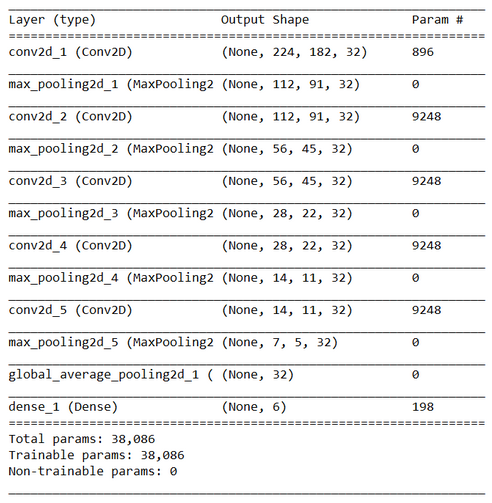
\includegraphics[scale=0.8]{Figures/chapter04/multilabel_structure.png}
    \decoRule
    \caption[Multi-Label Model Summary]{\textbf{Multi-Label Model Summary}~~~The summary of the multi-label classification model is shown. It describes which layers are implemented, how the output changes in each layer and how many parameters are trained in each layer and in total.}
    \label{tab:MultilabelStructure}
\end{table}

\bigskip
A classical \acrshort{cnn} was chosen for the multi-label classification task. It consists of five blocks of convolution layers with max pooling layers each followed by a global average pooling layer and a dense layer.

\begin{figure}[!htb]
    \centering
    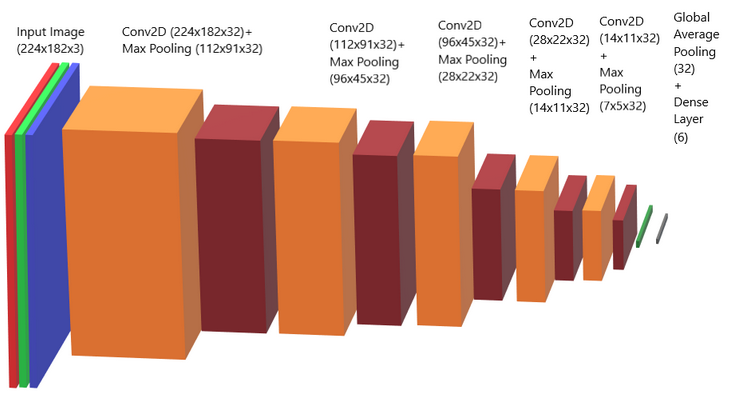
\includegraphics[width=0.95\textwidth]{Figures/chapter04/multilabel_net_structure.png}
    \decoRule
    \caption[Multi-Label Net Structure]{\textbf{Multi-Label Net Structure}~~~The depiction shows the network structure of the multi-label \acrshort{cnn}.}
    \label{tab:MultilabelNetStructure}
\end{figure}

In contrast to multiclass classification models, where usually a softmax activation function is used in the last layer together with a categorical cross-entropy loss, the multi-label classification model uses a sigmoid activation function and a binary cross-entropy loss.

As the input of the model, a concatenated image of the three perspectives of each spear is used in order to maximize the information the model gets. This yields input images where three asparagus spears are laying side by side. Further, the images are downscaled by a factor of six to facilitate training (see~\autoref{sec:AsparagusDataSet}).

As stated above, the output of the model is a vector of length six in which each position encodes one of the six hand-labeled features (hollow, flower, rusty head, rusty body, bent and violet). Each feature can either be present in the input or not, which leads to a 1 or 0 in the target vector, respectively.

Three loss functions are tested to improve the model's performance. The first two losses are in-built functions from keras, namely binary cross-entropy loss and hamming loss. The latter uses the fraction of the wrong labels to the total number of labels. Additionally, a custom loss function was implemented, that penalizes false negatives stronger than false positives. The motivation for this custom loss was the fact that the two labels 0 and 1 are highly unbalanced. As previously stated, there are noticeably more 0s than 1s in many classes. To be more precise, the model can reach an accuracy of 77\% by labeling all features as 0. By penalizing this error more, we intended to counteract the unbalanced data set. But at the end, the binary cross-entropy loss remains the one with the best results.

Further, it was tested whether regularization would improve the performance of the model on the validation data by preventing overfitting. For this, the model was trained by adding \(L_1\) or \(L_2\) regularization, respectively, to all five of the convolutional layers. Hereby, a kernel regularization was implemented with a value of 0.01.

\(L_1\) and \(L_2\) regularization can both be interpreted as constraints to the optimization that have to be considered when minimizing the loss term. The main difference between the two is that \(L_1\) regularization reduces the coefficient of irrelevant features to zero, which means they are removed completely. Hence, \(L_1\) regularization allows for sparse models and can be seen as a selection mechanism for features. The inputs to this model are images that consist of a large number of pixels, and additionally a large portion of those pixels are black, because the background was removed. Therefore, it appears to be a good idea to reduce the number of features taken into account in the early layers. \(L_2\) regularization, on the contrary, does not set coefficients to zero, but punishes large coefficients more than smaller ones. This way the error is better distributed over the whole vector.

\begin{figure}[!htb]
    \centering
    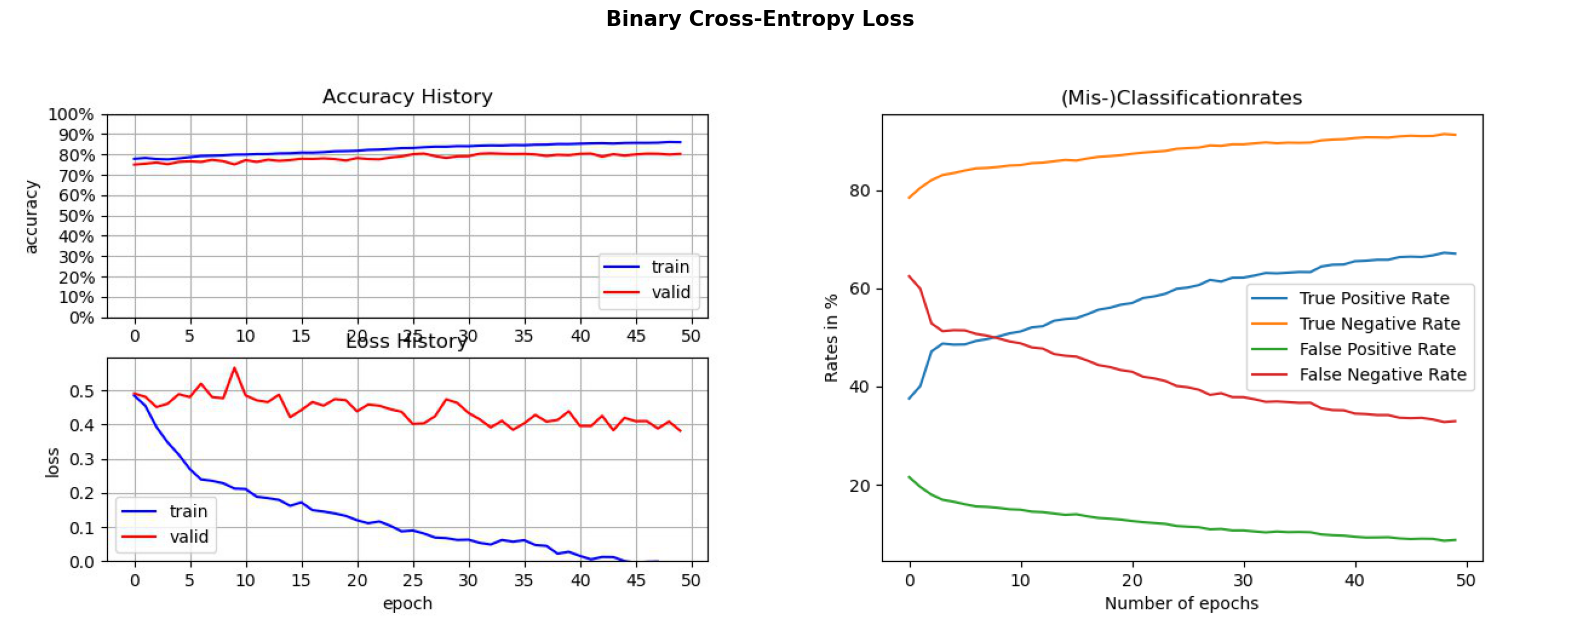
\includegraphics[scale=0.37]{Figures/chapter04/multilabel_crossentropy.png}
    \decoRule
    \caption[Multi-Label Binary Cross-Entropy Loss]{\textbf{Binary Cross-Entropy Loss}~~~These graphs show the evaluation of the training with binary cross-entropy loss. The model was trained over 50 epochs and the accuracy and loss was measured. Further, the false/true positive/negative rates were determined.}
    \label{fig:MultilabelCrossentropy}
\end{figure}

\begin{figure}[!htb]
    \centering
    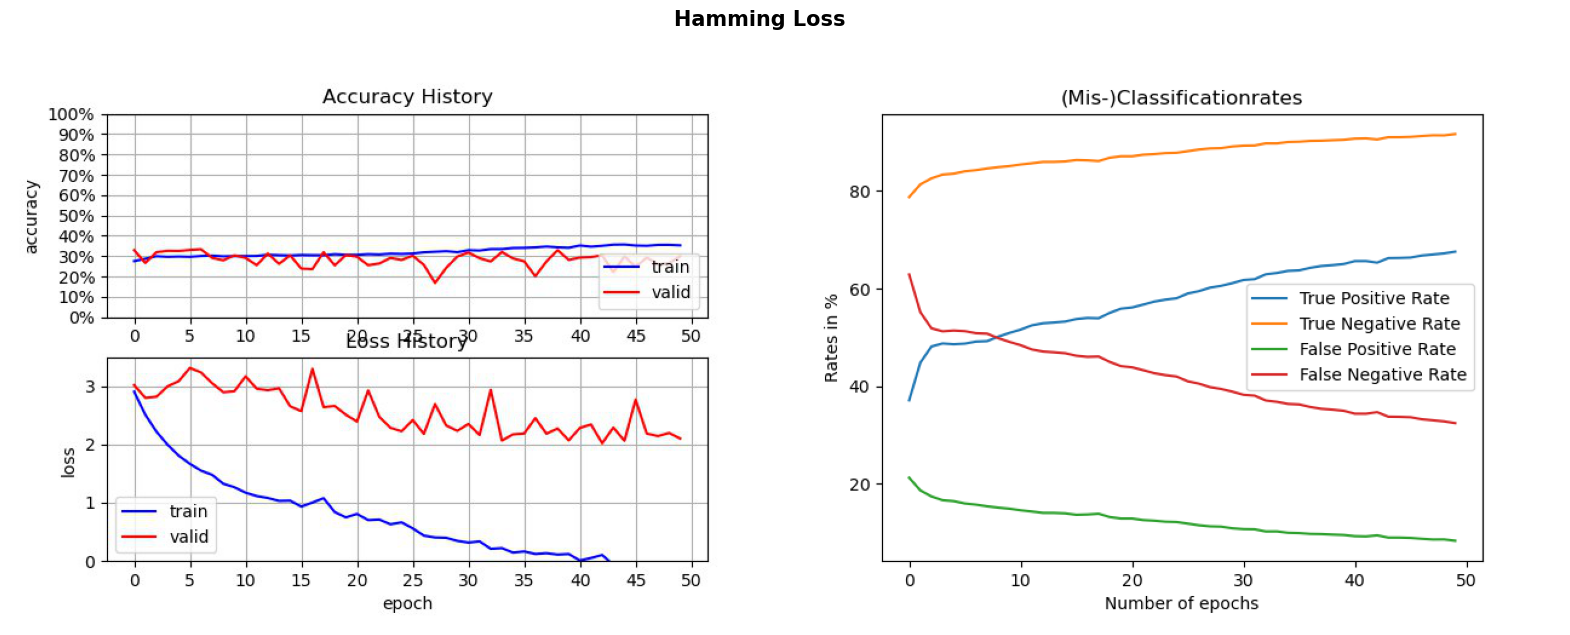
\includegraphics[scale=0.37]{Figures/chapter04/multilabel_hamming.png}
    \decoRule
    \caption[Multi-Label Hamming Loss]{\textbf{Hamming Loss}~~~These graphs show the evaluation of the training with hamming loss. The model was trained over 50 epochs and the accuracy and loss was measured. Further, the false/true positive/negative rates were determined.}
    \label{fig:MultilabelHammingLoss}
\end{figure}

\begin{figure}[!htb]
    \centering
    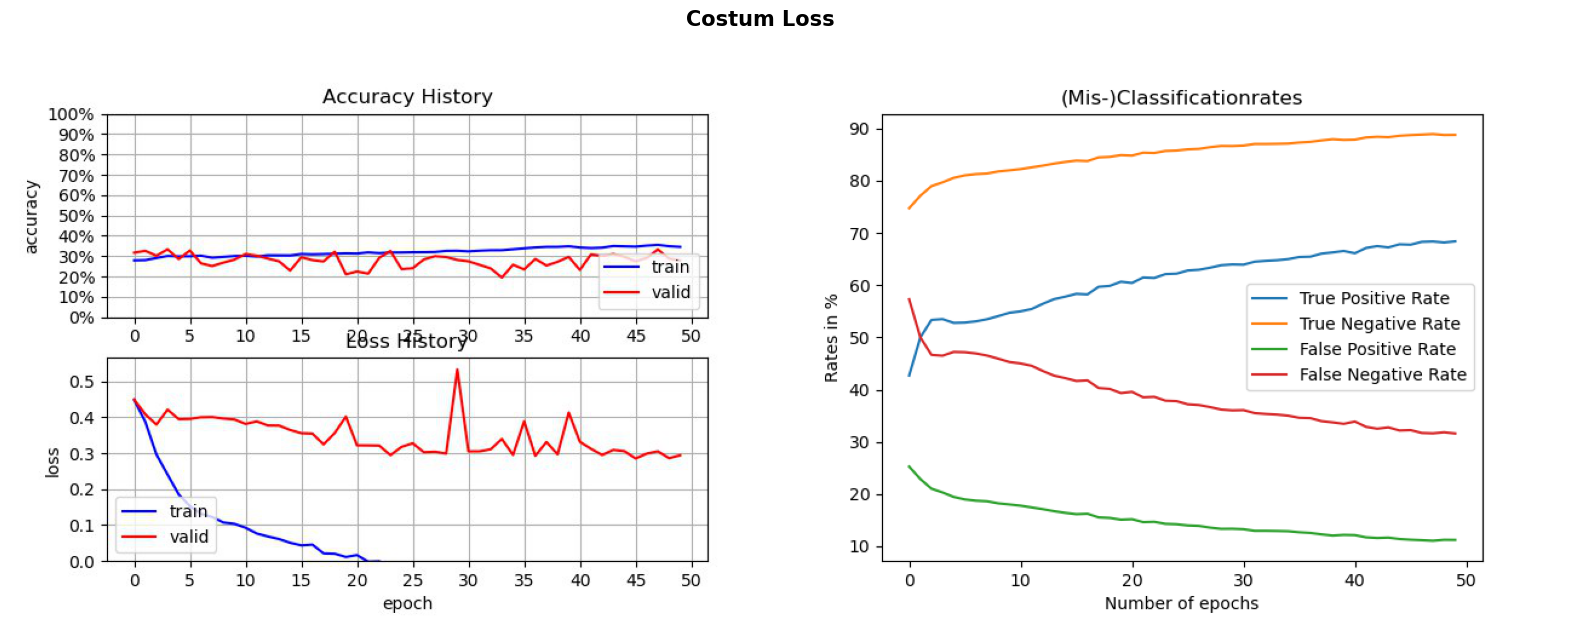
\includegraphics[scale=0.37]{Figures/chapter04/multilabel_costum.png}
    \decoRule
    \caption[Multi-Label Custom Loss]{\textbf{Custom Loss}~~~These graphs show the evaluation of the training with custom loss that punishes falsely classified ones more than falsely classified zeros. The model was trained over 50 epochs and the accuracy and loss was measured. Further, the false/true positive/negative rates were determined.}
    \label{fig:MultilabelCostumLoss}
\end{figure}

\begin{figure}[!htb]
    \centering
    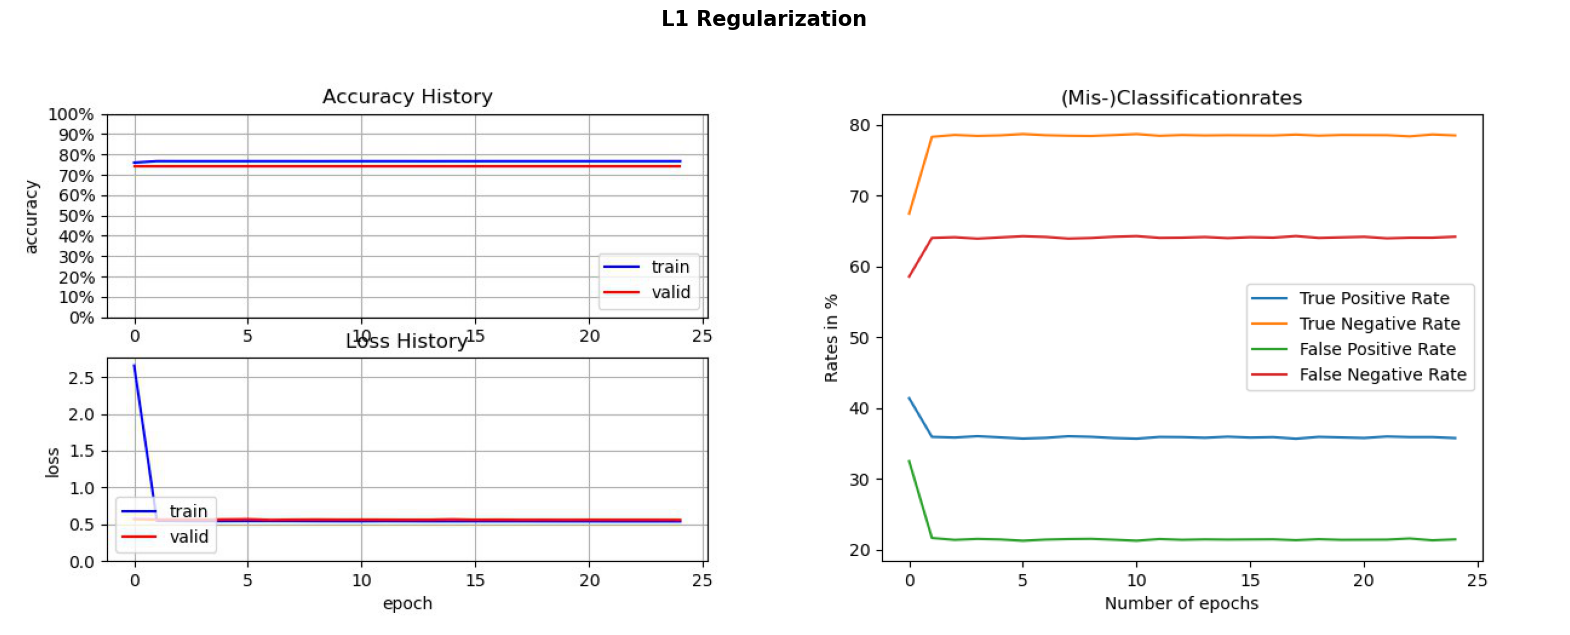
\includegraphics[scale=0.37]{Figures/chapter04/multilabel_L1.png}
    \decoRule
    \caption[Multi-Label \(L_1\) Regularization]{\textbf{\(L_1\) Regularization}~~~These graphs show the evaluation of the training with \(L_1\) regularization. As the loss function the binary cross-entropy loss was used. The model was trained over 25 epochs and the accuracy and loss was measured. Further, the false/true positive/negative rates were determined.}
    \label{fig:MultilabelL1Regularization}
\end{figure}

\begin{figure}[!htb]
    \centering
    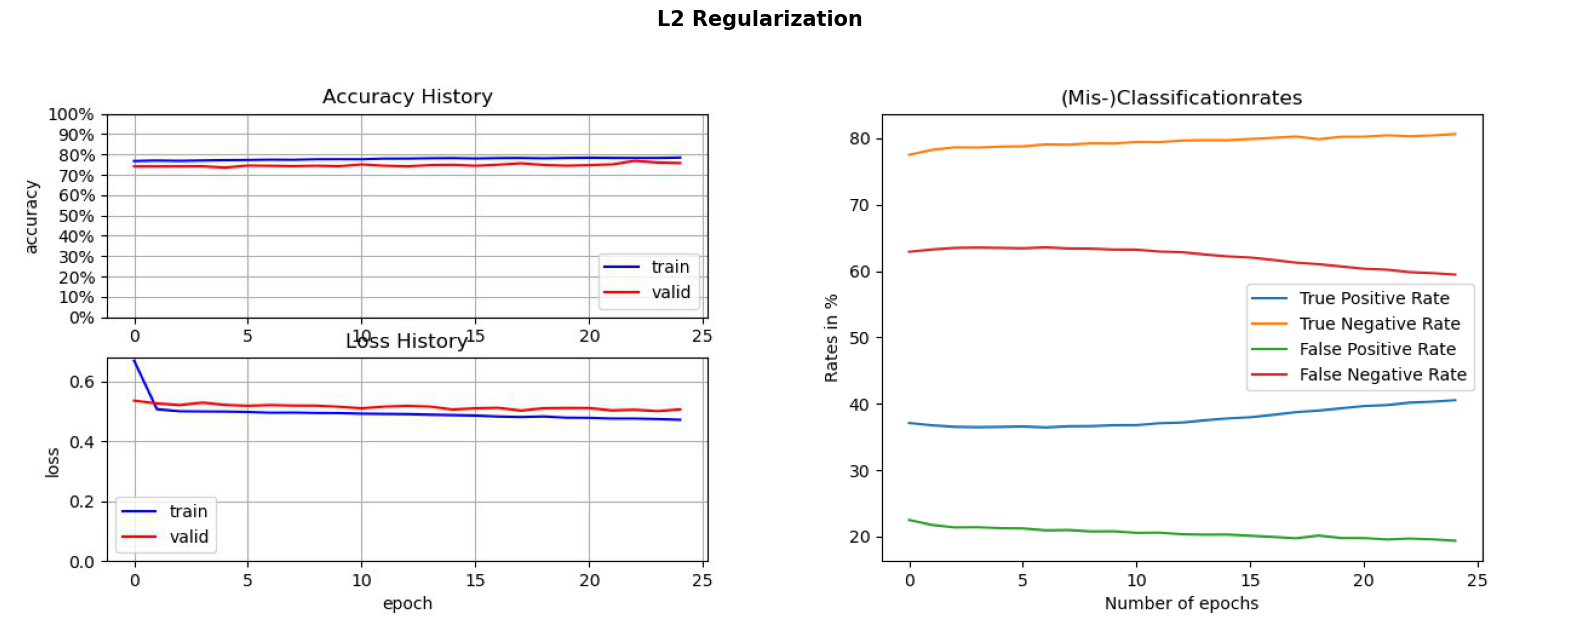
\includegraphics[scale=0.37]{Figures/chapter04/multilabel_L2.png}
    \decoRule
    \caption[Multi-Label \(L_2\) Regularization]{\textbf{\(L_2\) Regularization}~~~These graphs show the evaluation of the training with \(L_2\) regularization. As the loss function the binary cross-entropy loss was used. The model was trained over 25 epochs and the accuracy and loss was measured. Further, the false/true positive/negative rates were determined.}
    \label{fig:MultilabelL2Regularization}
\end{figure}

As shown in \autoref{fig:MultilabelCrossentropy}, \autoref{fig:MultilabelHammingLoss} and \autoref{fig:MultilabelCostumLoss}, all the different approaches explained above show a similar behavior in accuracy and loss values. The training and validation accuracy increase slowly but steadily with the training accuracy always being a little higher than the validation accuracy. The training loss decreases rapidly, while the validation loss only decreases very little and shows random fluctuations. This can be an indicator for overfitting. Usually, \(L_1\) and \(L_2\) regularization are used to prevent overfitting, but in our case it did not improve the results, as shown in \autoref{fig:MultilabelL1Regularization} and \autoref{fig:MultilabelL2Regularization}.

When looking at the sensitivity and specificity, it becomes apparent that both increase during the training process, while the false negative and false positive rates decrease with the same slope. The false positive and false negative rates are mirror images to the true positive and true negative rates with the mirroring axis at the 50\% mark. It can be observed that the rates change rapidly in the first two to four epochs, after which the change progresses slowly in the same direction with no greater disturbances. The model trained with the \(L_2\) loss is an exception as it does not show these large changes in either of the rates.

\bigskip
When comparing the three different loss functions, it is noticeable that the binary cross-entropy loss has significantly larger accuracy values than the hamming loss and the custom loss. The values of the binary cross-entropy loss start at 75\% and reach the highest accuracy with 87\%, while they start at around 30\% and only reach values between 45\% to 47\% for the other two loss functions. The behavior of the curves and the (mis-)classification rates, however, are very similar in all three approaches. The specificities start off very high with values around 78.46\% for the binary cross-entropy loss, 78.73\% for the hamming loss and 74.74\% for the custom loss, and increase further during the training. The highest values are reached with the binary cross-entropy loss (91.41\%), closely followed by the hamming loss (91.37\%) and the custom loss (88.75\%). The sensitivity values start off lower, at around 37\% to 42\%, and increase rapidly in the first few epochs, after which the rates proceed to increase but with a narrower slope. They reach values of up to 67.27\% with the binary cross-entropy loss, 68.17\% with the hamming loss and 68.17\% with the custom loss. As stated above, the false negative and false positive rates show the same slope but in the opposite direction.

The accuracy values of the models that are trained with \(L_1\) or \(L_2\) regularization, respectively, do not change over the epochs. The same holds for the validation loss. The training loss decreases in the first few epochs and remains stable thereafter.
While the (mis-)classification rates of the model trained with \(L_1\) regularization behave similarly to the ones trained with no regularization, the rates of the model trained with \(L_2\) regularization show a smaller increase and lack the fast change in the first epochs.

The slopes of all curves indicate that the model is learning, because they are increasing in the case of the accuracy, sensitivity and specificity and decreasing in the case of the loss, false positive and false negative rates until the end of training. Hence, one might think that a longer training period will lead to better results. However, the training loss decreases very rapidly while the validation loss does not. This suggests overfitting of the model, a problem which gets worse when increasing the training steps. Therefore, a longer training period most likely will not increase performance unless overfitting is prevented. As shown in the result section, neither \(L_1\) nor \(L_2\) regularization alone were able to prevent overfitting.

Another common practice that can be tested in the future is the drop-out, in which a certain amount of nodes are left out in different backpropagation steps. This way the model learns to not rely on a small number of nodes but distribute the information between all nodes available. Hence, the coefficients remain smaller. Another method to prevent overfitting is to reduce the model's complexity. A model with fewer parameters to train, is less prone to overfitting. A fitting degree of complexity should be found to model the data sufficiently good without losing the possibility of generalization.

Accuracy alone might not be a good indicator to evaluate a multi-label model~\citep{gibaja2015}. As it highly depends on the loss function, it may have misleading results. This can be seen in the comparison between the three different loss functions. Although the sensitivity and specificity show similar values, the accuracy values suggest that the binary cross-entropy loss outperforms the other two loss functions by far. The accuracy of the model trained with the binary cross-entropy loss has an accuracy more than twice as high. But when looking at the slope of the curve, it appears that the model with the binary cross-entropy loss does not perform better than the other two models. All three have an increase of accuracy of roughly 10\% and a similar sensitivity and specificity. This indicates that the slope of the accuracy function can be considered to evaluate the training process of the model, but the real values should be interpreted with caution.

One thing that comes to attention when looking at the (mis-)classification rates is that the sensitivities are a lot lower than the specificities. A reason for that might be that the positive values are more difficult to learn because they are only sparsely present. The model might have learned that, if the allocation to an output class is not clear, a 0 is the more likely guess.

The \(L_1\) and \(L_2\) regularization both seem to prevent the model from learning all together instead of only preventing overfitting. A reason for that might be that the regularization factor is too high. More experiments should be conducted with varying values to test this hypothesis.

\bigskip
In summary, the model improves its sensitivity and specificity, but it seems like it does so by overfitting the training data. Therefore, the next step should be to prevent the model from overfitting. Afterwards, it should be tested whether additional changes can improve the performance of the model further.


\subsubsection{A dedicated network for head-related features}
\label{subsec:HeadNetwork}

Some features relate to the asparagus heads only. Hence, it was assumed that classification is easiest when training a \acrshort{cnn} on depictions of the respective region of the asparagus. Therefore, a data set that consists only of images of the head area is used. Images of all three perspectives are appended horizontally such that each sample contains the information from all available viewpoints. This is especially important as rust affected spots are sometimes only visible from certain angles. \autoref{fig:HeadExample} shows one sample of a rust affected asparagus head.

\begin{figure}[!htb]
	\centering
	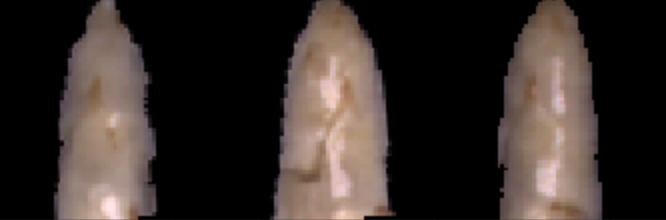
\includegraphics[scale=0.4]{Figures/chapter04/head_example.png}
	\decoRule
	\caption[Head Features CNN Training Sample]{\textbf{Training Sample}~~~The depiction shows a sample for the preprocessed and vertically aligned asparagus head. Mind that images from all perspectives were stacked horizontally and used as a single input for the \acrshort{cnn}.}
	\label{fig:HeadExample}
\end{figure}

\begin{figure}[!htb]
	\centering
	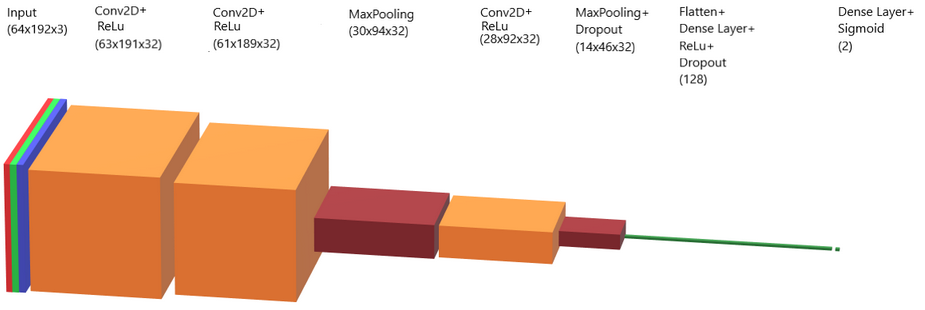
\includegraphics[width=0.95\textwidth]{Figures/chapter04/head_net_structure.png}
	\decoRule
	\caption[Head Features Net Structure]{\textbf{Head Features Net Structure}~~~The depiction shows the network structure of the \acrshort{cnn} specifically aimed at head features.}
	\label{fig:HeadNetStructure}
\end{figure}

\bigskip
A simple feedforward \acrshort{cnn} was trained on the images.\footnote{~See \url{https://github.com/CogSciUOS/asparagus/tree/FinalProject/classification/supervised/dedicated\_head\_network} (as of 11/27/2020)} The features flower and rusty head are chosen as target categories. Hence, the  model is an example for multi-label classification. The network comprises the input layer, three convolutional layers with kernel size two, a fully connected layer with 128 neurons as well as the output layer. For the final layer, the sigmoid activation function is applied while the hidden layers have ReLU activations. A dropout layer was added to avoid overfitting. The network was trained using \acrfull{mse} as an error function. The development of loss in the learning curve indicates convergence after 40 epochs (see \autoref{fig:HeadCurve}).

\begin{figure}[!htb]
	\centering
	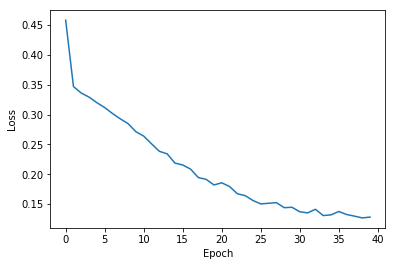
\includegraphics[scale=1.8]{Figures/chapter04/head_curve.png}
	\decoRule
	\caption[Head Features CNN Learning Curve]{\textbf{Learning Curve for the Head Features CNN}~~~The depiction shows the loss per training episode for the \acrshort{cnn} trained on asparagus heads.}
	\label{fig:HeadCurve}
\end{figure}	

\begin{figure}[!t]
	\centering
	\vspace{2cm}
	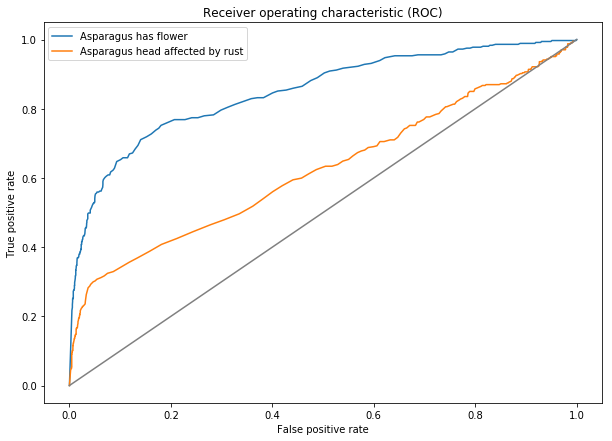
\includegraphics[scale=1.55]{Figures/chapter04/head_roc.png}
	\decoRule
	\caption[Head Features CNN ROC Curve]{\textbf{ROC for the Head Features CNN}~~~The depiction shows the \acrfull{roc} for the predictions of the \acrshort{cnn} trained on asparagus heads. It allows us to compare the performance. A larger area under the \acrshort{roc} curve indicates better performance while a curve close to the diagonal line indicates poor results.}
	\label{fig:HeadROC}
\end{figure}

\bigskip
The results for both features show to be highly specific. In contrast, the sensitivity is rather low. Only 55\% of the asparagus spears labeled as flower are identified as such whereas the true positive rate is only 19\% for rusty head. Given the low labeling agreement for these criteria (see \autoref{subsec:Reliability}), these mediocre results are not surprising.

The \acrshort{roc} curve indicates how the classifiers respond to the introduction of a bias and shows the overall prediction quality. In \autoref{fig:HeadROC} the area under the curve is small for the feature rusty head. Beside incongruencies in the labels, this is possibly due to the choice of the size of the head region. It might be the case that brown spots in regions other than the cropped part were considered as an indicator for a rusty head when attributing labels. Improvements by increasing the cropped head region appear to be possible.

\begin{table}[!htb]
	\centering
	\resizebox{\columnwidth}{!}{%
	\begin{tabular}{lrrrrrr}
		{} &  False positive &  False negative &  True positive &  True negative &  Sensitivity &  Specificity \\
		\noalign{\smallskip}
		\hline
		\noalign{\smallskip}	
		flower     &            0.04 &            0.06 &           0.08 &           0.82 &         0.55 &         0.95 \\
		rusty head &            0.02 &            0.13 &           0.03 &           0.83 &         0.19 &         0.98 \\
		\noalign{\smallskip}
		\hline
	\end{tabular}%
	}
	\caption[Head Features CNN Performance]{\textbf{Performance of Head Features CNN}~~~Performance of the \acrshort{cnn} trained on asparagus heads.}
	\label{tab:performance_measures_head_based}
\end{table}


\subsubsection{From hand-labeled features to class labels}
\label{subsec:FeaturesToLabels}

Approximately 200 asparagus spears per class label serve as ground truth mappings between input images and output class labels. We manually annotated the images with features (see \autoref{sec:ManualLabeling}). This allows us to divide the classification process into two steps: In the first step we predict feature values from images and in a second step we predict class labels from those feature values.

\begin{figure}[!htb]
    \centering
    \includegraphics[width=0.60\textwidth]{Figures/chapter04/ftl_pipeline.png}
    \decoRule
    \caption[Feature to Class Label Pipeline]{\textbf{Feature to Class Label Pipeline}~~~The figure shows the flow of data and visualizations of our end to end solution app. We developed an app into which the user can load the asparagus images and the corresponding annotations. The app then visualizes the class label distribution. The user can choose a model to predict the features of the asparagus pieces and inspect predictions for individually selected samples. Next, the user chooses a model that predicts class labels based on features of the asparagus. The app then presents a classification report, a confusion matrix and the possibility to inspect individual samples to visualize the prediction performance.}
    \label{fig:FeatureEngineeringNetStructure}
\end{figure}

\begin{figure}[!htb]
    \centering
    \includegraphics[scale=0.4]{Figures/chapter04/ftl_streamlit_app.png}
    \decoRule
    \caption[Screenshot of the Streamlit App]{\textbf{Screenshot of Streamlit App}~~~Screenshot of the streamlit app showing the three images of one asparagus spear with the corresponding labeled features.}
   \label{fig:FeaturetoLabelStreamlitApp}
\end{figure}   

\begin{figure}[!htb]
    \centering
    \includegraphics[scale=0.55]{Figures/chapter04/ftl_visualization.png}
    \decoRule
    \caption[Distribution of Class Labels]{\textbf{Distribution of Class Labels}~~~Absolute number of the asparagus spears for which a ground truth class label is available.}
    \label{fig:FeatureToLabelVisualization}
\end{figure}

\begin{figure}[!htb]
    \centering
    \includegraphics[scale=0.4]{Figures/chapter04/ftl_confusion_recall_random_forest.png}
    \decoRule
    \caption[Random Forest Classifier Confusion Matrices]{\textbf{Random Forest Classifier Confusion Matrices}~~~Confusion matrices showing the absolute and relative number of true positives of the random forest model.}
    \label{fig:FeatureToLabelRandomForest}
\end{figure}

%\begin{table}[!ht]
%    \centering
%    \includegraphics[scale=0.5]{Figures/chapter04/ftl_classification_report.png}
%    \decoRule
%    \caption[Classification Report of the Random Forest Classifier]{\textbf{Classification Report of the Random Forest Classifier}~~~The classification report shows key metrics for the trained random forest classifier.}
%    \label{tab:FeatureToLabelReport}
%\end{table}

\bigskip
This chapter deals with the second step: Using supervised learning to predict 13 class labels, referring to the classes at the asparagus farm Gut Holsterfeld, based on the manually labeled features. We built a unified interface to load different models, train them and analyze their predictions. It provides compatibility for scikit-learn as well as for keras models. To explore the data and visualize the predicted results, we built a streamlit app.\footnote{inside code/pipeline in the GitHub repository} This has the advantage that the user can easily load and train a model, select an asparagus spear, and see the corresponding images as well as the predicted class label (see \autoref{fig:FeaturetoLabelStreamlitApp}).

The user can also inspect the distribution of the selected data (\autoref{fig:FeatureToLabelVisualization}) and the absolute and relative number of correctly and incorrectly classified asparagus spears in a confusion matrix (\autoref{fig:FeatureToLabelRandomForest}).

The precision and recall are measures on how \enquote{useful and complete} the results are \citep{wiki:precisionrecall}. Precision is the ratio between true positives and the set of all true and false positives. Recall is the ratio between the true positives and the set of all true positives and false negatives. The confusion matrix (\autoref{fig:FeatureToLabelRandomForest}) gives us insight about which kind of errors the models make. We can observe that classes such as I~A~Anna, Dicke, Hohle, Rost, Köpfe, and Suppe can be recalled well (relative recall $\geq$ 0.8), while other classes, such as II~A and II~B have much lower recall ratings (relative recall $\leq$ 0.6). That means that II~A and II~B are the most commonly mislabeled classes (cf.~\autoref{tab:FeatureToLabelReport}).

\begin{table}[!h]
    \centering
    \resizebox{.65\textwidth}{!}{%
    \begin{tabular}{ l r r r r r r }
        {} & precision & recall & f1-score & support \\
        \noalign{\smallskip}
    		\hline
    		\noalign{\smallskip}
I~A Anna      & 0.7360      & 0.8936   & 0.8077     & 47      \\
\smallskip
I~A Bona      & 0.7000      & 0.7241    & 0.7119     & 58      \\
\smallskip
I~A Clara     & 0.7368      & 0.7368   & 0.7368      & 57      \\
\smallskip
I~A Krumme    & 0.6667      & 0.6400   & 0.6531     & 50      \\
\smallskip
I~A Violett    & 0.6481      & 0.7609   & 0.7000     & 46      \\
\smallskip
II~A           & 0.6842      & 0.4643   & 0.5532     & 56      \\
\smallskip
II~B           & 0.7179       & 0.5600   & 0.6292     & 50      \\
\smallskip
Blume        & 0.6939      & 0.7556   & 0.7234     & 45      \\
\smallskip
Dicke        & 0.7000      & 0.7955   & 0.7447     & 44      \\
\smallskip
Hohle        & 0.9459      & 0.8974    & 0.9211     & 39      \\
\smallskip
Koepfe       & 1           & 1      & 1        & 38      \\
\smallskip
Rost         & 0.8305      & 0.8909   & 0.8596     & 55      \\
\smallskip
Suppe        & 0.9444      & 0.9189   & 0.9315     & 37      \\
\smallskip
accuracy     & 0.7588      & 0.7588   & 0.7588     & 0.7588    \\
\smallskip
avg          & 0.7696      & 0.7722   & 0.7671     & 622     \\
\smallskip
weighted avg & 0.7591      & 0.7588   & 0.7549     & 622    \\
\noalign{\smallskip}
\hline
    \end{tabular}%
    }
    \caption[Classification Report of the Random Forest Classifier]{\textbf{Classification Report of the Random Forest Classifier}~~The classification report shows key metrics for the trained random forest classifier.}
    \label{tab:FeatureToLabelReport}
\end{table}

\bigskip
Two exemplary models were implemented and tested to predict the classes from the features. The first one is a random forest~\citep{breiman2001random} with 100 trees.

The second model to predict classes from features is an \acrshort{mlp} with six fully connected layers. It is only implemented to show how to integrate other models, but achieves a similar score as the random forest classifier when trained for 500 epochs (score of 0.76). However, it takes longer to train than the random forest classifier.

The score of 0.76 on the validation set is the accuracy of the random forest classifier, that means that 76\% of the data is predicted correctly –- random guessing would yield an accuracy of 0.08 for uniformly distributed classes.

\bigskip
Although the results point into the right direction, it would be interesting to see how the selection of features and the agreement on the values of the manually labeled features influence the performance of the described classifiers. Further work is required to implement the decision process described by the local farmer (see \autoref{sec:BackgroundSortingAsparagus}). One could test if the decision tree based on expert knowledge in \autoref{fig:LabelTree}) can outperform the random forest trained on the training samples.


\subsection{Unsupervised learning}
\label{sec:UnsupervisedLearning}

Unsupervised learning is a class of machine learning techniques that deals with unlabeled data. More specifically, they work without a known goal, a reward system or prior training, and are usually used to find structure within data. Dimension reduction algorithms and clustering algorithms have been identified as the two main classes of unsupervised machine learning algorithms which are used in image categorization~\citep{olaode2014}. 

\bigskip
Multivariate data sets are generally high dimensional. However, it is common that some parts of that variable space are more filled with data points than others. A large part of the high dimensional variable space is not used. In order to recognize a structure or pattern in the data, it is necessary to reduce the number of dimensions. For this, both linear and non-linear approaches can be applied. Linear unsupervised learning methods for which also descriptive statistics can be acquired are e.g.\ \acrfull{pca}, non-negative matrix factorization, and Independent Component Analysis~\citep{olaode2014}. Some examples for non-linear approaches are Kernel \acrshort{pca}~\citep{olivier2006semi}, Isometric Feature Mapping,  Local Linear Embedding, and Local Multi-Dimensional Scaling. We employed the linear dimension reduction algorithm \acrshort{pca} as well as autoencoders for nonlinear dimension reduction.


\subsubsection{Principal Component Analysis}
\label{subsec:PCA}

\acrlong{pca} was performed, because it is one of the standard unsupervised machine learning methods. Moreover, it is a linear, non-parametric method and a widespread application to extract relevant information from high dimensional data sets. The goal is to reduce the complexity of the data by only a minor loss of information~\citep{shlens2014}. Besides being a dimension reduction algorithm, \acrshort{pca} can also be useful to visualize or compress the data, filter noise, or extract features.

\bigskip
Our initial aim was to reduce the dimension of our data set for further models. As \acrshort{pca} was applied at the beginning of the data inspection, we also had the aim to visualize our data in a three-dimensional space, in order to get a better understanding of the data distribution. The images that comprise our original data set have a high quality, and instead of only reducing the pixel size, we aimed to reduce the information contained in named depictions. It was achieved by analyzing the principal components in a first step, followed by projecting all relevant images into the lower dimensional space. This information could serve as the input to supervised machine learning algorithms or as a simple lookup scheme to retrieve the label of the example with the most similar low dimensional representation.

\bigskip
\acrshort{pca} relies on linear algebra. A general assumption, especially with respect to images, is that large variances are accompanied by important structure \citep{shlens2014}. The covariance matrix of the data reveals information about the overall structure and orientation of the data points in the multivariate space. The axis with the largest variance is set as the first principal component. An additional assumption is that the principal components are orthogonal to each other. Therefore, the second principal component is the highest variability of all directions which are orthogonal to the first one \citep{bohling2006}. The covariance between each pair of principal components is zero, as they are uncorrelated. It generally holds that the higher the eigenvalues are, the more useful they are for the analysis. As eigenvalues specify the variance of the data, higher eigenvalues indicate more relevant features \citep{shlens2014}.

The result of a \acrshort{pca} is a representation of the data in a new, smaller coordinate system, which depends on the axes of the largest variance. The dimensionality of this lower coordinate system should depend on the magnitude of the eigenvalues. When plotting the data along the axes of the principal components, it is often easier to understand and interpret the data, than in the original variable space.

It is widely agreed upon that \acrshort{pca} can be a good method to apply dimension reduction on images~\citep{turk1991face,lata2009}.
However, there are several different ways on how to do so. First of all, we performed the \acrshort{pca} on black and white images. When working on black and white images, only one data point per pixel is given. Therefore, performing a \acrshort{pca} is less computationally expensive, and finding structure is easier. However, as we need to be able to recognize violet as well as rust, and therefore be able to differentiate between color nuances, it was decided to work on colored images.

\bigskip
There are various possibilities on what to apply the \acrshort{pca}. First, it can be performed on images of different classes at the same time – similar to capturing several images of several people in one database, on which one \acrshort{pca} is performed. In our case this would mean that a \acrshort{pca} is applied to a data set of several input images of all 13 class labels. The second way would be to perform a \acrshort{pca} separately on each class. This way, an \enquote{Eigenasparagus} in each class would be calculated, and distances between the Eigenasparagus of different classes could be measured. Thirdly, \acrshort{pca} can be employed feature-wise. In this case, the data set would consist of a collection of images with a certain feature present in contrast to a collection of the same size with the feature absent.

\bigskip
After trying several different approaches, we decided to perform our final \acrshort{pca} on sliced RGB images with background. The images were labeled for their features with the hand-label app, as this yielded the best results. An amount of 400 pictures per feature was used to perform a binary \acrshort{pca} for each feature (either the feature is absent or present).

For each feature a matrix is created, storing 200 pictures with the present feature and 200 pictures without the feature. E.g.\, m\textunderscore hollow is the matrix created for the feature hollow (shape = 400, img\textunderscore shape[0] $\times$ img\textunderscore shape[1] $\times$ img\textunderscore shape[2]). The first 200 entries in the matrix are pictures of hollow asparagus. The last 200 pictures show asparagus, which is not hollow. These matrices were calculated for the features hollow, flower, rusty head, rusty body, bent, violet, length, and width. The data points of those 400 images in 2D space can be seen in~\autoref{fig:PCAscatter}.

\begin{figure}[!htb]
	\centering
	\includegraphics[width=0.98\textwidth]{Figures/chapter04/pca_process.png}
	\decoRule
	\caption[PCA Process]{\textbf{PCA Process}~~~Before the \acrshort{pca} can be conducted, 200 images per feature are identified by the \texttt{get\textunderscore feature\textunderscore ids} function. Then, a matrix for each feature is calculated. The \acrshort{pca} is conducted feature-wise. Thereafter, an Eigenspace for each feature is calculated. To evaluate the performance of the \acrshort{pca}, a verification process was performed. Therefore, new feature-labeled asparagus pictures are taken as input and by the help of all Eigenspaces, they evaluate if the feature is present \enquote{1} or absent \enquote{0}. The result is compared to the label in order to evaluate the performance of the Eigenspace. To improve the algorithm, a pipeline of calculations can be implemented such that a feature vector is calculated. This feature-vector gives a class prediction. This is compared to the known label of the image.}
	\label{fig:PCAprocess}
\end{figure}

\begin{figure}[!h]
	\centering
	\begin{subfigure}{0.7\textwidth}
		\includegraphics[width=0.9\linewidth]{Figures/chapter04/pca_length_graph.png} 
		\caption{This plot shows the magnitude of the first ten eigenvalues for the feature length.}
	\end{subfigure}
	\vspace{20pt}
	
	\begin{subfigure}{0.9\textwidth}
		\includegraphics[width=0.9\linewidth]{Figures/chapter04/pca_length.png}
		\caption{These images show the first ten Eigenasparagus of the feature length.}
	\end{subfigure}
	\caption[First Ten Eigenvalues and Eigenasparagus of Feature Length]{\textbf{Eigenvalues and Eigenasparagus of Feature Length}~~~(A) This plots shows the magnitude of the first ten eigenvalues for the feature length. (B) These images show the first ten Eigenasparagus of the feature length.}
    \label{fig:PCAlength}
\end{figure}

%\begin{figure}
%    \centering
%    \subfloat[]{\includegraphics[width=6.5cm]{Figures/chapter04/pca_length_graph}}
%    \qquad
%    \subfloat[]{\includegraphics[width=6.5cm]{Figures/chapter04/pca_length}}
%    \caption[First ten Eigenvalues and "Eigenasparagus" of Feature Length]{\textbf{Eigenvalues and "Eigenasparagus" of Feature Length}~~~(A) This plots shows the magnitude of the first ten eigenvalues for the feature length. (B) These images show the first ten “Eigenasparagus” of the feature length.}
%    \label{fig:PCAlength}
%\end{figure}

\begin{figure}[!h]
	\centering
	\begin{subfigure}{0.7\textwidth}
		\includegraphics[width=0.9\linewidth]{Figures/chapter04/pca_hollow_graph.png} 
		\caption{This plot shows the magnitude of the first ten eigenvalues for the feature hollow.}
	\end{subfigure}
	\vspace{20pt}
	
	\begin{subfigure}{0.9\textwidth}
		\includegraphics[width=0.9\linewidth]{Figures/chapter04/pca_hollow.png}
		\caption{These images show the first ten Eigenasparagus of the feature hollow.}
	\end{subfigure}
    \caption[First Ten Eigenvalues and Eigenasparagus of Feature Hollow]{\textbf{Eigenvalues and Eigenasparagus of Feature Hollow}}
    \label{fig:PCAhollow}
\end{figure}

%\begin{figure}
%    \centering
%    \subfloat[]{\includegraphics[width=6.5cm]{Figures/chapter04/pca_hollow_graph}}
%    \qquad
%    \subfloat[]{\includegraphics[width=6.5cm]{Figures/chapter04/pca_hollow}}
%    \caption[First ten Eigenvalues and "Eigenasparagus" of Feature Hollow]{\textbf{Eigenvalues and "Eigenasparagus" of feature hollow}~~~(A) This plots shows the magnitude of the first ten eigenvalues for the Feature Hollow. (B) These images show the first ten “Eigenasparagus” of the feature hollow.}
%    \label{fig:PCAhollow}
%\end{figure}

\begin{figure}[!h]
	\centering
	\begin{subfigure}{0.7\textwidth}
		\includegraphics[width=0.9\linewidth]{Figures/chapter04/pca_bent_graph.png} 
		\caption{This plot shows the magnitude of the first ten eigenvalues for the feature bent.}
	\end{subfigure}
	\vspace{20pt}
	
	\begin{subfigure}{0.9\textwidth}
		\includegraphics[width=0.9\linewidth]{Figures/chapter04/pca_bent.png}
		\caption{These images show the first ten Eigenasparagus of the feature bent.}
	\end{subfigure}
    \caption[First Ten Eigenvalues and Eigenasparagus of Feature Bent]{\textbf{Eigenvalues and Eigenasparagus of Feature Bent}}
    \label{fig:PCAbent}
\end{figure}

%\begin{figure}
%    \centering
%    \subfloat[]{\includegraphics[width=6.5cm]{Figures/chapter04/pca_bent_graph}}
%    \qquad
%    \subfloat[]{\includegraphics[width=6.5cm]{Figures/chapter04/pca_bent}}
%    \caption[First ten Eigenvalues and "Eigenasparagus" of Feature Bent]{\textbf{Eigenvalues and "Eigenasparagus" of Feature Bent}~~~(A) This plots shows the magnitude of the first ten eigenvalues for the feature bent. (B) These images show the first ten “Eigenasparagus” of the feature bent.}
%    \label{fig:PCAbent}
%\end{figure}

\begin{figure}[!h]
	\centering
	\begin{subfigure}{0.7\textwidth}
		\includegraphics[width=0.9\linewidth]{Figures/chapter04/pca_violet_graph.png} 
		\caption{This plot shows the magnitude of the first ten eigenvalues for the feature violet.}
	\end{subfigure}
	\vspace{20pt}
	
	\begin{subfigure}{0.9\textwidth}
		\includegraphics[width=0.9\linewidth]{Figures/chapter04/pca_violet.png}
		\caption{These images show the first ten Eigenasparagus of the feature violet.}
	\end{subfigure}
    \caption[First Ten Eigenvalues and Eigenasparagus of Feature Violet]{\textbf{Eigenvalues and Eigenasparagus of Feature Violet}}
    \label{fig:PCAviolet}
\end{figure}

%\begin{figure}
%    \centering
%    \subfloat[]{\includegraphics[width=6.5cm]{Figures/chapter04/pca_violet_graph}}
%    \qquad
%    \subfloat[]{\includegraphics[width=6.5cm]{Figures/chapter04/pca_violet}}
%    \caption[First ten Eigenvalues and "Eigenasparagus" of Feature Violet]{\textbf{Eigenvalues and "Eigenasparagus" of Feature Violet}~~~(A) This plots shows the magnitude of the first ten eigenvalues for the feature violet. (B) These images show the first ten “Eigenasparagus” of the feature violet.}
%    \label{fig:PCAviolet}
%\end{figure}

\begin{figure}[!h]
	\centering
	\begin{subfigure}{0.7\textwidth}
		\includegraphics[width=0.9\linewidth]{Figures/chapter04/pca_width_graph.png} 
		\caption{This plot shows the magnitude of the first ten eigenvalues for the feature width.}
	\end{subfigure}
	\vspace{20pt}
	
	\begin{subfigure}{0.9\textwidth}
		\includegraphics[width=0.9\linewidth]{Figures/chapter04/pca_width.png}
		\caption{These images show the first ten Eigenasparagus of the feature width.}
	\end{subfigure}
    \caption[First Ten Eigenvalues and Eigenasparagus of Feature Width]{\textbf{Eigenvalues and Eigenasparagus of Feature Width}}
    \label{fig:PCAwidth}
\end{figure}

%\begin{figure}
%    \centering
%    \subfloat[]{\includegraphics[width=6.5cm]{Figures/chapter04/pca_width_graph}}
%    \qquad
%    \subfloat[]{\includegraphics[width=6.5cm]{Figures/chapter04/pca_width}}
%    \caption[First ten Eigenvalues and "Eigenasparagus" of Feature Width]{\textbf{Eigenvalues and "Eigenasparagus" of Feature Width}~~~(A) This plots shows the magnitude of the first ten eigenvalues for the feature width. (B) These images show the first ten “Eigenasparagus” of the feature width.}
%    \label{fig:PCAwidth}
%\end{figure}

\begin{figure}[!h]
	\centering
	\begin{subfigure}{0.7\textwidth}
		\includegraphics[width=0.9\linewidth]{Figures/chapter04/pca_rustybody_graph.png} 
		\caption{This plot shows the magnitude of the first ten eigenvalues for the feature rusty body.}
	\end{subfigure}
	\vspace{20pt}
	
	\begin{subfigure}{0.9\textwidth}
		\includegraphics[width=0.9\linewidth]{Figures/chapter04/pca_rustybody.png}
		\caption{These images show the first ten Eigenasparagus of the feature rusty body.}
	\end{subfigure}
    \caption[First Ten Eigenvalues and Eigenasparagus of Feature Rusty Body]{\textbf{Eigenvalues and Eigenasparagus of Feature Rusty Body}}
    \label{fig:PCArustybody}
\end{figure}

%\begin{figure}
%    \centering
%    \subfloat[]{\includegraphics[width=6.5cm]{Figures/chapter04/pca_rustybody_graph}}
%    \qquad
%    \subfloat[]{\includegraphics[width=6.5cm]{Figures/chapter04/pca_rustybody}}
%    \caption[First ten Eigenvalues and "Eigenasparagus" of Feature Rusty Body.]{\textbf{Eigenvalues and "Eigenasparagus" of Feature Rusty Body}~~~(A) This plots shows the magnitude of the first ten eigenvalues for the feature rusty body. (B) These images show the first ten “Eigenasparagus” of the feature rusty body.}
%    \label{fig:PCArustybody}
%\end{figure}

\begin{figure}[!h]
	\centering
	\begin{subfigure}{0.7\textwidth}
		\includegraphics[width=0.9\linewidth]{Figures/chapter04/pca_flower_graph.png} 
		\caption{This plot shows the magnitude of the first ten eigenvalues for the feature flower.}
	\end{subfigure}
	\vspace{20pt}
	
	\begin{subfigure}{0.9\textwidth}
		\includegraphics[width=0.9\linewidth]{Figures/chapter04/pca_flower.png}
		\caption{These images show the first ten Eigenasparagus of the feature flower.}
	\end{subfigure}
    \caption[First Ten Eigenvalues and Eigenasparagus of Feature Flower]{\textbf{Eigenvalues and Eigenasparagus of Feature Flower}}
    \label{fig:PCAflower}
\end{figure}

%\begin{figure}
%    \centering
%    \subfloat[]{\includegraphics[width=6.5cm]{Figures/chapter04/pca_flower_graph}}
%    \qquad
%    \subfloat[]{\includegraphics[width=6.5cm]{Figures/chapter04/pca_flower}}
%    \caption[First ten eigenvalues and "Eigenasparagus" of Feature Flower]{\textbf{Eigenvalues and "Eigenasparagus" of Feature Flower}~~~(A) This plots shows the magnitude of the first ten eigenvalues for the feature flower. (B) These images show the first ten “Eigenasparagus” of the feature flower.}
%    \label{fig:PCAflower}
%\end{figure}

\bigskip
For all these features a \acrshort{pca} is calculated by first standardizing the matrix pixel-wise (dimensions: $1340\times346\times3$), calculating the covariance matrix, and then extracting the ordered eigenvalues. The principal components are calculated by multiplying these eigenvectors with the standardized matrix. The feature space, the principal components, and the standardized matrices are saved to later perform a classification function. The highest ten eigenvalues are plotted to visually decide where to set the threshold of how many principal components will be further included. The first ten eigenvalues and the first ten Eigenasparagus for each feature can be seen in \autoref{fig:PCAlength} -- \autoref{fig:PCAflower}.

The classification function is a control function, which performs on unseen images and predicts if a feature is absent or present. It reads in a new picture of one asparagus, which is not part of the 400 images that were used to calculate the \acrshort{pca}. Then, it searches for the asparagus that is most similar to it in the feature matrices (which are 200 pictures of asparagus carrying the feature, 200 pictures of asparagus without the feature). This comparison is made with the reduced representation of the original pictures.

In greater detail, the input picture is first centered by subtracting the mean asparagus and then the picture is projected into the corresponding feature-space. That means the picture is translated into the lower dimensional space, in order to compare it to the known 400 pictures. The comparison is made through calculating the distance between the single centered Eigenasparagus and the 400 pictures in the feature space, by using the cdist function of the SciPy package. The smallest distance is considered as the most similar asparagus. If the index of the most similar asparagus is smaller than 200 we know that the feature is present, if it is above 200 the feature is absent. By comparing this to the information of the single asparagus spear, we know if the new asparagus has the same feature as its closest asparagus in the feature space, or not. By doing this for several images, we can already presume if the two features are likely to be easily separable or not. By evaluating this, we have a measure of how well our used principal components capture the distinguishing information of each feature.

\bigskip
The features on which results are given are: Hollow, flower, violet, rusty body, bent, width and length. All features are binary. For the first five features, the manually hand-labeled information is used. For the last two features (length and width), the information, which is automatically extracted by the algorithms used in the hand-label app is taken. The decision boundary for the first five features therefore depends on our predefined criteria on labeling (see \autoref{sec:AutomaticFeatureExtraction}). The decision boundary for width is narrower or equal to 20 mm or wider than 20 mm, for length shorter or equal to 210 mm or longer than 210 mm.

There are no results for the feature fractured, even though it is one of the initial main features, as there were only five labeled pictures for this category. Therefore, it is excluded for further analysis. For the feature rusty head, a calculation problem emerged during the process. For an unexplainable reason, there occurred complex values in the calculation of the principal components. Due to time constraints, this problem is not solved, yet. Therefore, plotting of the feature rusty head is not possible.

By applying the approach for each feature, the eigenvectors, eigenvalues, and principal components for each feature are computed and stored. In all cases, the first principal component is quite high (between 286.94 and 254.78), and drops down rapidly afterwards. The values of the principal components after the fourth principal component are very low ($\leq$~9).

\bigskip
After inspection of the graph of the first ten principal components,  only the first four principal components are used for the analysis, as there is either a sharp drop in the slope after the first four components or in order to maintain continuity between the different features. Following, the corresponding feature space is the space spanned by the first four principal components.

The scatterplots in~\autoref{fig:PCAscatter} show the data of each feature lined up along the axes of the first two principal components of each feature.

\begin{figure}[h]
    \centering
    \includegraphics[scale=0.35]{Figures/chapter04/pca_scatterplot.png}
    \decoRule
    \caption[Feature-Wise Scatterplots]{\textbf{Feature-wise Scatterplots}~~~These scatterplots show the 200 data points where the feature is present in blue and the 200 data points where the feature is absent in orange. The data is projected into a 2D subspace, which is spanned by the first two principal components of each feature.}
    \label{fig:PCAscatter}
\end{figure}

For the classification function, we used the same ten images, to test each feature. The classification works best for the features length (10/10 classified correctly) and hollow (8/10 classified correctly, sensitivity 33.3\%, specificity 100%) and then width (8/10 classified correctly, sensitivity 100\%, specificity 60\%)\footnote{sensitivity in this analysis refers to the feature present correctly identified and specificity the feature not present correctly identified}. It performs around chance-level for flower (6/10 classified correctly, sensitivity 50\%, specificity 62.5\%), violet (5/10 classified correctly, sensitivity 0\%, specificity 55.5\%), and rusty body (5/10 classified correctly, sensitivity 100\%, specificity 44.4\%), and extremely poor for bent (2/10 classified correctly, sensitivity 16.6\%, specificity 25\%).

From the images of the first ten principal components, we can visually assume that there is information about the length and shape stored in the first principal component, as a clear asparagus spear can be seen. The following images leave a lot of room for interpretation, about what information is contained there.

We performed the \acrshort{pca} on each feature separately to extract the principal components. It is interesting to see that the pictures of the different features are all very similar, see \autoref{fig:PCAlength} -- \autoref{fig:PCAflower}. One reason for this might be that many of the 400 input pictures for each feature are overlapping between the remaining features. Another reason might be that even though the images vary between features, the general information of all asparagus images is very similar.

\bigskip
From the results of the classification function, one can see that there are large differences between the features in how well our \acrshort{pca} performs. Arguably the testing set only comprised a small amount of images such that the tested categories are unbalanced that could cause ambiguous results.
One reason for this could be that certain features are simply more difficult to distinguish than others. Additionally asparagus spears appear to be similar above all classes, thus major variance is mostly reduced to the position or orientation of the spear. Further preprocessing of the images could eradicate this problem. Another reason for this large variation can be that certain features are also more difficult to label consistently (see~\autoref{subsec:AgreementMeasures}), and that the results are due to inconsistencies within the data. One indicator that this is a considerable reason is that the performance of the width and length features, which is information that is not hand-labeled, is very high. Moreover, the poorest results can be observed for the features bent and rusty body. Those are the features, for which the agreement measures show the largest discrepancies between annotators (see~\autoref{subsec:Reliability}). 

\bigskip
Another reason why the results are partly only moderate, is that RGB image data possesses complicated structures and by representing it in a linear, low dimensional feature space, it might be that simply too much information is lost. Even though there are papers reporting good results of \acrshort{pca} on image data~\citep{turk1991face,lata2009}, there are other papers claiming that nonlinear dimension reduction algorithms are needed for this kind of image data~\citep{olaode2014}.


\subsubsection{Autoencoder}
\label{subsec:Autoencoder}

Beside \acrshort{pca}, there are further techniques for dimension reduction. An alternative that can be employed to deduce sparse representations and automatically extract features by learning from examples are autoencoders.\footnote{See \url{https://github.com/CogSciUOS/asparagus/tree/FinalProject/classification/semisupervised/variational\_auto\_encoder} (as of 11/27/2020)}

\bigskip
Simple autoencoders, in which the decoder and encoder consist of \acrshortpl{mlp}, were already proposed as an alternative to \acrshort{pca} in the early days of \acrlong{ann} when computational resources were still comparatively limited~\citep{kramer1991nonlinear}. Today one can choose from a multitude of network architectures and designs that all have one property in common: A bottleneck layer. For image classification it is common practice to use convolutional autoencoders. There are numerous papers about applications in various domains. Examples range from medical images to aerial radar measurements~\citep{chen2017deep}. The autoencoders employed include not only shallow networks but more recently the benefits of deep autoencoders were demonstrated as well~\citep{geng2015high}. An example that became famous because of its good performance is the deep \acrshort{cnn} U-Net that includes contracting paths that bypass deeper layers of the encoder-decoder assembly ~\citep{ronneberger2015u}. In addition, more complex architectures combining autoencoders with generative adversarial models were proposed lately ~\citep{bao2017cvae}. In other cases, autoencoders are used to map images from one domain to another. For example, camera recordings can be mapped to pixel-wise labeled images. In this approach the labeled image can be retrieved from the decoder’s output layer after successfully training the network ~\citep{iglovikov2018ternausnet}. In short, there are many possible ways to apply autoencoders and also many possible architectures to realize them.

If applied for dimension reduction, autoencoders are usually used to predict the input -- in this case the image -- with the input itself. The sparse representation corresponds to the activation of the latent layer for a given input. Autoencoders consist of an encoder that contains the initial layers as well as the bottleneck layer, and a decoder that maps the respective latent space back to the image. The desired mapping function of the input to a sparse representation is generated as a by-product of optimization in end-to-end training, as weights of the decoder are trained such that meaningful features are extracted. The main difference to \acrshort{pca} is that nonlinear functions can be approximated. Feedforward neural networks such as the encoder of an autoencoder are non-linear function approximators. Networks with multiple layers are especially well-known for establishing named nonlinear correlation. Hence, autoencoders allow for non-linear mappings to the latent space~\citep{kramer1991nonlinear}. This means that in the latter, multiple features may be represented in a two dimensional space. It shows that compared to \acrshort{pca}, where one dimension typically corresponds to one feature, more information can be represented in fewer dimensions. Different properties of the input are mapped to different areas of the latent space.

\bigskip
For this project, we used a certain kind of autoencoder as basis, namely a \acrfull{vae} for unsupervised data exploration. In \acrshortpl{vae}, a special loss function is used that ensures features in the latent space are mapped to a compact cluster of values. This allows for interpolation between samples by moving on a straight line. Regions between points in the latent space lie within the data and hence reconstructions of the decoder are more realistic~\citep{keras2020vae}. Other than that, \acrshortpl{vae} share most properties with regular autoencoders. The location of a point in latent space refers to a compressed representation of the input. These can be interpreted as features of the input.

\begin{figure}[h]
    \centering
    \includegraphics[scale=0.8]{Figures/chapter04/autoencoder_latent_asparagus.png}
    \decoRule
    \caption[Latent Asparagus Space for MLP-VAE and Reconstruction Manifold]{\textbf{Latent Asparagus Space for MLP-VAE and Reconstruction Manifold}~~~The depiction illustrates the mapping by the encoder and decoder of the \acrshort{vae}: On the left you can see scatterplots illustrating the activation of latent layer neurons for the test data set (the mapping by the encoder). Image-features are mapped to the respective latent asparagus space. There is a scatterplot for each feature of interest where colors indicate positive (yellow) and negative (purple) samples. On the right a manifold of decoded images is shown. The axes relate to the points sampled in latent asparagus space that correspond to the reconstructions (mapping by the decoder).}
    \label{fig:AutoencoderLatentSpace}
\end{figure}

Different \acrshortpl{vae} were tested in the scope of the project. First, a simple \acrshort{vae} with a \acrshort{mlp} as decoder was implemented. The second approach was a comparatively shallow convolutional \acrshort{vae}. The third approach relates to a convolutional \acrshort{vae} with a deeper encoder that was later used as a basis to design the networks for semi-supervised learning. The third approach is more complex but does not improve the mapping of the properties of asparagus spears to a two dimensional latent asparagus space. Thus, only the results for the second of the three mentioned networks are reported in the following.

The network is derived from a standard example for \acrshortpl{vae}~\citep{keras2020vae}. It comprises two hidden convolutional layers in the encoder and two deconvolutional layers in the decoder.

Similar to the application of \acrshort{pca}, batches of images that contain only one perspective are used as input to the network. The downsampled data set is used. Images have to be padded as the implementation does not work with inputs of arbitrary shape. This is because the deconvolutional layers of the decoder can only increase dimensionality by an integer factor: The filters that are used for the deconvolution in the given network double the tensor dimensionality. An increase of the vertical dimension from 34 to 68 and finally to the desired 136 pixels is achieved in the last three layers of the network (which is impossible for the original height of 134 pixels). The input shape, which also defines the shape of the output layer, must be divisible by two without remainder twice.

\bigskip
\autoref{fig:AutoencoderLatentSpace} shows the results. It demonstrates that the features short, thick, and thin are mapped to separable clusters. As a tendency the feature bent correlates with a region in the lower periphery, as indicated especially by the deconstruction depicted on the right side of \autoref{fig:AutoencoderLatentSpace}. The other features (violet, rust and flower) are not mapped adequately, thus, they are not visible in the reconstruction. This shows that only some features of interest are mapped to the latent space and used to decode images. Reconstructions of autoencoders are known to miss many details \citep{kramer1991nonlinear}. One may speculate that better results can be achieved using larger input images as we applied autoencoders on downscaled images.

The possibility to generate, for example, more or less bent asparagus spears may help to define a precise decision boundary and classify images accordingly. As a potential feature for asparagus sorting machines, this would allow the user to customize the definition of features such as bent to their own taste. For this approach to be viable for all features, however, the network performance appears to be insufficient. Some features are separated poorly by the network.


\subsection{Semi-supervised learning}
\label{sec:SemiSupervisedLearning}

Only a small subset of the data (around 10\%) is attributed with labels. Smaller amounts of labeled data mean that predictions can be successful only if the variance in the source values is limited. Hence, for high dimensional data such as images, sparse representations are desirable. Extracting features automatically instead of relying on manual feature engineering is a strategy that is especially appealing if large amounts of unlabeled data are available.

In semi-supervised learning features are extracted from the input images in an unsupervised fashion. If labels are available for a sample they are used to ensure that the extracted features correspond to the target categories  ~\citep{keng2017semi}. Hence, semi-supervised learning promises better results by using not only labeled samples but also unlabeled data points of partially labeled data sets.


\subsubsection{Semi-supervised autoencoder}
\label{subsec:VariationalAutoencoder}

In the previous chapter, methods and results for unsupervised learning are presented. One example is a convolutional autoencoder. In this section, it is shown how convolutional autoencoders with additional soft constraints in the loss function can be used for semi-supervised learning.\footnote{See \url{https://github.com/CogSciUOS/asparagus/tree/FinalProject/classification/semisupervised/semi_supervised_autoencoders} (as of 11/27/2020)} Instead of using unsupervised methods to compute another data set of sparse representations and use the latter to predict labels, in semi-supervised learning sparse representations are retrieved and mapped to latent features at the same time~\citep{keng2017semi}. Bottleneck layer activations represent automatically extracted features. For semi-supervised learning one tries to enforce that latent layer activations of autoencoders correlate with the target categories.

\begin{figure}[!htb]
	\centering
	\includegraphics[scale=0.8]{Figures/chapter04/semi_supervised_network.png}
	\decoRule
	\caption[Semi-Supervised Learning Network Structures]{\textbf{Network Structures for Semi-Supervised Learning}~~~The depiction illustrates the network structure for the autoencoders used for semi-supervised learning. Left: The structure for the semi-supervised convolutional \acrshort{vae}. Right: The structure for the semi-supervised convolutional autoencoder.}
	\label{fig:SemiSupervisedNetworkStructures}
\end{figure}

\bigskip
The general network structure is derived from the convolutional autoencoder used for unsupervised learning in \autoref{subsec:Autoencoder}. The feedforward \acrshort{cnn} is replaced by a network that has proven to be suitable to detect at least some features with sufficient adequacy when trained on asparagus heads (see~\autoref{subsec:HeadNetwork}). It comprises three convolutional layers with 32 kernels, respectively. The first layer has a kernel size of $2\times2$, and the two subsequent layers have a kernel size of $3\times3$. A max pooling layer with stride size two is added mainly to reduce the number of total neurons while maintaining a high number of kernels. Additionally, a dropout layer is added to avoid overfitting. In contrast to other implementations for semi-supervised learning~\citep{keng2017semi} the same network is used for the prediction of labels (when they exist for the current batch) as for the encoder that retrieves the sparse representation for reconstructing images. We chose the same decoder as in the \acrlong{vae} presented in the previous \autoref{subsec:Autoencoder}. The effects of a bypass layer that contains neurons not being subject to the label layer loss (see~\autoref{fig:SemiSupervisedNetworkStructures}) were tested. As accuracy did not improve, it was later dismissed. Two variations of the network were tested: A convolutional \acrshort{vae} for semi-supervised learning and a convolutional autoencoder for semi-supervised learning. The architecture for both networks is shown in \autoref{fig:SemiSupervisedNetworkStructures}.

A challenge results from training with multiple inputs. As deep learning frameworks usually require a connected graph that links inputs to outputs, a trick is used in order to handle that two tensors -- images as well as labels -- are given as an input. A dummy layer is introduced where all information derived from the labels is multiplied by zero. The output vector is concatenated with the bottleneck of the encoder. As it contains no variance, training and, more importantly, validation accuracies remain unaffected even though information about the categories to be predicted is added on the input side. Nevertheless, the labels are part of the network graph and could hence be used in the loss function.

\begin{figure}[!htb]
    \centering
    \includegraphics[scale=0.35]{Figures/chapter04/semi_supervised_latent_asparagus.png}
    \decoRule
    \caption[Semi-Supervised Convolutional VAE Latent Asparagus Space]{\textbf{Latent Asparagus Space for Semi-Supervised VAE}~~~The depiction illustrates the mapping by the encoder and decoder of the \acrshort{cnn}-\acrshort{vae} with additional constraints in the loss function for semi-supervised learning: On the left one can see scatterplots illustrating the activation of latent layer neurons for the test data set (the mapping by the encoder). Image-features are mapped to the respective latent asparagus space. Mind that there is a scatterplot for each feature of interest where colors indicate positive and negative samples. On the right, a manifold of decoded images can be found. The axis relates to the points sampled in latent asparagus space that correspond to the reconstructions (mapping by the decoder).}
    \label{fig:SemiSupervisedLatentSpace}
\end{figure}

A custom conditional loss function is used. If labels are present for the current batch, the custom loss is equal to a combined loss that comprises the reconstruction loss and the label loss. Here, reconstruction loss refers to the pixel-wise loss that is used for the main task of the network -- namely, the mapping of input images back to the same images. The label loss is used with the goal of mapping label layer activations to the actual labels. It is low if activations in the sigmoid transformed label layer match the target values i.e.\ the sum of the error layer is low. The loss for the labels is multiplied by a custom factor $(k)$. In addition, it is defined such that it scales with the current pixel-wise reconstruction loss and converges to a constant $(c)$. These values are chosen with the aim of increasing the contribution of the label loss to the combined loss, especially in late stages of training.

\begin{table}[!htb]
    \centering
    \resizebox{\columnwidth}{!}{%
    \begin{tabular}{lrrrrrr}
        {} &  False positive &  False negative &  True positive &  True negative &  Sensitivity &  Specificity \\
        \noalign{\smallskip}
        \hline
        \noalign{\smallskip}
        bent     &            0.04 &            0.37 &           0.04 &           0.55 &         0.10 &         0.94 \\
        violet     &            0.00 &            0.08 &           0.00 &           0.92 &         0.00 &         1.00 \\
        rusty body &            0.14 &            0.27 &           0.20 &           0.39 &         0.42 &         0.73 \\
        fractured         &            0.00 &            0.02 &           0.00 &           0.98 &         0.00 &         1.00 \\
        thick         &            0.00 &            0.07 &           0.00 &           0.93 &         0.00 &         1.00 \\
        thin          &            0.00 &            0.14 &           0.16 &           0.70 &         0.54 &         0.99 \\
        \noalign{\smallskip}
        \hline
    \end{tabular}%
    }
    \caption[Semi-Supervised Convolutional VAE Performance]{\textbf{Convolutional VAE Performance}~~~Performance of the semi-supervised convolutional \acrshort{vae}.}
    \label{tab:performance_convolutional_vae}
\end{table}

\begin{table}[!htb]
    \centering
    \resizebox{\columnwidth}{!}{%
    \begin{tabular}{lrrrrrr}
        {} &  False positive &  False negative &  True positive &  True negative &  Sensitivity &  Specificity \\
        \noalign{\smallskip}
        \hline
        \noalign{\smallskip}
        bent     &            0.02 &            0.34 &           0.07 &           0.57 &         0.18 &         0.96 \\
        violet     &            0.00 &            0.08 &           0.00 &           0.92 &         0.00 &         1.00 \\
        rusty body &            0.23 &            0.19 &           0.28 &           0.30 &         0.59 &         0.57 \\
        fractured         &            0.00 &            0.01 &           0.01 &           0.97 &         0.57 &         1.00 \\
        thick         &            0.00 &            0.06 &           0.00 &           0.93 &         0.04 &         1.00 \\
        thin          &            0.02 &            0.07 &           0.23 &           0.68 &         0.76 &         0.97 \\
        \noalign{\smallskip}
        \hline
    \end{tabular}%
    }
    \caption[Semi-Supervised Convolutional Autoencoder Performance]{\textbf{Convolutional Autoencoder Performance}~~~Performance of the Semi-Supervised Convolutional Autoencoder.}
    \label{tab:performance_semi_supervised_autoencoder}
\end{table}

\bigskip
The results for the semi-supervised \acrshort{vae} are illustrated in~\autoref{tab:performance_convolutional_vae} and visualized by~\autoref{fig:SemiSupervisedLatentSpace}. As one can immediately see, the feature thin is adequately mapped to a decisive region in latent space. For the other features, no such clear cut division is visible. Reconstructions indicate that the main purpose of the network of predicting the input images is accomplished successfully although the reconstructions look rather uniform. Values for accuracy and sensitivity indicate only poor performance. Sensitivity is only above zero for the features rusty body (0.42), thin (0.54) and bent (0.1).

Compared to the variational autoencoder, the simple  convolutional autoencoder performs better for semi-supervised learning. However, there are substantial potentials for improvements. \autoref{tab:performance_semi_supervised_autoencoder} shows a summary of results. Violet detection is not successful at all, as indicated by a sensitivity of zero. For the other features that the network was trained on, mediocre results are achieved. Thickness detection shows little sensitivity (0.04), however a high specificity (1.0). Better results in sensitivity exist for bent (0.18) rusty body (0.42), and short spears (0.6). The specificity for rusty body is lower (0.6) as compared to named other features (1.0 and 0.96). Thin spears have the highest sensitivity (0.76) and a high specificity as well (0.97).

\bigskip
The approach for semi-supervised learning presented here faces two challenges. First, the networks are trained only on one perspective although labels are attributed per asparagus spear -- that is, for three concatenated images only one label exists. Information that might only be visible on one or two out of the three perspectives cannot be mapped to the desired target category. Image-wise labels would be desirable to improve the approach.

Second, reconstructions using convolutional autoencoders contain little detail. However, small details in the image, such as small brown spots that indicate rust, play an important role for classification. These features are not sufficiently reconstructed by the \acrshort{vae}. Hence, they are not reflected in the sparse representation that corresponds to latent layer activations. One may speculate that a substantial increase of the network size would help to reconstruct more details and thereby extract more features. As \acrfullpl{gan} are known to generate more detailed images~\citep{bao2017cvae} they could possibly be adopted for semi-supervised asparagus classification with greater success. However, this is a question that must be answered empirically.

\bigskip
In summary, one may conclude that automatic retrieval of sparse representations with autoencoders appears as an alternative to manual feature engineering if a large data set is available and only a subset contains labeled samples. However, more research is necessary to find best suitable network structures for asparagus classification.
%----------------------------------------------------------------------------------------
%	DISCUSSION
%----------------------------------------------------------------------------------------
\section{Discussion}

TODO

\subsection{Comparison of classification approaches}

TODO: In this section, we can compare the different approaches we used to classify our data.


\subsubsection{Comparing architectures}

TODO: Comparing the architectures of the approaches.

\begin{itemize}
\item Are they comparable?
\item How is the structure different?
\item Which parameters are different?
\item Can we expect the results to be comparable?
\end{itemize}


\subsubsection{Comparing results}

TODO: Comparing the results of the different classification approaches.

\begin{itemize}
\item Which approach worked best?
\item Which values do we want to use for comparison? e.g.

\begin{itemize}
\item ROC curve (false positive (FP), true positive(TP)) 
\item validation accuracy
\item ...
\end{itemize}

\end{itemize}


\subsection{Final result of the project}

TODO: Our final conclusion on the project.


\subsubsection{Scientific results}

TODO: Short summary/evaluation of the project and its outcome on a scientific basis.

\begin{itemize}
\item What did we achieve in the end?
\item What went well and what did not work so well?
\item What would we do differently if we could start anew, what would we keep?
\item What problems did we run into and how did we solve them?
\item Were there any technical restrictions?
\end{itemize}


\subsubsection{Organization}

TODO: Short summary/evaluation of the project as a study project and teamwork experience.

\begin{itemize}
\item How did the organisation work?
\item What did we achieve in the end?
\item What went well and what did not work so well?
\item What would we do differently if we could start anew - what would we keep?
\item What problems did we run into and how did we solve them?
\end{itemize}


%----------------------------------------------------------------------------------------
%	CONCLUSION
%----------------------------------------------------------------------------------------
\section{Conclusion}

TODO: We summarise again what we have learned and put the results and the project into a future perspective.

\subsection{Summary}

TODO: Short summary of the whole report. \\
What we aimed for, what we tried, and what we achieved (as best to our knowledge). \\

\subsection{Next steps}

TODO: What happens after the project is done?

\subsubsection{Outlook of the project}

TODO: How could the project continue? \\

\subsubsection{Contribution to scientific landscape}

TODO: How do our findings contribute to the ANN landscape/ open science?
Can we publish the dataset?



%----------------------------------------------------------------------------------------
%	THESIS CONTENT - APPENDICES
%----------------------------------------------------------------------------------------

\appendix
% Cue to tell LaTeX that the following "chapters" are Appendices


%----------------------------------------------------------------------------------------
%	APPENDIX
%----------------------------------------------------------------------------------------

\section{Work Overview}

\subsection{Task list}

Below the name of each project member, the tasks that were contributed by the member are listed.

\renewcommand{\labelitemi}{$\circ$}
\renewcommand{\labelitemii}{$\bullet$}
\renewcommand{\labelitemiii}{$\cdot$}
\bigskip
\textbf{Maren Born}
\begin{itemize}
	\item Organizational
	\begin{itemize}
		\item File manager:
		\begin{itemize}
			\item create manual on how to label
			\item assign label tasks among team members
			\item control and clean label files
		\end{itemize}
	\end{itemize}
	\item Theoretical background and research
	\begin{itemize}
		\item Presentation on neural network architectures
		\item Paper research
	\end{itemize}
	\item Technical setup and problem solving
	\begin{itemize}
		\item Organize unlabeled image folders on the university folder
		\item Clean folders of pre-labeled images
		\item Collect example images for label training with Silvan
	\end{itemize}
	\item Programming
	\begin{itemize}
		\item Curvature detection
		\item Principal components analysis
	\end{itemize}
	\item Report
	\begin{itemize}
		\item Write and proofreading
		\item Latex formatting
	\end{itemize}
	\item Other
	\begin{itemize}
		\item Systematic testing of hand-label app
		\item Collect and label images
	\end{itemize}
\end{itemize}

\bigskip
\textbf{Michael Gerstenberger}
\begin{itemize}
	\item Organizational
	\item Theoretical background and research
	\begin{itemize}
		\item Presentation on neural network architectures
	\end{itemize}
	\item Technical setup and problem solving
	\item Programming
	\begin{itemize}
		\item Preprocessing (background removal and combining perspectives)
		\item Curvature detection, including reimplementation to improve performance
		\item Violet detection, including reimplementation to improve performance
		\item Hand-label app using PyQt
		\item Create palette colors and heads-only data sets
		\item Feature engineering and MLP
		\item Python API to submit scripts
		\item Variational autoencoder
		\item Semi-supervised autoencoder
		\item Dedicated head network
	\end{itemize}
	\item Report
	\begin{itemize}
		\item Write and proofreading
	\end{itemize}
	\item Other
	\begin{itemize}
		\item Collect and label images
	\end{itemize}
\end{itemize} 

\bigskip
\textbf{Katharina Groß}
\begin{itemize} 
\item Organizational
\begin{itemize} 
\item Setup sphinx documentation build process
\item Readthedocs setup and maintenance
\item Converting protocols, handling rst files
\item Virtual environment setup for rtd
\item Manual on \texttt{ssh -Y} usage
\item Proposed structural paper reading process
\item GitHub project management:
\begin{itemize} 
\item Pull request reviews
\item Pull request merges
\item Issue management
\item Code quality assurance
\item Continuous integration setup and maintenance
\item Remove stale branches
\item Keep README up to date
\end{itemize}
\end{itemize}
\item Theoretical background and research
\begin{itemize}
\item Research agreement measures
\begin{itemize}
\item Kappa, f1, etc.
\end{itemize}
\item Presentation on:
\begin{itemize}
\item Neural network architectures / multi-class SVMs
\item Git and GitHub
\item Virtual environments
\item Continuous integration
\item Structure of literature catalog
\item Background literature
\end{itemize}
\end{itemize}
\item Technical setup and problem solving
\begin{itemize}
\item Setup virtual environments
\item Move files to new scratch folder and clean folders
\item Support on problems with
\begin{itemize}
\item Virtual environments
\item Quota
\item X forwarding
\item Help others debugging their code
\end{itemize}
\end{itemize}
\item Programming
\begin{itemize}
\item Pre-processing
\begin{itemize}
\item Multiple perspectives as one image
\item Automatic merging of label files
\item Keras data set for efficient iteration
\end{itemize}
\item Tried to do Flower detection
\item Kappa agreement(Box plots for inter-rater agreement)
\item Pipeline for multiple models
\item From feature to class label with random forest and MLP
\item Confusion matrix visualization for class labels
\item Streamlit app from asparagus image to class label
\item Continuous integration setup with Travis
\item Grid training of TensorFlow/keras models
\begin{itemize}
\item Write *.sge scripts to run training
\item Include continuation after wall time
\item Train models and store them
\item Use tensorboard for inspection
\end{itemize}
\end{itemize}
\item Report
\begin{itemize}
\item Create LaTeX project
\item Write and proofreading
\item LaTeX formatting
\end{itemize}
\item Other
\begin{itemize}
\item Collect and label images
\end{itemize}
\end{itemize}


\bigskip
\textbf{Richard Ruppel}
\begin{itemize}
	\item Organizational
	\begin{itemize}
		\item Manual on hand-label app for remote usage
		\item Manual on shared virtual environments
		\item Distribute tasks among team members
		\item Create work schedules and road maps
	\end{itemize}
	\item Theoretical background and research
	\begin{itemize}
		\item Presentation on neural network architectures
		\item Research on services, APIs and frameworks
	\end{itemize}
	\item Technical setup and problem solving
	\begin{itemize}
		\item X11 forwarding for windows
		\item Ssl remote debugging
		\item Create shared virtual environments and help with problems
		\item Help with conda installation
		\item Create input pipeline
	\end{itemize}
	\item Programming
	\begin{itemize}
		\item Service for image transfer on the sorting machine
		\item Flower detection
	\end{itemize}
	\item Report
	\begin{itemize}
		\item Write and proofreading
	\end{itemize}
	\item Other
	\begin{itemize}
		\item Try to compile and reverse compile software of sorting machine
		\item Collect and label images
	\end{itemize}
\end{itemize}

\bigskip
\textbf{Sophia Schulze-Weddige}
\begin{itemize}
	\item Organizational
	\begin{itemize}
		\item Develop idea, prepare study project, find supervisors and group members
		\item Distribute tasks among team members
		\item Create work schedules and road maps
	\end{itemize}
	\item Theoretical background and research
	\begin{itemize}
		\item Presentation on neural network architectures
	\end{itemize}
	\item Technical setup and problem solving
	\begin{itemize}
		\item Familiarize with sorting machine
		\item Problem solving on machine remotely and on site
	\end{itemize}
	\item Programming
	\begin{itemize}
		\item Preprocessing (background removal and combining perspectives)
		\item Length detection
		\item Width detection
		\item Rust detection
		\item Flower detection
		\item Create data set of labeled images
		\item Decision rules to get from features to class labels
		\item Multi-label classification model
	\end{itemize}
	\item Report
	\begin{itemize}
		\item Write and proofreading
	\end{itemize}
	\item Other
	\begin{itemize}
		\item Collect and label images
	\end{itemize}
\end{itemize}

\bigskip
\textbf{Malin Spaniol}
\begin{itemize}
	\item Organizational
	\begin{itemize}
		\item Manual on ssh-Y usage
		\item Manual on hand-label app
		\item Manual on running the hand-label app on the university server
		\item ANN manager: Keep track on classification approaches of all members
	\end{itemize}
	\item Theoretical background and research
	\begin{itemize}
		\item Presentation on neural network architectures
		\item Research agreement measures
	\end{itemize}
	\item Technical setup and problem solving
	\item Programming
	\begin{itemize}
		\item Length detection
		\item Preprocessing of images for kappa agreement
		\item Agreement measures (kappa, F1, accuracy)
		\item Principal component analysis
	\end{itemize} 
	\item Report
	\begin{itemize}
		\item Write and proofreading
	\end{itemize}
	\item Other
	\begin{itemize}
		\item Systematic testing of hand-label app
		\item Collect and label images
	\end{itemize}
\end{itemize}

\bigskip
\textbf{Josefine Zerbe}
\begin{itemize}
	\item Organizational
	\begin{itemize}
		\item Manual on hand-label app for remote usage
		\item Distribute tasks among team members
		\item Create work schedules and road maps
	\end{itemize}
	\item Theoretical background and research
	\begin{itemize}
		\item Presentation on
		\begin{itemize}
			\item neural network architectures
			\item background literature
			\item structure for literature catalog
			\item semi-supervised learning
		\end{itemize}
	\end{itemize}
	\item Technical setup and problem solving
	\item Programming
	\begin{itemize}
		\item Curvature detection
		\item Single-label classification model
	\end{itemize}
	\item Report
	\begin{itemize}
		\item Main editor and supervision
		\item Create structure
		\item Write and proofreading
		\item Latex formatting (main)
		\begin{itemize}
			\item Transfer Google Docs file into LaTex Project
			\item Write LaTex formatting instructions
		\end{itemize}
		\item Create and update time table, update roadmap
	\end{itemize}
	\item Other
	\begin{itemize}
		\item Count all image data
		\item Collect and label images
	\end{itemize}
\end{itemize}



\subsection{Report list}

Here, an overview of the report is given in chapters and subchapters. The name behind each chapter indicates who wrote the respective section.
\\
\\
\begin{enumerate}
\item \nameref{ch:Introduction} -- \textit{Josefine}
	\begin{enumerate}[label*=\arabic*.]
	\item \nameref{sec:Project} -- \textit{Josefine}
	\item \nameref{sec:BackgroundCV} -- \textit{Sophia}
	\item \nameref{sec:BackgroundSortingAsparagus} -- \textit{Josefine}
	\end{enumerate}
\item \nameref{ch:DataAcquisition} -- \textit{Josefine}
	\begin{enumerate}[label*=\arabic*.]
	\item \nameref{sec:Roadmap} -- \textit{Josefine}
	\item \nameref{sec:Organization} -- \textit{Richard}
		\begin{enumerate}[label*=\arabic*.]
		\item \nameref{subsec:Communication} -- \textit{Richard}
		\item \nameref{subsec:Teamwork} -- \textit{Richard}
		\end{enumerate}
	\item \nameref{sec:DataCollection} -- \textit{Josefine, Richard}
	\item \nameref{sec:Literature} -- \textit{Josefine}
	\end{enumerate}
\item \nameref{ch:Dataset} -- \textit{Josefine}
	\begin{enumerate}[label*=\arabic*.]
	\item \nameref{sec:Preprocessing} -- \textit{Sophia, Michael}
	\item \nameref{sec:AutomaticFeatureExtraction} -- \textit{Sophia}
		\begin{enumerate}[label*=\arabic*.]
		\item \nameref{subsec:Length} -- \textit{Sophia}
		\item \nameref{subsec:Width} -- \textit{Sophia}
		\item \nameref{subsec:Rust} -- \textit{Sophia}
		\item \nameref{subsec:Violet} -- \textit{Michael}
		\item \nameref{subsec:Curvature} -- \textit{Michael}
		\item \nameref{subsec:Flower} -- \textit{Sophia}
		\end{enumerate}
	\item \nameref{sec:LabelApp} -- \textit{Michael}
	\item \nameref{sec:ManualLabeling} -- \textit{Josefine}
		\begin{enumerate}[label*=\arabic*.]
		\item \nameref{subsec:SortingCriteria} -- \textit{Josefine}
		\item \nameref{subsec:SortingOutcome} -- \textit{Josefine}
		\item \nameref{subsec:AgreementMeasures} -- \textit{Malin}
		\item \nameref{subsec:Reliability} -- \textit{Malin}
		\end{enumerate}
	\item \nameref{sec:AsparagusDataSet} -- \textit{Richard, Sophia}
	\end{enumerate}
\item \nameref{ch:Classification} -- \textit{Malin}
	\begin{enumerate}[label*=\arabic*.]
	\item \nameref{sec:SupervisedLearning} -- \textit{Josefine}
		\begin{enumerate}[label*=\arabic*.]
		\item \nameref{subsec:FeatureEngineering} -- \textit{Michael}
		\item \nameref{subsec:SingleLabel} -- \textit{Josefine}
		\item \nameref{subsec:MultiLabel} -- \textit{Sophia}
		\item \nameref{subsec:HeadNetwork} -- \textit{Michael}
		\item \nameref{subsec:FeaturesToLabels} -- \textit{Katharina}
		\end{enumerate}
	\item \nameref{sec:UnsupervisedLearning} -- \textit{Malin}
		\begin{enumerate}[label*=\arabic*.]
		\item \nameref{subsec:PCA} -- \textit{Malin}
		\item \nameref{subsec:Autoencoder} -- \textit{Michael}
		\end{enumerate}
	\item \nameref{sec:SemiSupervisedLearning} -- \textit{Michael}
	\end{enumerate}
\item \nameref{ch:Summary} -- \textit{Maren}
\item \nameref{ch:Discussion} -- \textit{Malin, Richard}
	\begin{enumerate}[label*=\arabic*.]
	\item \nameref{sec:DiscussionResults} -- \textit{Malin, Michael}
	\item \nameref{sec:DiscussionMethodology} -- \textit{Malin}
	\item \nameref{sec:DiscussionOrganization} -- \textit{Josefine, Richard}
	\end{enumerate}
\item \nameref{ch:Conclusion} -- \textit{Richard}
\end{enumerate}

%----------------------------------------------------------------------------------------
%	APPENDIX
%----------------------------------------------------------------------------------------
\section{Additional Material}
\label{apx:AdditionalFigures}

Here, additional material can be found that was not included in the chapters of the report.

\subsection{Supplementary Information}
\label{sec:AddText}

\subsubsection{File moving service}
\label{subsec:FileService}

In this section it is in detail described how the service of filemoving is constructed. As Windows is used as the operating system of the sorting machine, the development was done with the .NET framework\footnote{For further information on the .NET framework, see \url{https://docs.microsoft.com/en-us/dotnet/framework/get-started/overview} (visited on 04/24/2020)} in the programming language C\#. The package provided is called Topshelf.\footnote{For further information on Topshelf, see \url{https://github.com/Topshelf/Topshelf} (visited on 04/24/2020)} Topshelf is a service hosting framework for building Windows services using .NET. With the package, it is possible to develop a console application in the development phase, compile it as a service, and install it later via the console. Previously, it was not possible to debug services during the development phase. The function of the service is based on the FileSystemWatcher object from the System.IO namespace.\footnote{For further information on the SystemFileWatcher, see \url{https://docs.microsoft.com/en-us/dotnet/api/system.io.filesystemwatcher?view=netframework-4.8} (visited on 04/24/2020)} In the main program, a list of files in the source folder is kept. Files that are older than one hour are moved to the target folder on the external drive. The selected files are moved by a function that is called, when an event is triggered. The event is triggered by the FileSystemWatcher after subscribing to different flags. Shortly after initialization, the service was adjusted because removing the images from the C disk straight away caused the sorting program to stop. The problem is solved by keeping the most recent 1000 images and moving older images to the external disk.

\subsubsection{Benefits of Data Set Creation with Tensorflow}
\label{subsec:BenefitsDataSet}

In the following, TensorFlow's own binary storage format \texttt{TFRecord} is introduced. Motivated by faster learning times and avoiding loss of information, and in accordance with the large amount of data collected, this format was chosen.

The file format is optimized for images and text data. These are stored in tuples which always consist of file and label. In our case, the difference in reading time is significant, because the data is stored in the network and not on a SSD on the local PC. The serialized file format allows the data to be streamed through the network efficiently. Therefore, this storage format facilitates the mix and match of data sets and network architectures. Another advantage is that the file is transportable over several systems. 

Working with these files simplifies the next steps of image transformations. With the \mbox{\texttt{tf.data}} API complex, input pipelines from simple and reusable components are created, even for large data sets. The preferred pipeline for our asparagus project can apply complex transformations to the images and combine them into stacks for training, testing and validating in arbitrary ratios. A data set can be changed, e.g.\ by using different labels or by transformations like mapping, repeating, batching, and many others.

Besides the described functional transformations of the input pipeline under \mbox{\texttt{tf.data.dataset}}, an iterator gives sequential access to the elements in the data set. The iterator stays at the current position and allows to call the next element as a tuple of tensors. Initializable iterators go through the data set in parallel. In addition, different parameters are passed to start the call. This is especially handy when searching for the right parameters in parallel.

\newpage

\subsection{Additional figures}
\label{sec:AddFigures}

\begin{figure}[h]
	\centering
	\includegraphics[scale=0.4]{Figures/appendix/original_files_naming_conventions.png}
	\decoRule
	\caption[File Overview Example of Original Image Data]{\textbf{File Overview Example of Original Image Data}~~~ A view of the data files after data collection. The original file names can be seen. The images belonging to one asparagus are marked with F00, F01, and F02 respectively.}
	\label{fig:Original_Data_Overview}
\end{figure}

\newpage

\subsubsection{Single-label CNN figures}
\label{subsec:AdditionalSingleLabelCNN}

\begin{figure}[!htb]
	\centering
	\begin{subfigure}{0.3\textwidth}
		\includegraphics[width=0.9\linewidth]{Figures/appendix/violet_falsenegative_01.png}
		\vspace{-5pt}
		\caption{False Negative}
	\end{subfigure}
	\begin{subfigure}{0.3\textwidth}
		\includegraphics[width=0.9\linewidth]{Figures/appendix/violet_falsenegative_02.png}
		\vspace{-5pt}
		\caption{False Negative}
	\end{subfigure}
	\begin{subfigure}{0.3\textwidth}
		\includegraphics[width=0.9\linewidth]{Figures/appendix/violet_falsenegative_03.png}
		\vspace{-5pt}
		\caption{False Negative}
	\end{subfigure}

	\begin{subfigure}{0.3\textwidth}
		\includegraphics[width=0.9\linewidth]{Figures/appendix/violet_falsepositive_01.png}
		\vspace{-5pt}
		\caption{False Positive}
	\end{subfigure}
	\begin{subfigure}{0.3\textwidth}
		\includegraphics[width=0.9\linewidth]{Figures/appendix/violet_falsepositive_02.png}
		\vspace{-5pt}
		\caption{False Positive}
	\end{subfigure}
	\begin{subfigure}{0.3\textwidth}
		\includegraphics[width=0.9\linewidth]{Figures/appendix/violet_falsepositive_03.png}
		\vspace{-5pt}
		\caption{False Positive}
	\end{subfigure}
	\vspace{-5pt}
    \caption[Single-Label CNN Example Images Feature Violet]{\textbf{Single-Label CNN Example Images Feature Violet}~~~Example images of false negatives and false positives of the feature violet after 5160 training steps.}
    \label{fig:ExampleImagesViolet}
\end{figure}

\begin{figure}[h]
	\centering
	\begin{subfigure}{0.3\textwidth}
		\includegraphics[width=0.9\linewidth]{Figures/appendix/fractured_falsenegative_01.png}
		\vspace{-5pt}
		\caption{False Negative}
	\end{subfigure}
	\begin{subfigure}{0.3\textwidth}
		\includegraphics[width=0.9\linewidth]{Figures/appendix/fractured_falsenegative_02.png}
		\vspace{-5pt}
		\caption{False Negative}
	\end{subfigure}
	\begin{subfigure}{0.3\textwidth}
		\includegraphics[width=0.9\linewidth]{Figures/appendix/fractured_falsenegative_03.png}
		\vspace{-5pt}
		\caption{False Negative}
	\end{subfigure}

	\begin{subfigure}{0.3\textwidth}
		\includegraphics[width=0.9\linewidth]{Figures/appendix/fractured_falsepositive_01.png}
		\vspace{-5pt}
		\caption{False Positive}
	\end{subfigure}
	\begin{subfigure}{0.3\textwidth}
		\includegraphics[width=0.9\linewidth]{Figures/appendix/fractured_falsepositive_02.png}
		\vspace{-5pt}
		\caption{False Positive}
	\end{subfigure}
	\begin{subfigure}{0.3\textwidth}
		\includegraphics[width=0.9\linewidth]{Figures/appendix/fractured_falsepositive_03.png}
		\vspace{-5pt}
		\caption{False Positive}
	\end{subfigure}
	\vspace{-5pt}
	\caption[Single-Label CNN Example Images Feature Fractured]{\textbf{Single-Label CNN Example Images Feature Fractured}~~~Example images of false negatives and false positives of the feature fractured after 2700 training steps.}
	\vspace{-20pt}
    \label{fig:ExampleImagesFractured}
\end{figure}

\begin{figure}[h]
	\centering
	\begin{subfigure}{0.3\textwidth}
		\includegraphics[width=0.9\linewidth]{Figures/appendix/flower_falsenegative_01.png}
		\vspace{-5pt} 
		\caption{False Negative}
	\end{subfigure}
	\begin{subfigure}{0.3\textwidth}
		\includegraphics[width=0.9\linewidth]{Figures/appendix/flower_falsenegative_02.png}
		\vspace{-5pt}
		\caption{False Negative}
	\end{subfigure}
	\begin{subfigure}{0.3\textwidth}
		\includegraphics[width=0.9\linewidth]{Figures/appendix/flower_falsenegative_03.png}
		\vspace{-5pt}
		\caption{False Negative}
	\end{subfigure}

	\begin{subfigure}{0.3\textwidth}
		\includegraphics[width=0.9\linewidth]{Figures/appendix/flower_falsepositive_01.png}
		\vspace{-5pt} 
		\caption{False Positive}
	\end{subfigure}
	\begin{subfigure}{0.3\textwidth}
		\includegraphics[width=0.9\linewidth]{Figures/appendix/flower_falsepositive_02.png}
		\vspace{-5pt}
		\caption{False Positive}
	\end{subfigure}
	\begin{subfigure}{0.3\textwidth}
		\includegraphics[width=0.9\linewidth]{Figures/appendix/flower_falsepositive_03.png}
		\vspace{-5pt}
		\caption{False Positive}
	\end{subfigure}
	\vspace{-5pt}
	\caption[Single-Label CNN Example Images Feature Flower]{\textbf{Single-Label CNN Example Images Feature Flower}~~~Example images of false negatives and false positives of the feature flower after 4800 training steps.}
		\vspace{-20pt}
    \label{fig:ExampleImagesFlower}
\end{figure}

\begin{figure}[h]
	\centering
	\begin{subfigure}{0.3\textwidth}
		\includegraphics[width=0.9\linewidth]{Figures/appendix/rustyhead_falsenegative_01.png}
		\vspace{-5pt}
		\caption{False Negative}
	\end{subfigure}
	\begin{subfigure}{0.3\textwidth}
		\includegraphics[width=0.9\linewidth]{Figures/appendix/rustyhead_falsenegative_02.png}
		\vspace{-5pt}
		\caption{False Negative}
	\end{subfigure}
	\begin{subfigure}{0.3\textwidth}
		\includegraphics[width=0.9\linewidth]{Figures/appendix/rustyhead_falsenegative_03.png}
		\vspace{-5pt}
		\caption{False Negative}
	\end{subfigure}

	\begin{subfigure}{0.3\textwidth}
		\includegraphics[width=0.9\linewidth]{Figures/appendix/rustyhead_falsepositive_01.png}
		\vspace{-5pt}
		\caption{False Positive}
	\end{subfigure}
	\begin{subfigure}{0.3\textwidth}
		\includegraphics[width=0.9\linewidth]{Figures/appendix/rustyhead_falsepositive_02.png}
		\vspace{-5pt}
		\caption{False Positive}
	\end{subfigure}
	\begin{subfigure}{0.3\textwidth}
		\includegraphics[width=0.9\linewidth]{Figures/appendix/rustyhead_falsepositive_03.png}
		\vspace{-5pt}
		\caption{False Positive}
	\end{subfigure}
	\vspace{-5pt}
	\caption[Single-Label CNN Example Images Feature Rusty Head]{\textbf{Single-Label CNN Example Images Feature Rusty Head}~~~Example images of false negatives and false positives of the feature rusty head after 4680 training steps.}
	\vspace{-20pt}
    \label{fig:ExampleImagesRustyHead}
\end{figure}

\begin{figure}[h]
	\centering
	\begin{subfigure}{0.3\textwidth}
		\includegraphics[width=0.9\linewidth]{Figures/appendix/rustybody_falsenegative_01.png}
		\vspace{-5pt}
		\caption{False Negative}
	\end{subfigure}
	\begin{subfigure}{0.3\textwidth}
		\includegraphics[width=0.9\linewidth]{Figures/appendix/rustybody_falsenegative_02.png}
		\vspace{-5pt}
		\caption{False Negative}
	\end{subfigure}
	\begin{subfigure}{0.3\textwidth}
		\includegraphics[width=0.9\linewidth]{Figures/appendix/rustybody_falsenegative_03.png}
		\vspace{-5pt}
		\caption{False Negative}
	\end{subfigure}

	\begin{subfigure}{0.3\textwidth}
		\includegraphics[width=0.9\linewidth]{Figures/appendix/rustybody_falsepositive_01.png}
		\vspace{-5pt}
		\caption{False Positive}
	\end{subfigure}
	\begin{subfigure}{0.3\textwidth}
		\includegraphics[width=0.9\linewidth]{Figures/appendix/rustybody_falsepositive_02.png}
		\vspace{-5pt}
		\caption{False Positive}
	\end{subfigure}
	\begin{subfigure}{0.3\textwidth}
		\includegraphics[width=0.9\linewidth]{Figures/appendix/rustybody_falsepositive_03.png}
		\vspace{-5pt}
		\caption{False Positive}
	\end{subfigure}
    \caption[Single-Label CNN Example Images Feature Rusty Body]{\textbf{Single-Label CNN Example Images Feature Rusty Body}~~~Example images of false negatives and false positives of the feature rusty body after 3000 training steps.}
	\vspace{-20pt}
    \label{fig:ExampleImagesRustyBody}
\end{figure}

\begin{figure}[h]
	\centering
	\begin{subfigure}{0.3\textwidth}
		\includegraphics[width=0.9\linewidth]{Figures/appendix/verythick_falsenegative_01.png}
		\vspace{-5pt}
		\caption{False Negative}
	\end{subfigure}

	\begin{subfigure}{0.3\textwidth}
		\includegraphics[width=0.9\linewidth]{Figures/appendix/verythick_falsepositive_01.png}
		\vspace{-5pt}
		\caption{False Positive}
	\end{subfigure}
	\begin{subfigure}{0.3\textwidth}
		\includegraphics[width=0.9\linewidth]{Figures/appendix/verythick_falsepositive_02.png}
		\vspace{-5pt}
		\caption{False Positive}
	\end{subfigure}
	\begin{subfigure}{0.3\textwidth}
		\includegraphics[width=0.9\linewidth]{Figures/appendix/verythick_falsepositive_03.png}
		\vspace{-5pt}
		\caption{False Positive}
	\end{subfigure}
    \caption[Single-Label CNN Example Images Feature Very Thick]{\textbf{Single-Label CNN Example Images Feature Very Thick}~~~Example images of false negatives and false positives of the feature very thick after 5400 training steps.}
    	\vspace{-20pt}
    \label{fig:ExampleImagesVeryThick}
\end{figure}

\begin{figure}[h]
	\centering
	\begin{subfigure}{0.3\textwidth}
		\includegraphics[width=0.9\linewidth]{Figures/appendix/thick_falsenegative_01.png}
		\vspace{-5pt} 
		\caption{False Negative}
	\end{subfigure}
	\begin{subfigure}{0.3\textwidth}
		\includegraphics[width=0.9\linewidth]{Figures/appendix/thick_falsenegative_02.png}
		\vspace{-5pt}
		\caption{False Negative}
	\end{subfigure}
	\begin{subfigure}{0.3\textwidth}
		\includegraphics[width=0.9\linewidth]{Figures/appendix/thick_falsenegative_03.png}
		\vspace{-5pt}
		\caption{False Negative}
	\end{subfigure}

	\begin{subfigure}{0.3\textwidth}
		\includegraphics[width=0.9\linewidth]{Figures/appendix/thick_falsepositive_01.png} 
		\vspace{-5pt}
		\caption{False Positive}
	\end{subfigure}
	\begin{subfigure}{0.3\textwidth}
		\includegraphics[width=0.9\linewidth]{Figures/appendix/thick_falsepositive_02.png}
		\vspace{-5pt}
		\caption{False Positive}
	\end{subfigure}
	\begin{subfigure}{0.3\textwidth}
		\includegraphics[width=0.9\linewidth]{Figures/appendix/thick_falsepositive_03.png}
		\vspace{-5pt}
		\caption{False Positive}
	\end{subfigure}
    \caption[Single-Label CNN Example Images Feature Thick]{\textbf{Single-Label CNN Example Images Feature Thick}~~~Example images of false negatives and false positives of the feature thick after 3960 training steps.}
	\vspace{-20pt}
    \label{fig:ExampleImagesThick}
\end{figure}

\begin{figure}[h]
	\centering
	\begin{subfigure}{0.3\textwidth}
		\includegraphics[width=0.9\linewidth]{Figures/appendix/medium_falsenegative_01.png}
		\vspace{-5pt} 
		\caption{False Negative}
	\end{subfigure}
	\begin{subfigure}{0.3\textwidth}
		\includegraphics[width=0.9\linewidth]{Figures/appendix/medium_falsenegative_02.png}
		\vspace{-5pt}
		\caption{False Negative}
	\end{subfigure}
	\begin{subfigure}{0.3\textwidth}
		\includegraphics[width=0.9\linewidth]{Figures/appendix/medium_falsenegative_03.png}
		\vspace{-5pt}
		\caption{False Negative}
	\end{subfigure}

	\begin{subfigure}{0.3\textwidth}
		\includegraphics[width=0.9\linewidth]{Figures/appendix/medium_falsepositive_01.png}
		\vspace{-5pt} 
		\caption{False Positive}
	\end{subfigure}
	\begin{subfigure}{0.3\textwidth}
		\includegraphics[width=0.9\linewidth]{Figures/appendix/medium_falsepositive_02.png}
		\vspace{-5pt}
		\caption{False Positive}
	\end{subfigure}
	\begin{subfigure}{0.3\textwidth}
		\includegraphics[width=0.9\linewidth]{Figures/appendix/medium_falsepositive_03.png}
		\vspace{-5pt}
		\caption{False Positive}
	\end{subfigure}
	\caption[Single-Label CNN Example Images Feature Medium Thick]{\textbf{Single-Label CNN Example Images Feature Medium Thick}~~~Example images of false negatives and false positives of the feature medium thick after 4560 training steps.}
	\vspace{-20pt}
    \label{fig:ExampleImagesMediumThick}
\end{figure}

\begin{figure}[h]
	\centering
	\begin{subfigure}{0.3\textwidth}
		\includegraphics[width=0.9\linewidth]{Figures/appendix/thin_falsenegative_01.png} 
		\vspace{-5pt}
		\caption{False Negative}
	\end{subfigure}
	\begin{subfigure}{0.3\textwidth}
		\includegraphics[width=0.9\linewidth]{Figures/appendix/thin_falsenegative_02.png}
		\vspace{-5pt}
		\caption{False Negative}
	\end{subfigure}
	\begin{subfigure}{0.3\textwidth}
		\includegraphics[width=0.9\linewidth]{Figures/appendix/thin_falsenegative_03.png}
		\vspace{-5pt}
		\caption{False Negative}
	\end{subfigure}

	\begin{subfigure}{0.3\textwidth}
		\includegraphics[width=0.9\linewidth]{Figures/appendix/thin_falsepositive_01.png}
		\vspace{-5pt} 
		\caption{False Positive}
	\end{subfigure}
	\begin{subfigure}{0.3\textwidth}
		\includegraphics[width=0.9\linewidth]{Figures/appendix/thin_falsepositive_02.png}
		\vspace{-5pt}
		\caption{False Positive}
	\end{subfigure}
	\begin{subfigure}{0.3\textwidth}
		\includegraphics[width=0.9\linewidth]{Figures/appendix/thin_falsepositive_03.png}
		\vspace{-5pt}
		\caption{False Positive}
	\end{subfigure}
	\caption[Single-Label CNN Example Images Feature Thin]{\textbf{Single-Label CNN Example Images Feature Thin}~~~Example images of false negatives and false positives of the feature thin after 4200 training steps.}
	\vspace{-20pt}
    \label{fig:ExampleImagesThin}
\end{figure}

\begin{figure}[h]
	\centering
	\begin{subfigure}{0.3\textwidth}
		\includegraphics[width=0.9\linewidth]{Figures/appendix/verythin_falsenegative_01.png}
		\vspace{-5pt} 
		\caption{False Negative}
	\end{subfigure}
	\begin{subfigure}{0.3\textwidth}
		\includegraphics[width=0.9\linewidth]{Figures/appendix/verythin_falsenegative_02.png}
		\vspace{-5pt}
		\caption{False Negative}
	\end{subfigure}
	\begin{subfigure}{0.3\textwidth}
		\includegraphics[width=0.9\linewidth]{Figures/appendix/verythin_falsenegative_03.png}
		\vspace{-5pt}
		\caption{False Negative}
	\end{subfigure}

	\begin{subfigure}{0.3\textwidth}
		\includegraphics[width=0.9\linewidth]{Figures/appendix/verythin_falsepositive_01.png}
		\vspace{-5pt}
		\caption{False Positive}
	\end{subfigure}
	\begin{subfigure}{0.3\textwidth}
		\includegraphics[width=0.9\linewidth]{Figures/appendix/verythin_falsepositive_02.png}
		\vspace{-5pt}
		\caption{False Positive}
	\end{subfigure}
	\begin{subfigure}{0.3\textwidth}
		\includegraphics[width=0.9\linewidth]{Figures/appendix/verythin_falsepositive_03.png}
		\vspace{-5pt}
		\caption{False Positive}
	\end{subfigure}
	\caption[Single-Label CNN Example Images Feature Very Thin]{\textbf{Single-Label CNN Example Images Feature Very Thin}~~~Example images of false negatives and false positives of the feature very thin after 4320 training steps.}
	\vspace{-20pt}
    \label{fig:ExampleImagesVeryThin}
\end{figure}

\begin{figure}[h]
	\centering
	\begin{subfigure}{0.3\textwidth}
		\includegraphics[width=0.9\linewidth]{Figures/appendix/notclassifiable_falsenegative_01.png}
		\vspace{-5pt}
		\caption{False Negative}
	\end{subfigure}
	\begin{subfigure}{0.3\textwidth}
		\includegraphics[width=0.9\linewidth]{Figures/appendix/notclassifiable_falsenegative_02.png}
		\vspace{-5pt}
		\caption{False Negative}
	\end{subfigure}
	\begin{subfigure}{0.3\textwidth}
		\includegraphics[width=0.9\linewidth]{Figures/appendix/notclassifiable_falsenegative_03.png}
		\vspace{-5pt}
		\caption{False Negative}
	\end{subfigure}

	\begin{subfigure}{0.3\textwidth}
		\includegraphics[width=0.9\linewidth]{Figures/appendix/notclassifiable_falsepositive_01.png}
		\vspace{-5pt} 
		\caption{False Positive}
	\end{subfigure}
	\begin{subfigure}{0.3\textwidth}
		\includegraphics[width=0.9\linewidth]{Figures/appendix/notclassifiable_falsepositive_02.png}
		\vspace{-5pt}
		\caption{False Positive}
	\end{subfigure}
	\begin{subfigure}{0.3\textwidth}
		\includegraphics[width=0.9\linewidth]{Figures/appendix/notclassifiable_falsepositive_03.png}
		\vspace{-5pt}
		\caption{False Positive}
	\end{subfigure}
    \caption[Single-Label CNN Example Images Feature Not Classifiable]{\textbf{Single-Label CNN Example Images Feature Not Classifiable}~~~Example images of false negatives and false positives of the feature not classifiable after 5400 training steps.}
	\vspace{-20pt}
    \label{fig:ExampleImagesNotClassifiable}
\end{figure}

\begin{figure}[!htb]
	\centering
	\begin{subfigure}{0.49\textwidth}
		\includegraphics[width=\linewidth]{Figures/appendix/fractured_test_accuracy.png} 
	\end{subfigure}
	\begin{subfigure}{0.49\textwidth}
		\includegraphics[width=\linewidth]{Figures/appendix/fractured_test_loss.png}
	\end{subfigure}

	\begin{subfigure}{0.49\textwidth}
		\includegraphics[width=\linewidth]{Figures/appendix/fractured_train_accuracy.png} 
	\end{subfigure}
	\begin{subfigure}{0.49\textwidth}
		\includegraphics[width=\linewidth]{Figures/appendix/fractured_train_loss.png}
	\end{subfigure}
    \caption[Single-Label CNN Accuracy and Loss]{\textbf{Accuracy and Loss of Feature Fractured}~~~Test accuracy and test loss as well as training accuracy and training loss for the feature fractured are depicted above. It was randomly chosen to show an exemplary course of accuracy and loss during training.}
    \label{fig:ExamplePlotsFractured}
\end{figure}

% Include the appendices of the thesis as separate files from the Appendices folder
% \include{Appendices/AppendixCommentSheet}

%----------------------------------------------------------------------------------------
%	BIBLIOGRAPHY
%----------------------------------------------------------------------------------------

\printbibliography[heading=bibintoc]




%----------------------------------------------------------------------------------------

\end{document}  
